\documentclass[IWBstudentthesis%     style
              ,optCharter%           font
              %,optCMYK%             color model
              ,optBibtex% 	         bibliography tool
              ,optBibstyleNumeric   %lbam (ieee) citation style
              ,optEnglish% 		 language
              %,optTikzExternalize%  compiles faster for large tikz images
              ]{IWBlatex}%
%
% Set paths

\usepackage{chngcntr}
\usepackage{microtype}
\graphicspath{{figures/}}%
\addbibresource{literature/literature.bib}%
\makenoidxglossaries%
%A--------------------------------------------------------
\newacronym{am}{AM}{Additive Manufacturing}%
%C--------------------------------------------------------
\newacronym{cad}{CAD}{Computer Aided Design}%
%I--------------------------------------------------------
\newacronym{ir}{IR}{infrared}%
\newacronym{iwb}{\textit{iwb}}{Institut für Werkzeugmaschinen und Betriebswissenschaften}%
%L--------------------------------------------------------
\newacronym{lbam}{LBAM}{Professorship Laser-based Additive Manufacturing}%
%M--------------------------------------------------------
\newacronym{ml}{ML}{Machine Learning}%
\newacronym{msi}{MSI}{Multispectral Imaging}
%P--------------------------------------------------------
\newacronym{pbf}{PBF}{Powder Bed Fusion}%
\newacronym{pbflb}{PBF-LB}{Laser-based Powder Bed Fusion}%
\newacronym{pbflbm}{PBF-LB/M}{Laser-based Powder Bed Fusion of Metals}
\newacronym{pbflbp}{PBF-LB/P}{Laser-based Powder Bed Fusion of Polymers}%
%R--------------------------------------------------------
\newacronym{ros}{ROS}{Robot Operating System}%
\newacronym[\glslongpluralkey={Arbeitspakete}]{ap}{AP}{Arbeitspaket}%
%s--------------------------------------------------------
\newacronym{sls}{SLS}{Selective Laser Sintering}%%
\newglossaryentry{latex}%
{%
	name=Latex,%
	description={Generische Mark-up-Sprache zum Erstellen wissenschaftlicher Texte. Sie ist in jeder Hinsicht Word überlegen, welches einem visuellen Mark-Up entspricht. Das X von \LaTeX\ wird als ç (Stimmloser palataler Frikativ) ausgesprochen, vergleiche deutsche Aussprache von \textit{ch}.}%
}%
\newglossaryentry{tutorial}%
{%
	name=Tutorial,%
	description={Kurze Gebrauchsanleitung welche ein Thema, einen gewissen Vorgang oder eine Funktion erklärt. Hat nicht den Anspruch auf Vollständigkeit.}%
}%
\newglossaryentry{tikz}%
{%
	name=Ti\textit{k}Z,%
	description={Frontend-Paket, das auf PGF-Plot aufbaut und zum Erstellen von Graphiken dient.}%
}%%
% Custom macros
% Einheitliche Schreibweise
% ---------------------------------------
\newcommand{\zb}{z.\,B.\xspace}%
\renewcommand{\dh}{d.\,h.\xspace}%
\newcommand{\uu}{u.\,U.\xspace}%
\newcommand{\ua}{u.\,a.\xspace}%
\newcommand{\idr}{i.\,d.\,R.\xspace}%
\newcommand{\vgl}{vgl.\xspace}%
\newcommand{\sa}{s.\,a.\xspace}%
\newcommand{\bzw}{bzw.\xspace}%
\newcommand{\evtl}{evtl.\xspace}%
\newcommand*{\eg}{e.\,g.\xspace}%
\newcommand*{\ie}{i.\,e.\xspace}%
% Leichtere Zitate
% ---------------------------------------
% \cite{} gut für Shorthand (Normen) im Text --> alternative zu \textcite
\newcommand{\autor}[2]{\textcite[#1]{#2}}%
\newcommand{\zitat}[2]{\parencite[#1]{#2}}%
\newcommand{\zitatpre}[3]{\parencite[#1][#2]{#3}}%
\newcommand{\zitate}[4]{\parencites[#1]{#2}[#3]{#4}}%
\newcommand{\zitatee}[6]{\parencites[#1]{#2}[#3]{#4}[#5]{#6}}%
\newcommand{\zitateee}[8]{\parencites[#1]{#2}[#3]{#4}[#5]{#6}[#7]{#8}}%
% ---------------------------------------
\newcommand{\insertref}{\todo[color=green!40]{Missing ref}}%
% Leichtere Bilder
% ---------------------------------------
\newcommand{\bild}[4]{%
	\begin{figure}[#1]
		\centering
		\includegraphics
		[
		width=#2\textwidth,
		]
		{figures/#3}
		
		\caption{#4}
		\label{fig:#3}
	\end{figure}
}
%
%
\newcommand{\bildsvg}[4]{
	\begin{figure}[#1]
		\centering%
		\def\svgwidth{#2\columnwidth}%
		\input{figures/#3}%
		%
		\caption{#4}%
		\label{fig:#3}%
	\end{figure}	
}
%
\newcommand{\bildtikz}[4]{
	\begin{figure}[#1]
		\centering
		\scalebox{#2}{\input{figures/#3}}
		\caption{#4}
		\label{fig:#3}
	\end{figure}
}
%
\newcommand{\bildtikzvar}[5]{
	\begin{figure}[#1]
		\centering
		\scalebox{#2}{\input{figures/#3}}
		\caption{\parbox[t]{#4\textwidth}{#5}}
		\label{fig:#3}
	\end{figure}
}
%
\newcommand{\bildtrim}[5]{% Mit definiertem Beschnitt
	\begin{figure}[#1]
		\centering
		\includegraphics
		[
		width=#2\textwidth,
		%keepaspectratio=true,
		trim=#3,		% l u r o
		clip,
		]
		{figures/#4}
		
		\caption[]{#5}
		\label{fig:#4}
	\end{figure}
}
%
\newcommand{\bildvar}[5]{% Mit definierter Breite / Zeilenumbruch der Caption
	\begin{figure}[#1]
		\centering
		\includegraphics
		[
		width=#2\textwidth,
		]
		{figures/#3}
		
		\caption[]{\parbox[t]{#4\textwidth}{#5}}
		\label{fig:#3}
	\end{figure}
}
%
\newcommand{\bildbox}[4]{% Bild mit Rahmen
	\begin{figure}[#1]
		\centering
		\fbox{%
			\includegraphics
			[
			width=#2\textwidth,
			]
			{figures/#3}
		}
		\caption[]{#4}
		\label{fig:#3}
	\end{figure}
}
%
\newcommand{\bildboxtrim}[5]{%
	\begin{figure}[#1]
		\centering
		\fbox{%
			\includegraphics
			[
			width=#2\textwidth,
			%keepaspectratio=true,
			trim=#3,		% l u r o
			clip,
			]
			{figures/#4}
		}
		\caption[]{#5}
		\label{fig:#4}
	\end{figure}
}
%
\newcommand{\bildboxvar}[5]{%
	\begin{figure}[#1]
		\centering
		\fbox{%
			\includegraphics
			[
			width=#2\textwidth,
			]
			{figures/#3}
		}
		\caption[]{\parbox[t]{#4\textwidth}{#5}}
		\label{fig:#3}
	\end{figure}
}
%
\newcommand{\bildsvgvar}[5]{
	\begin{figure}[#1]
		\centering
		\def\svgwidth{#2\columnwidth} 
		\subimport*{figures/}{#3}
		\caption{\parbox[t]{#4\textwidth}{#5}}
		\label{fig:#3}
	\end{figure}	
}
%
\newcommand{\bildpdf}[3]{%
	\begin{figure}[H]
		\centering
		\includegraphics
		[
		width=#1\textwidth,
		page={#2},
		]
		{#3}
		%\caption[]{#4}
		\label{fig:#3}
	\end{figure}
}
% ---------------------------------------%
%
\sloppy
% Extra packages for LBAM formatting-------------------------------------------
% continous figure and table counter (arabic numbers Fig 1., Fig 2. etc. not Fig. 1.1, Fig 1.1)

\counterwithout{figure}{chapter}%
\counterwithout{table}{chapter}%
%--------------------------------------
\begin{document}%
% Titlepage
% ---------
\frontmatter%
% Info: replace Prof Reinhart by Prof. Zäh:\IWBnamesProfZaeh \newline \IWBlangChairMWIWBLWF
% Info: separate multiple supervisors by \newline
% \IWBstudentthesisTitlePageCustomMastersThesis{Untersuchung des multispektralen
% Bildgebungsverfahrens zur Temperaturbestimmung auf einer numerischen
% Experimentierplattform beim Laser-basierten Pulverbett-Schmelzverfahren
% von Metallen.}
% {Investigation of multispectral imaging algorithm for temperature
% determination on a numerical experiment platform in Laser-based 
% Powder Bed fusion of Metals}
% {Zhaoyong Wang \newline Connollystr.3 \newline 80809 München}
% {\IWBnamesProfWudy \newline M.Sc. Ruihang Dai \newline \IWBlangChairMWLBAM}
% {\IWButilsDate{31}{07}{2023}}%
%
% 
% \node[options] (id) at position {label};
% \IWBstudentthesisTitlePageCustomBachelorsThesis{German Title}{English Title}{Martin Mustermann \newline Musterweg 20 \newline 80999 München}{\IWBnamesProfReinhart \newline \IWBlangChairMWIWBLBM}{\IWButilsDate{1}{1}{2018}}%
\IWBstudentthesisTitlePageCustomSemesterThesis{Untersuchung des multispektralen
Bildgebungsverfahrens zur Temperaturbestimmung auf einer numerischen
Experimentierplattform beim Laser-basierten Pulverbett-Schmelzverfahren
von Metallen.}
{Investigation of multispectral imaging algorithm for temperature
determination on a numerical experiment platform in Laser-based 
Powder Bed fusion of Metals}
{Zhaoyong Wang \newline Connollystr.3 \newline 80809 München}
{\IWBnamesProfWudy \newline M.Sc. Ruihang Dai \newline \IWBlangChairMWLBAM}
{\IWButilsDate{31}{07}{2023}}%
%
%\IWBstudentthesisTitlePageCDIDP{German Title}{English Title}{Martin Mustermann \newline Musterweg 20 \newline 80999 München}{\IWBnamesProfReinhart \newline \IWBlangChairMWIWBLBM}{\IWButilsDate{1}{1}{2018}}%
%
% Task formulation
% ----------------
% Deckblatt
\chapter*{Scope of Work}

%\markright{Aufgabenstellung} 	% Kolumnentitel manuell auf "Aufgabenstellung"

\textbf{Title of the Master's Thesis:}\\
\Large{Manually Change you Thesis Title here}\\
%\newline
%\normalsize{\textbf{(English Title of the Bachelor's/Master's Thesis/Semester Thesis/In\-ter\-dis\-ci\-pli\-na\-ry Project:)}}\\
%\Large{Development...}
\normalsize

\begin{tabbing}
	\hspace{7em} 		\= \hspace{13em}			\= \hspace{7em} 		\= \kill
	\textbf{Author:}  \> B.Sc. Max Mustermann 	\> \textbf{Supervisor:} 	\>  M.Sc. Mein Betreuer \\
	\textbf{Issuance:} 	\> 01.07.2021 	\> \textbf{Submission:} 	\> 31.12.2021
\end{tabbing}

\vspace{5mm}
\textbf{Setting:}\\
\blindtext%

\vspace{5mm}
\textbf{Objective:}\\
\blindtext

\vspace{5mm}
\textbf{Methodology:} \\
The content of the present thesis can be subdivided into the following tasks
\begin{itemize}
	\item Method 1
	\item Method 2
	\item Method 3
	\item etc.
\end{itemize}
\vspace{1.0cm}

\chapter*{Declaration}
I hereby confirm that this master's/ bachelor's/ semester thesis was written independently by myself without the use of any sources beyond those cited, and all passages and ideas taken from other sources are cited accordingly.%
%
\vspace{5cm}\\
\begin{tabular}{p{0.5\linewidth}p{0.5\linewidth} }
	.....................................................		& .....................................................\\
	Location, Date  	& Signature
\end{tabular}
%
\vspace{2cm}\\
%
With the supervision of Mr. Max Mustermann by Mr. Mein Betreuer intellectual property of the \gls{lbam}  flows into this work. A publication of the work or a passing on to third parties requires the permission of the head of the professorship. I agree to the archiving of the printed thesis in the  \gls{lbam} library (which is only accessible to \gls{lbam} staff) and in \gls{lbam}'s digital thesis database as a PDF document.%
%
\vfill
%
\begin{tabular}{p{0.5\linewidth}p{0.5\linewidth} }
	.....................................................		& .....................................................\\
    Location, Date  	& Signature
\end{tabular}
%
%
% Abstract
% --------
% In total max. 1 Page!
\IWBstudentthesisAbstract{%
	%
	% Abstract English:
	Temperature is one of the most important parameters in \gls{pbflbm}. 
	so, monitoring the temperature at melt pool necessary. It is still challenging to get 
	multispectral image without interference.
	In oder to achieve this, a numerical experiment platform is formed.
	Within this virtual experimentation platform, a virtual multispectral camera has been 
	incorporated, taking into account the operational principles of actual sensors. 
	In this multispectral camera, the digital values are computed through the integration 
	of radiance intensity over wavelength. Then, hypothetical material models have been 
	developed based on various sets of raw emissivity data. Within these hypothetical material 
	models, emissivity values are configured to be wavelength and temperature-dependent, 
	effectively simulating the phase transition phenomena observed in real materials. 
	This approach enables the emulation of emissivity characteristics akin to those found in 
	actual materials. Lastly, based on the generated experimental data, a temperature 
	estimation algorithm has been developed. This algorithm is capable of simultaneously 
	estimating the temperature and emissivity of the material using the experimental data. 
	By comparing and analyzing different temperature estimation algorithms, the importance 
	of emissivity model selection within the temperature estimation algorithm has been demonstrated. 
	Through calculations involving materials within various temperature ranges, the 
	applicability of the temperature estimation algorithm has been established.
	\newpage
}{%
	%
	% Zusammenfassung Deutsch
	Temperatur ist einer der wichtigsten Parameter im \gls{pbflbm}. Daher ist die Überwachung der 
	Temperatur am Melt-pool notwendig. Es bleibt jedoch eine Herausforderung, multispektrale 
	Bilder ohne Störungen zu erhalten. Um dies zu erreichen, wurde eine numerische 
	Experimentierplattform entwickelt. Innerhalb dieser virtuellen Experimentierplattform 
	wurde eine virtuelle Multispektralkamera integriert, unter Berücksichtigung der 
	Funktionsprinzipien tatsächlicher Sensoren. In dieser Multispektralkamera werden die 
	digitalen Werte durch die Integration der Strahlungsintensität über die Wellenlänge 
	berechnet. Anschließend wurden hypothetische Materialmodelle basierend auf verschiedenen 
	Sätzen von rohen Emissionsdaten entwickelt. Innerhalb dieser hypothetischen Materialmodelle 
	werden Emissionswerte konfiguriert, die wellenlängen- und temperaturabhängig sind und 
	somit Phasenübergangsphänomene simulieren, wie sie in realen Materialien beobachtet werden. 
	Dieser Ansatz ermöglicht die Simulation von Emissionscharakteristika, ähnlich denen in 
	tatsächlichen Materialien. Schließlich wurde basierend auf den generierten experimentellen 
	Daten ein Temperaturschätzalgorithmus entwickelt. Dieser Algorithmus ist in der Lage, 
	die Temperatur und Emissivität des Materials gleichzeitig unter Verwendung der 
	experimentellen Daten abzuschätzen. Durch den Vergleich und die Analyse 
	verschiedener Temperaturschätzalgorithmen wurde die Bedeutung der Auswahl 
	des Emissionsmodells innerhalb des Temperaturschätzalgorithmus demonstriert. 
	Durch Berechnungen von Materialien in verschiedenen Temperaturbereichen wurde die 
	Anwendbarkeit des Temperaturschätzalgorithmus festgestellt.%
	\thispagestyle{empty}
}%
%
%%
%
% Content
% -------
\IWBstudentthesisPrintTableOfContents%
% \tableofcontents
%
% List of Abbreviations --> for LBAM moved to end document
% ---------------------
%\printnoidxglossary[type=acronym,sort=standard,title={\IWBlangAcronyms}]
%
% Mainmatter
% ----------
\mainmatter%
% !TeX spellcheck = de_DE
\chapter{LaTeX-Tutorial}%
Dieses \gls{tutorial} liefert eine Kurzeinführung in die Verwendung von \gls{latex}.%
%
\section{Titelseite}%
Die Titelseite wird in {./main.tex} definiert. Der Studienarbeitstyp wird durch Ein- und Auskommentieren der Befehle%
\begin{itemize}%
	\item \verb|\IWBstudentthesisTitlePageCustomMastersThesis|,%
	\item \verb|\IWBstudentthesisTitlePageCustomBachelorsThesis| und%
	\item \verb|\IWBstudentthesisTitlePageCustomSemesterThesis|%
\end{itemize}%
ausgewählt und die Seite entsprechend der Argumente gesetzt. Die Professoren und Lehrstuhle können mittels der Makros%
\begin{itemize}%
	\item \verb|\IWBnamesProfReinhart \newline \IWBlangChairMWIWBLBM| oder%
	\item \verb|\IWBnamesProfZaeh \newline \IWBlangChairMWIWBLWF|%
\end{itemize}%
ausgewählt werden.%
%
\section{Zitation}%
%
Zum Zitieren stehen die Standartbefehle \verb|\textcite| und \verb|\parencite| zur Verfügung. Soll der Autorename im Satz verwendet werden, eignet sich ersteres, z.B. \textcite[2-3]{Bayerlein2018} bezieht sich auf \textcite{Bayerlein2016469}. Soll das Zitat in Klammern nach die Aussage gestellt werden empfiehlt sich zweiteres \parencite{Zaeh2018385}. Sammelzitationen am Satzende schreiben sich wie folgt \parencite{Kleinwort2018658,Kleinwort20189,Kleinwort2018631}. Die Zitation von Online-Quellen kann schwierig sein, da nicht immer der Autor und das Erscheinungsjahr verfügbar sind. Vergleicht man \textcite{Heuss2018} und \textcite{iwb-Startseite}, stellt man fest, dass bei zweiteren der Seitentitel statt des bekannten Schemas eingesetzt wird.\par%
%
Normen werden als \textcite{ISO.10218-2} dargestellt. Im Bibtex-Export des verwendeten Literaturverwaltungsprogramm sind bestimmte Einstellungen vorzunehmen. Dokumententyp ist \enquote{@book} mit folgenden Einträgen:
\begin{itemize}
	\item Normtyp und Nummer als \enquote{title}
	\item Langtitel als \enquote{subtitle}
	\item Verlag als \enquote{publisher}
	\item Jahr als \enquote{date}
	\item \enquote{author} darf nicht belegt werden!
\end{itemize}
%
\section{Abkürzungen}
In {./source/abbreviations.tex} können Abkürzungen definiert werden. Es gibt Besonderheiten zu Ausdrücken, deren Pluralendung nicht auf s endet. Hier müssen ggf. Kurz- und Langformen des Ausdrucks auch für den Plural definiert werden.\par%
\begin{itemize}
	\item \verb|\gls{ros}|: schreibt beim ersten Auftreten im Dokument ausführlich \gls{ros}, ab dem zweiten Auftreten wird abgekürzt \gls{ros}% 
	\item \verb|\glspl{ap}| verwendet den Plural in Langform \glspl{ap} und danach in Kurzform \glspl{ap}%
\end{itemize}%
%
\section{Glossar}
In {./source/glossary.tex} können Begriffe erklärt, abgegrenzt oder definiert werden. Begriffe erhalten einen Namen und eine Beschreibung als Glossareintrag sowie ein Lable zum Referenzieren im Text. Ein Glossar ist Optional.\par%
\begin{itemize}%
	\item \verb|\gls{latex}|: Schreibt den Namen aus dem Glossarverzeichnis mit Verweis auf den Glossareintrag \gls{latex}%
\end{itemize}%
%
\section{Abbildungen}
Graphiken und Bilder können in beliebigen Dateiformaten eingebunden werden, vergleiche \cref{fig:MyImage}. Vektorgraphiken sind im Allgemeinen Pixelgraphiken in Schärfe und Speicherbedarf überlegen.\par%
%
\begin{figure}[htb]%
    \centering%
    %
    % Including .png
    
\includegraphics[width=40mm]{figures/ImagePNG.png}%
    %
    \hspace*{5mm}%
    %
    % Including .pdf
    
\includegraphics[width=40mm]{figures/ImagePDF.pdf}\par%
    %
    % Including .tikz
    \begingroup%
        %\AMtikzExternalizeSkipNext%
        \resizebox{40mm}{!}{\begin{tikzpicture}[inner sep=0pt, outer sep=0pt]%
    \fill [draw=TUMBlue,line width=5mm,fill=none] (0mm,0mm) rectangle (95mm,95mm);%
    \node at (50mm,50mm) {\fontsize{60}{60}\selectfont TIKZ};%
\end{tikzpicture}%
}%
    \endgroup%
    %
    \hspace*{5mm}%
    %
    % Including .pdf_tex
    \begingroup%
        \def\svgwidth{40mm}%
        \fontsize{25}{25}\selectfont%
        \input{figures/ImagePDFTEX.pdf_tex}%
    \endgroup%
    %
    \caption{Beschreibung des Bilds. Außerdem machen wir nun die Bildunterschrift unnötig lang um die Formatierung zu testen. \label{fig:MyImage}}%
\end{figure}%
%
\begin{figure}[htb]%
    \centering%
    \small%
\pgfplotstableread{figures/datatable2d.dat}{\datatableTwoDim}%
\begin{tikzpicture}[scale=1]%
    \begin{axis}[width = 9cm, height = 6cm, scale only axis=true%
                 ,xmin = 0%
                 ,xmax = 10%
                 ,xlabel = {$t$ in s}%
                 ,xtick distance = 1%
                 ,ymin = -1.2%
                 ,ymax = 1.2%
                 ,ylabel = {y-Label}%
                 ,ytick distance = 0.5%
                 ,grid = both%
                 ,grid style = {line width = .1pt, draw = TUMBlack!10}%
                 ,legend style = {at = {(0.1cm,0.1cm)}, anchor = south west,font=\small}%
                 ,\IWBlangGerEng{/pgf/number format/use comma}{}%
                 ]%
        \addplot [TUMBlue,very thick] table [x={X}, y={Y1}] {\datatableTwoDim};%
        \addplot [TUMBlue3,very thick,dashed] table [x={X}, y={Y2}] {\datatableTwoDim};%
        \addplot [TUMBlack,very thick,dotted] table [x={X}, y={Y3}] {\datatableTwoDim};%
        \legend{$\sin(t)$,$\cos(t)$,$0.5$};%
    \end{axis}%
\end{tikzpicture}%
%
%
%
    \caption{Beschreibung des Plots. Außerdem machen wir nun die Bildunterschrift unnötig lang um die Formatierung zu testen. \label{fig:PlotTwoDim}}%
\end{figure}%
%
Für Nutzer mit perfektionistischen Anspruch empfiehlt sich die Nutzung von \gls{tikz}. Vorteil ist, dass die Erzeugung von Daten und die Darstellung komplett getrennt werden. Die Darstellung erfolgt einheitlich gemäß eines generischen Mark-Ups, vergleiche \cref{fig:PlotTwoDim,fig:PlotThreeDim}.\par%
%
\vspace{12pt}%
\begin{figure}[htb]%
    \centering%
    \small%
\pgfplotsset{colormap={mycolormap}{rgb255=(255,255,0) rgb255=(255,0,0)}}%    
\begin{tikzpicture}%
    \begin{axis}[width = 10cm, height = 8cm%
                ,xmin = -1%
                ,xmax = 1%
                ,xlabel = {$x$ in m}%
                ,xtick distance = 0.5%
                ,ymin = -1%
                ,ymax = 1%
                ,ylabel = {$y$ in m}%
                ,ytick distance = 0.5%
                ,zmin = 0%
                ,zmax = 1%
                ,zlabel = {$z$ in m}%
                ,ztick distance = 0.2%
                ,grid = both%
                ,grid style = {line width = .1pt, draw = TUMBlack!10}%
                ,colorbar%
                ,view={60}{30}%
                ,\IWBlangGerEng{/pgf/number format/use comma}{}%
                ]%
        \addplot3 [surf,z buffer=sort] table[x={X}, y={Y}, z={Z}] {figures/latex_tutorial/datatable3d.dat};%
    \end{axis}%
\end{tikzpicture}%
%
%
%
    \caption{Beschreibung des Plots. Außerdem machen wir nun die Bildunterschrift unnötig lang um die Formatierung zu testen. \label{fig:PlotThreeDim}}%
\end{figure}%
%
%
%
% !TeX spellcheck = en_US
\glsresetall%
\chapter{Introduction}%
%\gls{am} is the umbrella term for a variety of technologies, describing the automated process of manufacturing physical parts directly from virtual \gls{cad} models. %
%\gls{pbflbp}, also known as \gls{sls}, as part of the \gls{am} process group
\blindtext%
%
%
\section{Section Introduction}%
\blindtext%
%
%
\subsection{Subsection Introduction}%
\blindtext%
%
%
\section{Another Section Introduction}%
\blindtext%
%
%
\section{Many Section Introductions}%
\blindtext%
%
%
\section{Many More Section Introductions}%
\blindtext%
Another lorem ipsum to test formatting. \\%
\blindtext%
And one more for good measure.\\%
\blindtext%
Rinse and repeat. \\%
\blindtext[3]%
\section{Testing the Continuous Figure Numbering}%
Here we have a graph which should have a continuous caption numbering \ie it should say Figure 4 or Figure 5, instead of Figure 2.1 or Figure 2.2.
\begin{figure}[htb]%
	\centering%
	\small%
\pgfplotsset{colormap={mycolormap}{rgb255=(255,255,0) rgb255=(255,0,0)}}%    
\begin{tikzpicture}%
    \begin{axis}[width = 10cm, height = 8cm%
                ,xmin = -1%
                ,xmax = 1%
                ,xlabel = {$x$ in m}%
                ,xtick distance = 0.5%
                ,ymin = -1%
                ,ymax = 1%
                ,ylabel = {$y$ in m}%
                ,ytick distance = 0.5%
                ,zmin = 0%
                ,zmax = 1%
                ,zlabel = {$z$ in m}%
                ,ztick distance = 0.2%
                ,grid = both%
                ,grid style = {line width = .1pt, draw = TUMBlack!10}%
                ,colorbar%
                ,view={60}{30}%
                ,\IWBlangGerEng{/pgf/number format/use comma}{}%
                ]%
        \addplot3 [surf,z buffer=sort] table[x={X}, y={Y}, z={Z}] {figures/latex_tutorial/datatable3d.dat};%
    \end{axis}%
\end{tikzpicture}%
%
%
%
	\caption{Beschreibung des Plots. Außerdem machen wir nun die Bildunterschrift unnötig lang um die Formatierung zu testen. \label{fig:PlotThreeDimTEst}}%
\end{figure}%
%
%
\section{Now Let's test tables}%
The \cref{table:TestTableCaption} should have captions above the table instead of captions below, like Figures. \\%
%
\begin{table}[h!]%
	\centering%
	\caption{This table caption should be above the table. Otherwise DIN is going to judge you...}%
	\begin{tabular}{||c c c c||}%
		\hline%
		Col1 & Col2 & Col2 & Col3 \\ [0.5ex]% 
		\hline\hline%
		1 & 6 & 87837 & 787 \\% 
		2 & 7 & 78 & 5415 \\%
		3 & 545 & 778 & 7507 \\%
		4 & 545 & 18744 & 7560 \\%
		5 & 88 & 788 & 6344 \\ [1ex]% 
		\hline%
	\end{tabular}%
	\label{table:TestTableCaption}%
\end{table}%
%
%
%
% !TeX spellcheck = en_US
\chapter{State of the art}%
\gls{am} has undergone significant advancement since its inception 25 years 
ago\cite{J.Scott.2012}. Presently, \gls{am} has achieved widespread 
utilization across industries including aerospace and dentistry. 
It demonstrates versatile capabilities for processing materials 
like metals, ceramics, polymers as well as composites\cite{Frazier.2014}.
Many researchers have classified these processing techniques into the following 
categories\cite{Kruth.1991,Hartke.2011}:

\begin{itemize}
    \item \gls{vpp}
    \item \gls{mjt}
    \item \gls{bjt}
    \item \gls{mex}
    \item \gls{pbf}
    \item \gls{shl}
    \item \gls{ded}
\end{itemize}

Each process possesses its own advantages and disadvantages, 
contingent upon factors such as the materials being processed, 
construction speed, dimensional accuracy, etc\cite{Hartke.2011}.


In this work, the primary focus is the monitoring process in \gls{pbflbm}.
Hence, in this chapter, the \gls{pbflbm} technology will be
introduced, followed by an exploration of the monitoring methods employed 
in contemporary \gls{pbflbm}. Among these methods, multispectral imaging 
has been selected as the monitoring technique utilized in this work. 
Consequently, this establishes the underlying principles of the 
observation aspect within \gls{pbflbm}. Subsequently, the material's 
emissivity model will be introduced, thus leading to the current 
temperature estimation algorithms in use.
%
%
\section{Laser-based Powder Bed Fusion of Metals}
In 1989, Carl Deckard and Joe Beaman pioneered a technique 
\gls{sls}. Within this methodology, high-energy density lasers are 
focused onto the surface of metal powder, resulting in the formation of 
a solidified metal layer\cite{Mazzoli.2013,Wong.2012}. 
In the year 2002, Fisher et al. observed a phenomenon of partial melting 
in metal powders. This discovery led to the potential reduction of porosity 
in components produced through the original \gls{sls} process, subsequently 
enhancing the mechanical properties of the materials. However, it should be 
noted that complete elimination of porosity remains unattainable within the 
partial melting sintering methodolgy\cite{Fischer.2002}.


With the development of laser technology, the utilization of partial 
melting in \gls{sls} has been supplanted by the \gls{slm} approach. 
Within this technique, metal powder is subjected to complete melting, 
resulting in an elevated density of the produced part. However, 
the heightened thermal gradient inherent in this method gives rise to 
internal stresses within the finalized components\cite{Hooper.2018}, necessitating
heat treatment to alleviate these effects\cite{Osakada.2006}.


\gls{pbflb} is a type of \gls{am} process that uses a 
laser beam to selectively melt and fuse metal powder layers according 
to a digital model\cite{Swift.2013}, which includes \gls{sls} and \gls{slm}.
The structure of the \gls{pbflbm} machine can be found in Fig.\ref{fig: pbflbm}.

\begin{figure}[htbp]
    \centering
    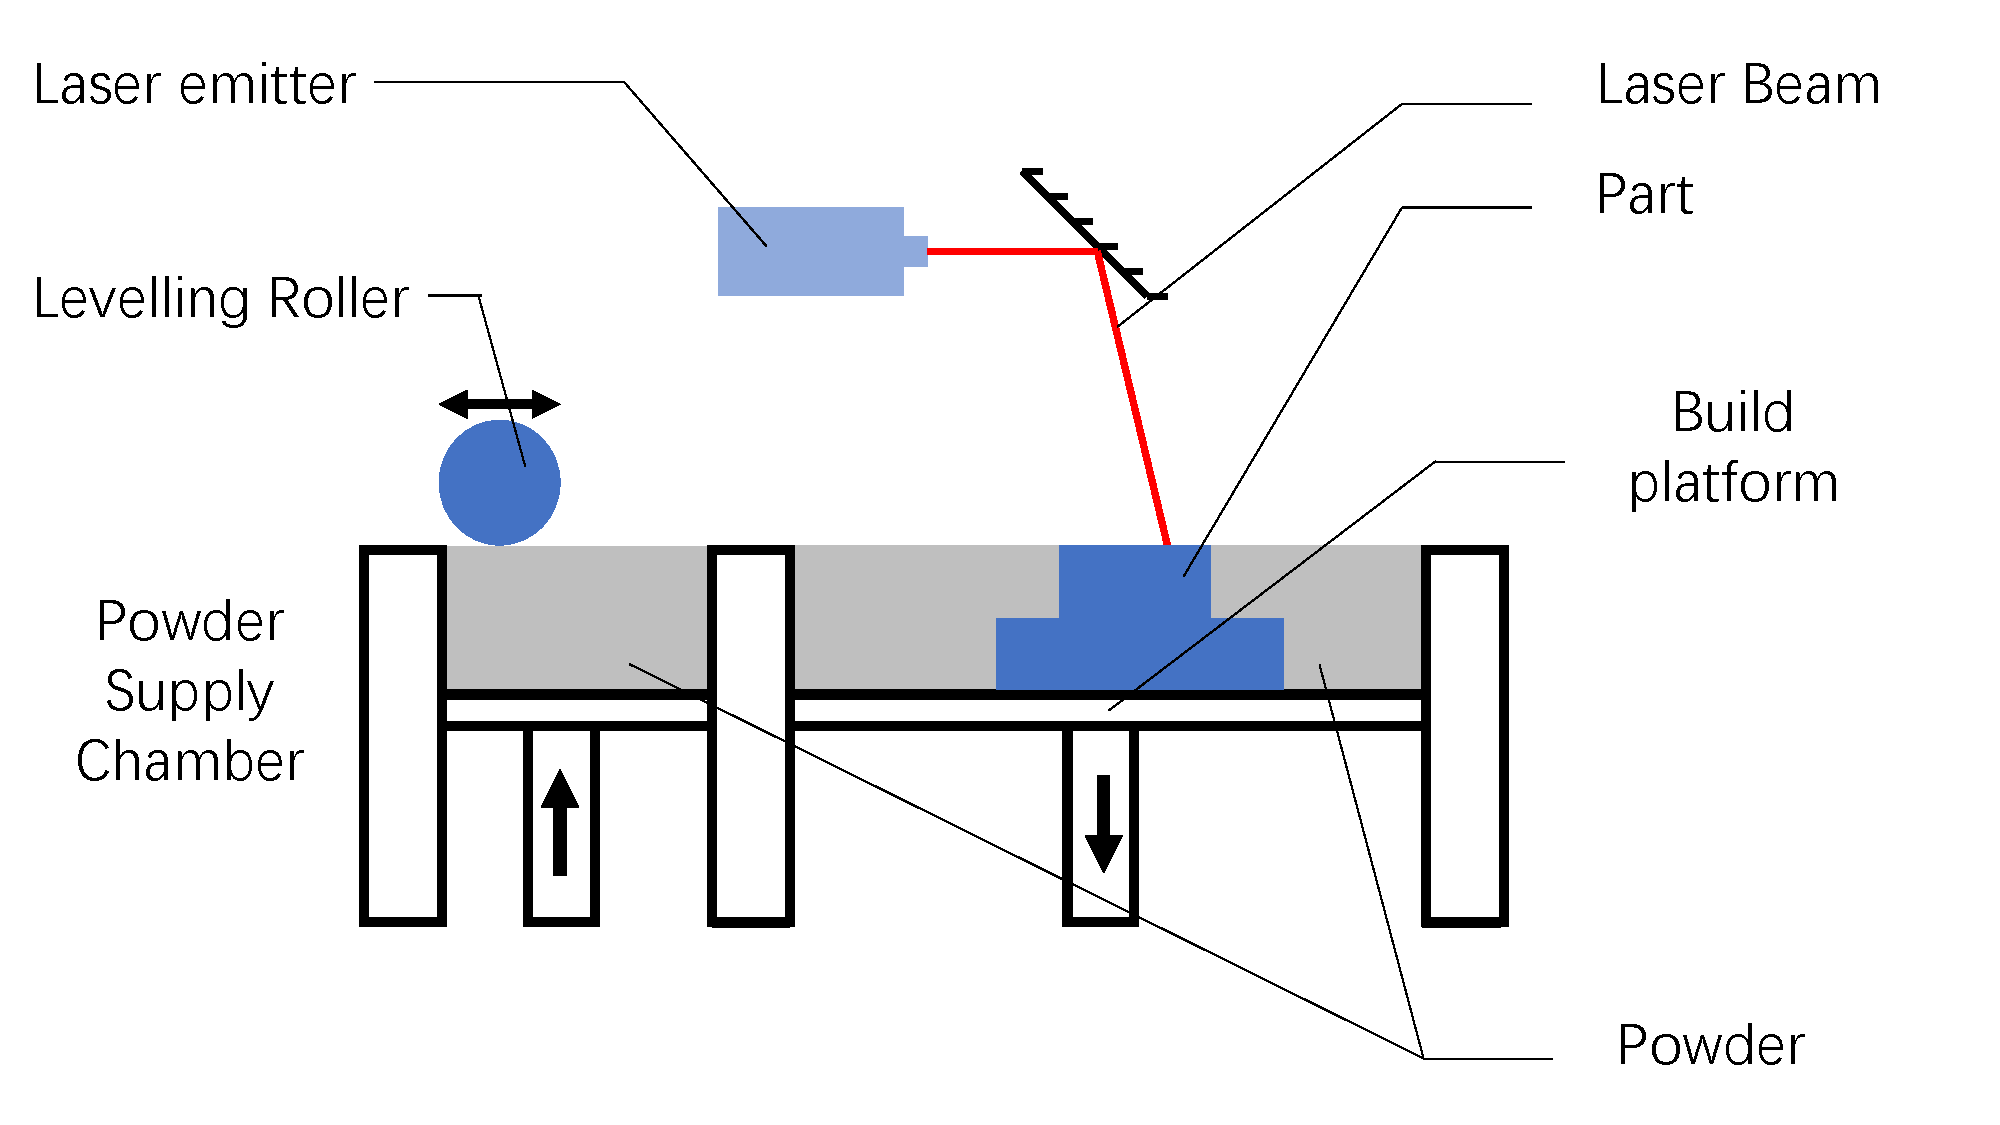
\includegraphics[width=0.9\textwidth]{figures/pbflbm.pdf}
    \caption{Laser-based Powder Bed Fusion of Metals}
    \label{fig: pbflbm}
\end{figure}


Oliverira et al. \cite{Oliveira.2020} have highlighted that two key operational parameters 
exist within the context of \gls{pbflbm}: the source power and the 
scanning velocity. These two parameters exert an influence on the energy 
density imparted to the metal powder, consequently affecting the resulting 
porosity of the fabricated product. Meanwhile, porosity stands as a 
critical parameter impacting the performance of the final product. 
The researchers \cite{Oliveira.2020} have categorized the porosity of the 
finished product into four distinct classes:

\begin{itemize}
    \item Keyhole Porosity: Excessive energy density inhibits the conduction 
    of the melt pool on the powder bed, leading the melt pool to transition 
    into a keyhole mode.
    \item Lack-of-Fusion Porosity: Insufficient energy density results in 
    incomplete fusion of the metal powder, leading to the formation of 
    porosity.
    \item "Balling" (Plateau-Rayleigh instability): Simultaneously employing 
    high source power and excessively elevated scanning velocity induces 
    instability during the processing operation.
    \item Fully-dense porosity: The ideal energy density enables the 
    component to attain a fully dense part.
\end{itemize}


Matthews et al. \cite{Matthews.2017} pointed out that in order to determine 
the evolution of the material's microstructure, information such as 
cooling rate, thermal histories, and material properties are imperative. 
This underscores the necessity of monitoring the \gls{pbflbm} process.

\section{Process monitoring}%
Li et al. \cite{Li.2019} emphasized that in-situ temperature measurement is 
of significant importance for characterizing the mechanical properties of 
materials. In-situ temperature measurement can be categorized into 
in-contact technique and non-contact technique. Given that the temperature 
of the material is high (exceeding 1000$^\circ$C), the region being heated by laser 
is small, and the cooling rate as well as the heating rate is high, 
contact-based measurements would encounter substantial interference, 
thereby rendering the obtained temperature information unreliable. 
Consequently, it becomes essential to employ non-contact-based 
temperature measurement methods.


In the realm of non-contact temperature measurement, 
various measurement systems encompassing ultrasonic, acoustic, and optical 
techniques are present. Within the context of \gls{pbflbm}, 
optical sensors are extensively utilized\cite{Krauss.2012}.


Mani et al. \cite{Mani.2017} pointed out that thermographic imaging in the 
context of Additive Manufacturing (\gls{am}) can be classified into two 
categories based on the optical pathway of the imaging system. 
One category involves aligning the field of view of the sensor with 
the laser beam\cite{Craeghs.2010b,Craeghs.2012,Chivel.2010,Bammer.2010,Berumen.2010,Lott.2011,Yadroitsev.2014}. 
This alignment enables the field of view to track the laser beam, 
allowing for the observation of the melt pool and its scan trajectory.
In addition, an alternative approach involves placing the sensor 
independently of the laser beam. This configuration enables the 
field of view relative static to the material\cite{Craeghs.2012,Dinwiddie.2014,Price.2012,Price.2013,Rodriguez.2012,Wegner.2011}.


Ueda et al. designed the first infrared pyrometer (single-wavelength temperature 
measurement) to measure the temperature. This approach relies on the principles outlined in 
Planck's law, which delineates the interplay between temperature, 
wavelength, and radiative intensity, enabling the measurement of the 
temperature of the object\cite{Ueda.1986}. Subsequently, Dinwiddie et al. 
applied this method for temperature measurement in electron beam melting\cite{Dinwiddie.2014}. 
Meanwhile, Krauss et al. employed this technique to identify defects 
and discontinuous failure spots arising during the \gls{am} process\cite{Krauss.2012}.


However, due to the intricate nature of temperature in real cases, the 
single-wavelength temperature measurement approach may lead to 
misrepresentations of temperature measurement. The models employed in 
single-wavelength temperature measurement methods lack appropriate 
parameters, rendering them susceptible to interference and unable to 
accurately depict the phenomenon of changing emissivity with 
increasing wavelength\cite{Raplee.2017}.





%
%
\section{Multispectral imaging}%

%
%
\section{Emissivity model}%

%
%
\section{Temperature estimation algorithm}


\section{Motivation of this thesis}%
% !TeX spellcheck = en_US
\chapter{Theory and methodology}%
As mentioned in previous sections, forming a virtual experiment platform 
is necessary for investigating the temperature estimation algorithm. So, a virtual 
experiment platform is developed based on Planks'law, then, a virtual multi-spectral 
pyrometer is applied to obtain the digital value (also called image). 


\section{Physical value of radiation}%
Radiation is emitted from any object with a temperature above $0 \, \text{K}$. In equation \ref{eq: radiation_pv}
can be found, that the radiation depends on the black body radiation $B(\lambda, T)$ 
and emissivity $\varepsilon(\lambda, T)$. Both value are temperature $T$ and wavelength $\lambda$ 
dependent.

\begin{equation}
    \label{eq: radiation_pv}
    L(\lambda, T) = B(\lambda, T) \cdot \varepsilon (\lambda, T)
\end{equation}


By Plank's Law, black body radiation can be described in equation \ref{eq: planks_law}, 
with absolute temperature $T$, wavelength $\lambda$, speed of light $c$, Plank 
constant $h$ and Boltzmann constant $k_B$. Black body radiation is irrelevant 
to the material itself, all materials at the same temperature have the same spectral 
black body radiation.

\begin{equation}
    \label{eq: planks_law}
    B(\lambda, T) = \frac{{2hc^2}}{{\lambda^5}} \cdot {\left[{\exp\left(\frac{{hc}}{{\lambda k_B T}}\right) - 1}\right]}^{-1}
\end{equation}


On the contrary, emissivity varies from material to material. It is the 
ratio of the actual spectral intensity emitted by the object to the spectral 
intensity of the black body radiation. In the study of radiation, two idealized 
material models are generally used to describe the idealized 
properties of radiation, namely black body and grey body. 


Black-body material emits electromagnetic black body radiation, which is irrelevant to 
the wavelength of the radiation and the shape of the material\cite{Kuhn.1987}. Which 
also means the emissivity of a black body is constantly 1. It could be used to validate
the temperature estimation algorithm in following sections.


Unlike black-body materials, grey-body materials have an emissivity between 0 and 1.
Not all of the thermal radiation could be emitted to the outside of the material. 
Different from normal materials, the emissivity of a grey-body material is irrelevant
to the wavelength of radiation.

\begin{figure}[htbp]
    \centering
    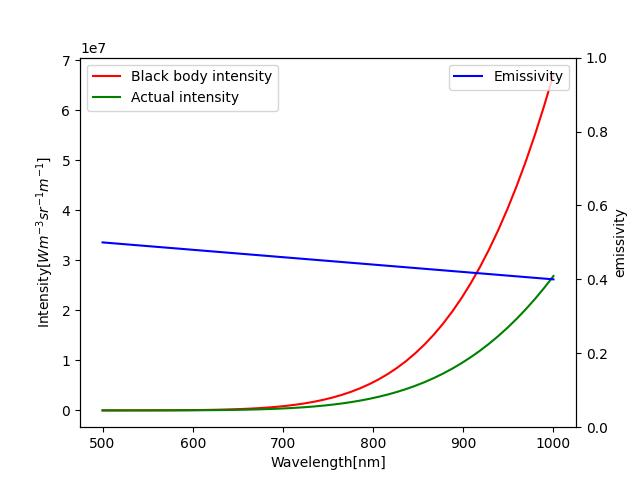
\includegraphics[width = 0.8\textwidth]{figures/real_radiation.jpg}
    \caption{Black body radiation, emissivity and real radiation of an example normal
    material at $1000K$}
    \label{fig: black_body_radiation}
\end{figure}


In Fig.\ref{fig: black_body_radiation} can be found, that the real spectral 
intensity of a normal material is lower than the black body spectral intensity.
And the emissivity of the material varies with the increase of the radiation 
wavelength.


It can be seen that the construction of a reliable emissivity model is crucial to 
the accuracy of the virtual experimental platform. It is the key component used to 
generate the experimental data.




\section{Virtual experiment platform}%
After obtaining the physical spectral intensity of the material, a virtual experiment platform
is used to transform the physical value into digital value, which simulate the 
behavior of a real spectral pyrometer. As described in Fig.\ref{fig: virtual_platform}, a 
camera with a lens system focused on the surface of the powder bed is resonsible 
for obtaining spectral radiation of the heated metal powder. It can be seen from 
Fig.\ref{fig: sensor_pixel}, each pixel of the sensor 
contains 8 filters and thus be able to obtain 8 intensity digital values in different 
channels. Thus, a virtual experiment platform with the same structure as the real 
experiment platform is built.

\begin{figure}[htbp]
    \centering
    \begin{subfigure}{0.6\textwidth}
        \centering
        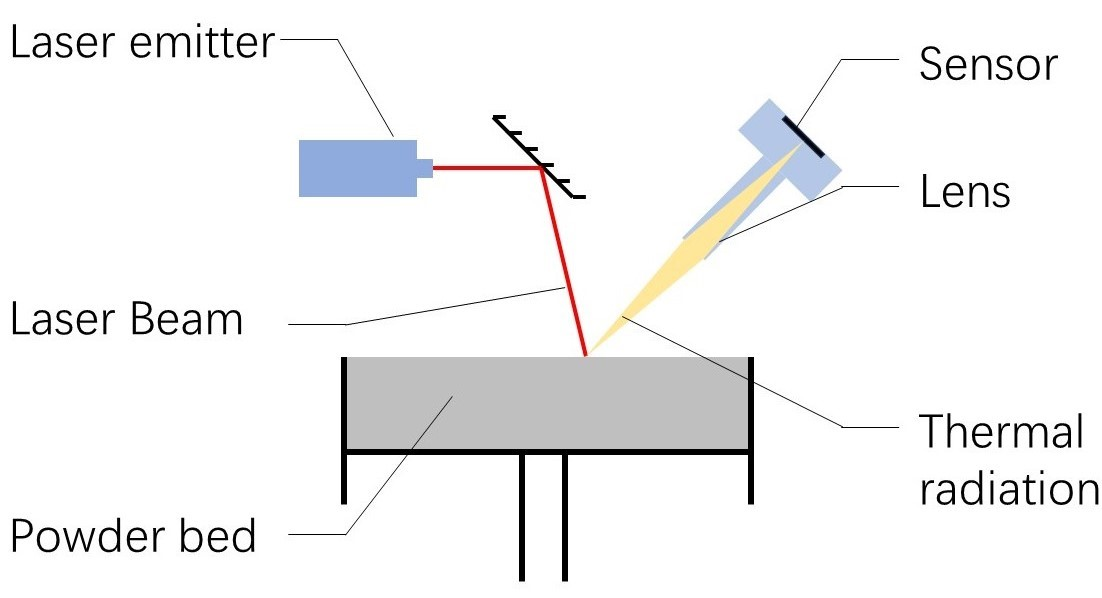
\includegraphics[height=4.8cm]{figures/virtual_platform.jpg}
        \caption{Virtual experiment platform}
        \label{fig: virtual_platform}
    \end{subfigure}
    \hfill
    \begin{subfigure}{0.37\textwidth}
        \centering
        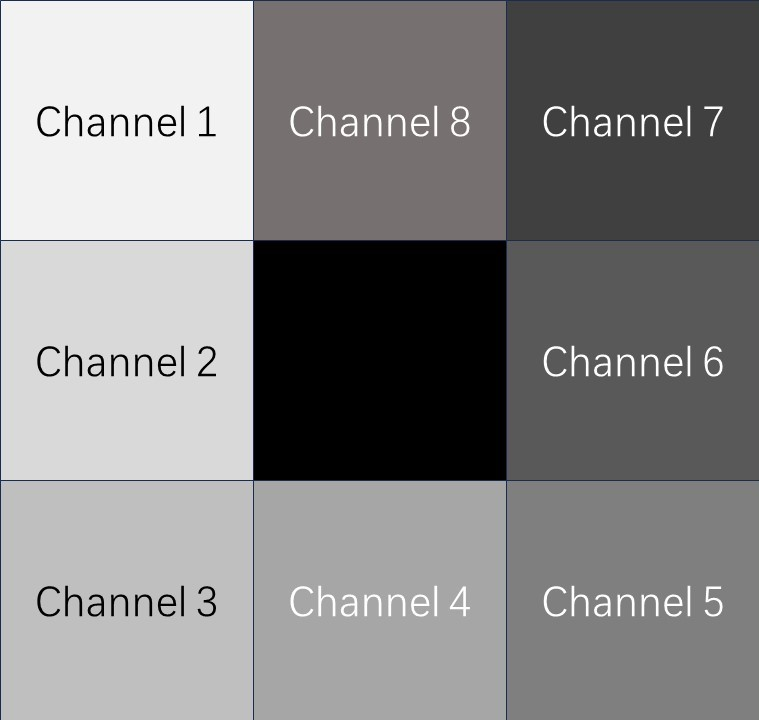
\includegraphics[height=5cm]{figures/sensor_pixel.jpg}
        \caption{Layout of a sensor pixel}
        \label{fig: sensor_pixel}
    \end{subfigure}
    \caption{Structure of the virtual experiment platform and Layout of a sensor pixel}
    \label{fig: virtual_pixel}
\end{figure}


\section{Camera model}
It can be found in Fig.\ref{fig: virtual_pixel}, The thermal radiation is emitted from the surface of powder bed, and passes through 
the lens system of the camera, finally, it reaches the sensor and be converted into 
digital values. The simplified process can be seen in Fig.\ref{fig: view_factor}. $dA_m$ is the 
area of the focused surface and $dA_{pixel}$ the area of the pixel in camera system, $n_m$ is the 
normal vector of the surface.

\begin{figure}[htbp]
    \centering
    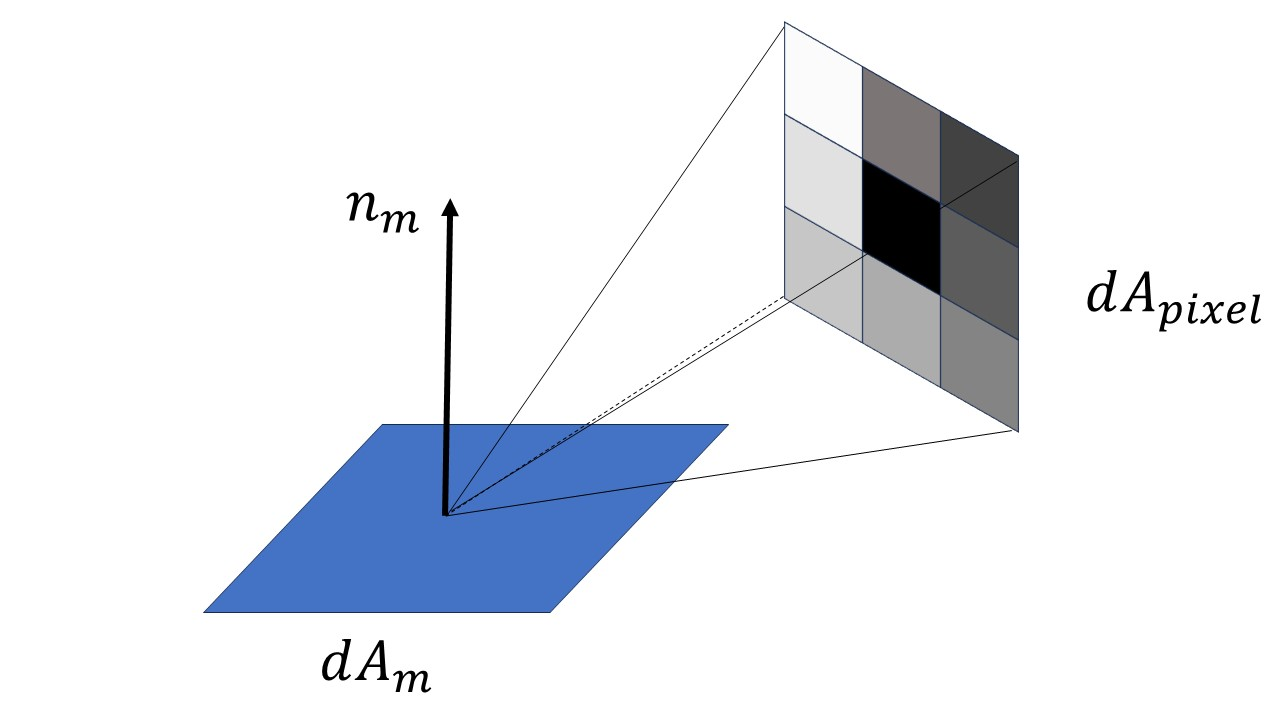
\includegraphics[width=0.6\textwidth]{figures/view_factor.jpg}
    \caption{Radiative exchange between camera system and powder bed}
    \label{fig: view_factor}
\end{figure}


\begin{comment}
Thus, the radiation intensity received by the camera system can be expressed in Eq.\ref{eq: physical_value_received}.
Where $dL_{sensor}$ means the spectral intensity reached on each channel, $dL_{material}$
is the spectral intensity emitted from the surface area, $\phi_{dA_m - dA_{pixel}}$ is the 
view factor between the focused surface area and camera system.

\begin{equation}
    \label{eq: physical_value_received}
    dL_{sensor} =  dL_{material} \cdot \phi_{dA_m - dA_{pixel}}
\end{equation}


The view factor describes the ratio between the emitted intensity of the surface area 
and the received intenisty by the pixel in camera. It only relates to the shape of 
the two surfaces and the geometric position between them\cite{Rohsenow.1998}. Since 
in real experiments, the sensor is fixed in a certain position on the machine while the 
surface of the powder bed does not move relatively to the machine, it can be concluded
that the geometry of the camera system and the focused area does not change. This means that 
the view factor does not change as the process proceeds.


So, in order to simplify the physical model of the virtual experiment platform and 
thus avoid unnecessary complexity, one assumption was made that the view factor between 
surface area of the powder bed and the camera system is constantly set to 1.
\end{comment}


\subsection{Frequency response}
After obtaining the virtual experiment platform and knowing the external setup of the 
sensor, the internal effects of the camera system should also be taken into account 
in the complete virtual experiment platform.


In order to simulate real camera system, the frequency response of sensor and lens 
should be considered. In real camera systems, all spectral radiation will 
pass through the lens system of camera. Since the lens system is not an 
idealized system, the effect of the lens system is not negligible. 

\begin{figure}[htbp]
    \centering
    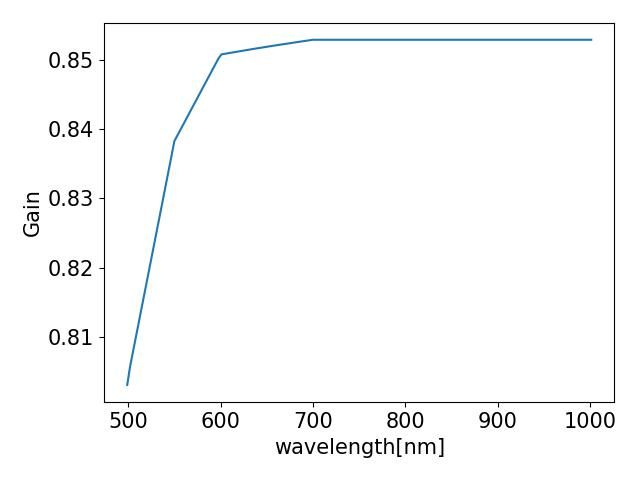
\includegraphics[width=0.6\textwidth]{figures/tr_frequency_response.jpg}
    \caption{Frequency response of the lens system}
    \label{fig: frequency_response_lens}
\end{figure}


It can be found in Fig.\ref{fig: frequency_response_lens} that system gain 
of lens system is not constant. In the wavelength range of 500 to 700 nanometers, 
the lens is more sensitive to the radiation with long wavelength. With the 
increasing wavelength, the system gain of the lens system keep constant at 0.853.


In addition to the fact that the lens system respond differently to radiation
with different wavelengths, the sensor of the camera also have wavelength-dependent quantum 
efficiency. As mentioned in previous section, the acquisition of the spectral 
intensity by the sensor for different channels is based on the filter 
before the pixels. 


Fig.\ref{fig: quantum_efficiency} shows the quantum efficiency 
of the camera sensor in different channels. Unlike an ideal sensor that 
receives only single wavelength radiation, the intensity information received 
by a real sensor is a combination of a spectral radiation and 8 filters with 
different frequency responses. Thus, the camera system is able to obtain the 
spectral radiation intensity in 8 channels simutaneously. 


\begin{figure}[htbp]
    \centering
    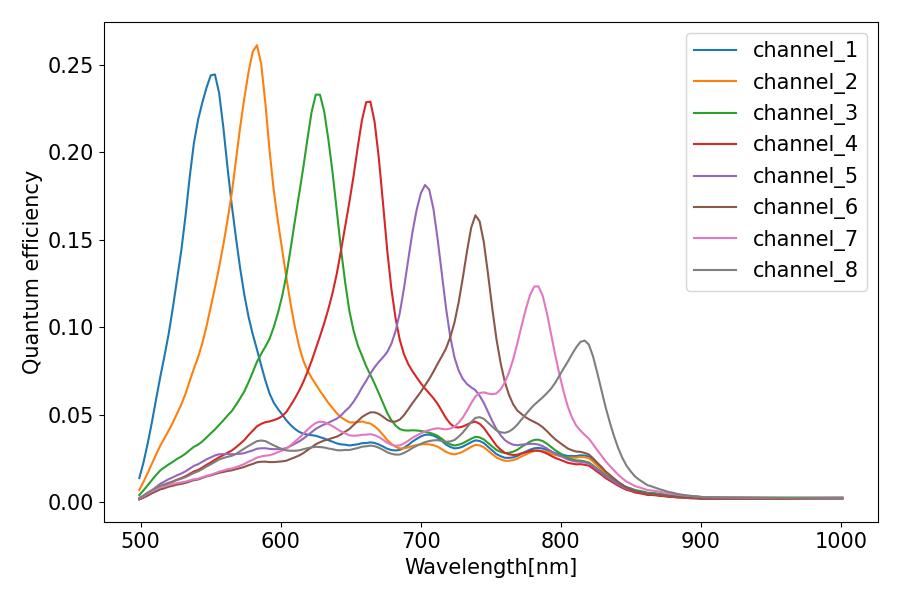
\includegraphics[width = 0.8\textwidth]{figures/quantum_efficiency.jpg}
    \caption{Quantum efficiency of camera system in each channel}
    \label{fig: quantum_efficiency}
\end{figure}


To make the virtual experiment platform more comparable to real experiments, 
it can be concluded that it is necessary to build a camera model that 
incorporates the effects of sensor quantum efficiency and lens transparency.
Then, the physical value of the spectral radiation intensity could be 
calculated accurately by the digital value of spectral radiation intensity obtained from the virtual experiment 
platform.


\subsection{Integration method}
As a result, the process of converting the physical values of radiation intensity 
into digital values needs to be accurately reproduced. Since the total efficiency 
of the camera (${\eta}_{camera}$) was delivered by quantum efficiency (${\eta}_{quantum}$)
of the sensor and transparency of the lens system{$\tau_{lens}$}, the mathematical
relationship could be described in Eq.\ref{eq: cam_efficiency}.


\begin{equation}
    \label{eq: cam_efficiency}
    {\eta}_{camera} = {\eta}_{quantum} \cdot \tau_{lens}
\end{equation}


Fig.\ref{fig: received} shows the relationship between the incoming spectral 
radiation intensity and actual captured spectral radiation intensity 
by the camera system. It can be found that the wavelength of the spectral 
radiation intensity actually received by the sensor deviates from the wavelength of the 
spectral radiation intensity it supposed to receive.


\begin{figure}[htbp]
    \centering
    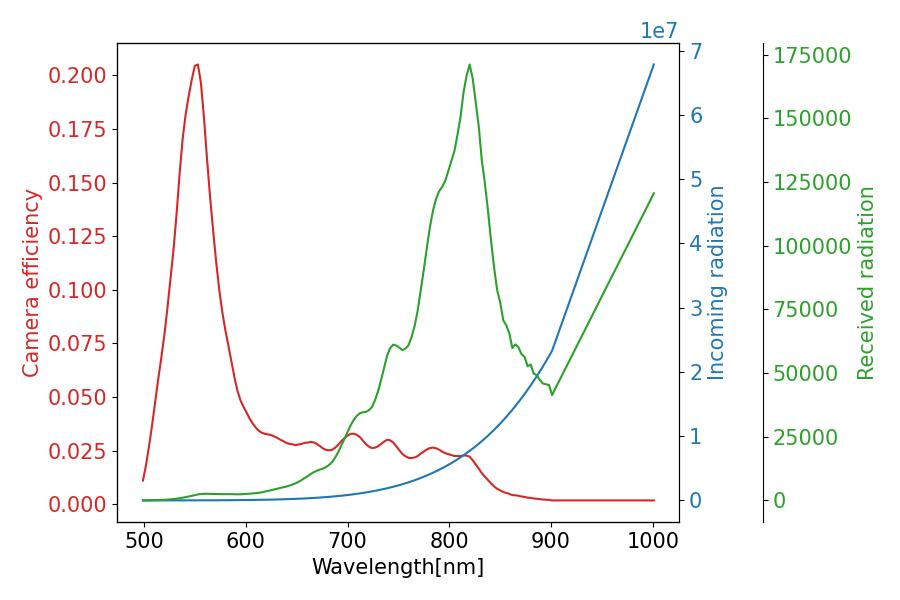
\includegraphics[width = 0.8\textwidth]{figures/received_radiation.jpg}
    \caption{Actual received spectral radiation intensity by channel 1 at 1000K}
    \label{fig: received}
\end{figure}


Obtaining the physical value of spectral radiation intensity, the sensor is responsible 
for transforming the physical value into digital value for upcoming proceedings.
The camera system used in real experiment platform uses \gls{ccd} or \gls{cmos}
as their sensors. Both sensors transform the photon flux $\phi (\lambda)$ 
incident on the semiconfuctor into photocurrent $I_{ph}$\cite{Fossum.2014}. 

\begin{equation}
    \label{eq: principle_cmos}
    I_{ph} = q \int_{\lambda}^{} \phi(\lambda) \cdot \eta_{camera}(\lambda) d\lambda
\end{equation}

With a certain temperature $T$: 

\begin{equation}
    \label{eq: quantum_flux_intensity}
    \phi(\lambda) = L(\lambda, T)
\end{equation}

Eq.\ref{eq: principle_cmos} is the mathetical description of the 
transformation. Where $\phi(\lambda)$ denotes photon flux on the sensor, 
which is equal to the spectral radiation intensity on the sensor $L(\lambda, T)$ as 
described in Eq.\ref{eq: quantum_flux_intensity}, and $\eta_{camera}(\lambda)$
denotes the total efficiency of the camera in Eq.\ref{eq: cam_efficiency}. $q$ is the sensitivity parameter 
of the sensor.


\subsection{Implementation}
Similar to the method used to obtain the digital value of spectral radiation intensity 
in the real experiment, the virtual experiment platform calculates the 
intensity digital value in 8 channels using the virtual camera by entering 
the material properties of the point being measured.


\begin{figure}[htbp]
    \centering
    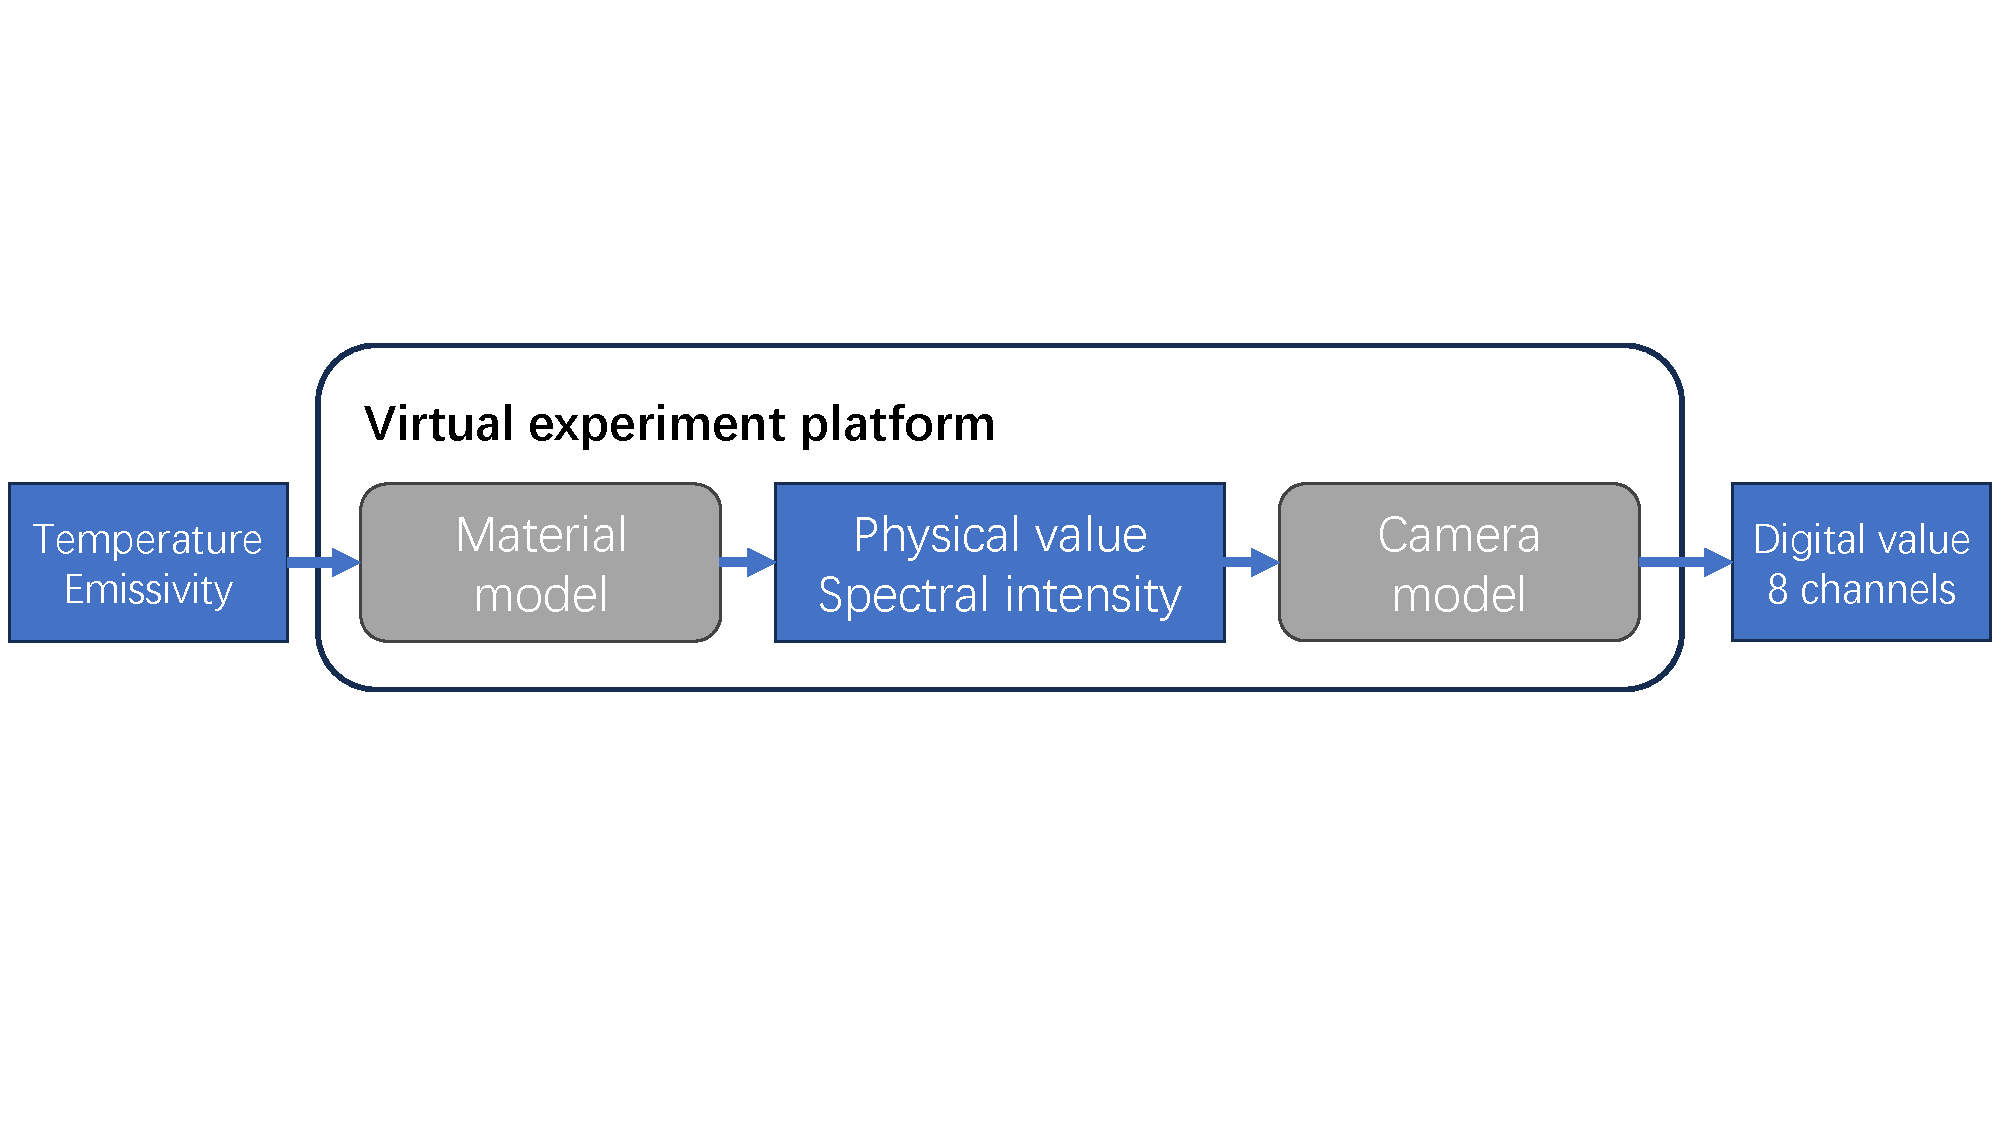
\includegraphics[width=0.95\textwidth]{figures/camera_model.pdf}
    \caption{Procedure of using virtual experiment platform to generate digital values}
    \label{fig: process_virtual_platform}
\end{figure}

Fig.\ref{fig: process_virtual_platform} shows the working procedure of the 
virtual experiment platform. 
To enable the virtual experimental platform to run on various devices, 
the entire platform has been implemented using Python as the 
programming language and packaged into a .py file. Furthermore, all 
functions have been vectorized to facilitate the generation of image 
outputs resembling those captured by a physical camera. Additionally, 
the parallel computing package in Python has been utilized to minimize 
computation time.


\section{Temperature estimation algorithm}
After obtaining the experimental data calculated by the virtual experiment platform, 
a temperature estimation algorithm should be developed to calculate the temperature 
of the measured point based on the experimental data.


Similar to the set up in real experiments, the parameters of the camera model can be 
considered as known in the virtual experimental platform mentioned in this article. 
This will on the one hand improve the accuracy of the temperature estimation algorithm
and on the other hand avoid some unnecessary complexity.


Thus, in this temperature estimation algorithm, the known variable is the digital value of 
spectral intensity captured by camera model in virtual experiment platform, the characteristic 
of the camera system. The variables to be estimated are the temperature of the measured point and 
its emissivity.


\begin{figure}[htbp]
    \centering
    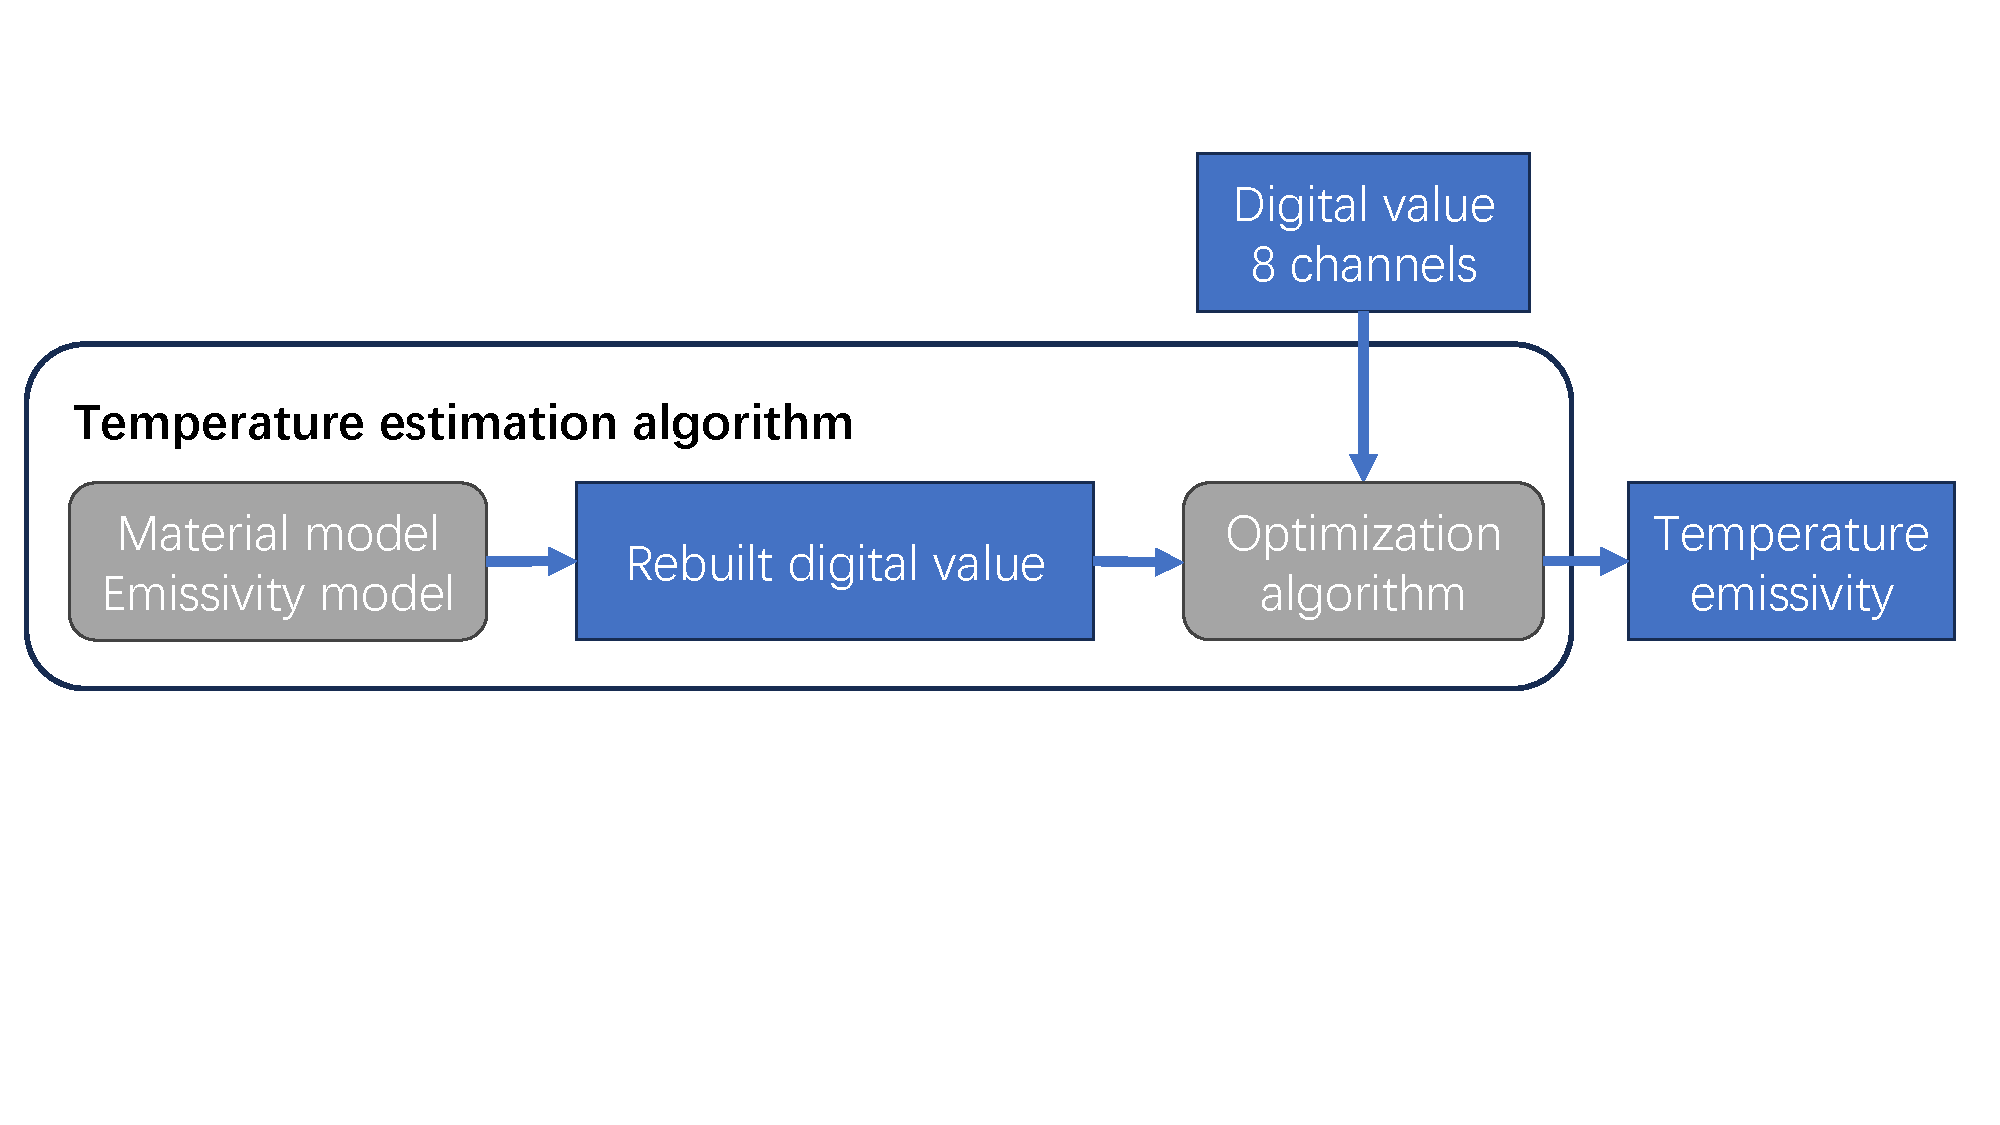
\includegraphics[width=0.95\textwidth]{figures/temperature_esti_algorithm.pdf}
    \caption{Procedure of temperature estimation algorithm}
    \label{fig: temperature_estimation_algorithm}
\end{figure}


\subsection{Temperature estimation with integration method}
Fig.\ref{fig: temperature_estimation_algorithm} shows the proceeding procedure of the 
temperature estimation algorithm. The digital value of the spectral radiation intensity
$(I_{rec}(i))$ 
in the $i_{th}$ channel should be reconstructed in Eq.\ref{eq: reconstruct_integration}:

\begin{equation}
    \label{eq: reconstruct_integration}
    I_{rec}(i) = q \int B(\lambda, T) \cdot \varepsilon(\lambda, k, T) \cdot \eta_{camera}(i) d\lambda
\end{equation}

With $I_{DV}(i)$ the reconstructed digital value in $i_{th}$ channel, $B(\lambda, T)$ the black body radiation, 
$\varepsilon(\lambda, k, T)$ the emissivity model in temperature estimation algorithm, 
$\eta_{camera}(i)$ the total camera efficiency of $i_{th}$ channel. It can be found that 
the emissivity model have an additional parameter $k$, this parameter is used for fitting 
the emissivity behavior of the measured material. More details can be found in the following 
section.


Given an initial guess of the status parameters, namely 
temperature($T_0$) and parameters in emissivity model($k_0$). Then, an curve fit 
algorithm is applied to minimize the difference between the reconstructed digital value $(I_{rec})$ 
and the actual digital value $(I_{act})$ in Eq.\ref{eq: reconstruct_optimization}.

\begin{equation}
    \label{eq: reconstruct_optimization}
    \min_{k, T}\sum_{i=1}^{8}  F(I_{rec}(i), I_{act}(i))
\end{equation} 

$F(I_{rec}(i), I_{act}(i))$ is the cost function of the curve fit algorithm. In this 
application, Non-linear least squares method is used to obtain the optimum parameters 
as Eq.\ref{eq: least_square}.

\begin{equation}
    \label{eq: least_square}
    F(I_{rec}(i), I_{act}(i)) = (I_{rec}(i) - I_{act}(i))^2
\end{equation}


After obtaining the estimated temperature ($T_{estimate}$) and the parameter ($k$) 
in the emissivity model, the data will be saved in a .xlsx file for 
potential operations.

\subsection{Temperature estimation with linear method}
To be done


\section{Emissivity model in temperature estimation algorithm}%
As an unknown quantity in the temperature estimation algorithm, the nature of emissivity 
as a function of wavelength also introduces an additional degree of freedom 
into the overall calculation process. In order to provide a more general description of 
the trend of emissivity with wavelength, an additional parameter ($k$) in the 
emissivity model used for temperature estimation has been introduced.


Due to the inherent complexity of this trend, it is often impossible to describe 
the emissivity using a single parameter. Therefore, the parameter ($k$) is normally 
represented as a vector composed of multiple variables. This approach allows for both a 
concise mathematical representation and the incorporation of more 
intricate emissivity models into the temperature estimation algorithm.


%
%
%
%
% Appendix
% --------
\appendix%
\chapter{Appendices}%
\section{Calculation result of temperature estimation algorithm}

\subsection{Linear model}
\begin{figure}[h]
    \centering
    \begin{minipage}{\textwidth}
        \centering
        \begin{subfigure}{0.325\textwidth}
            \centering
            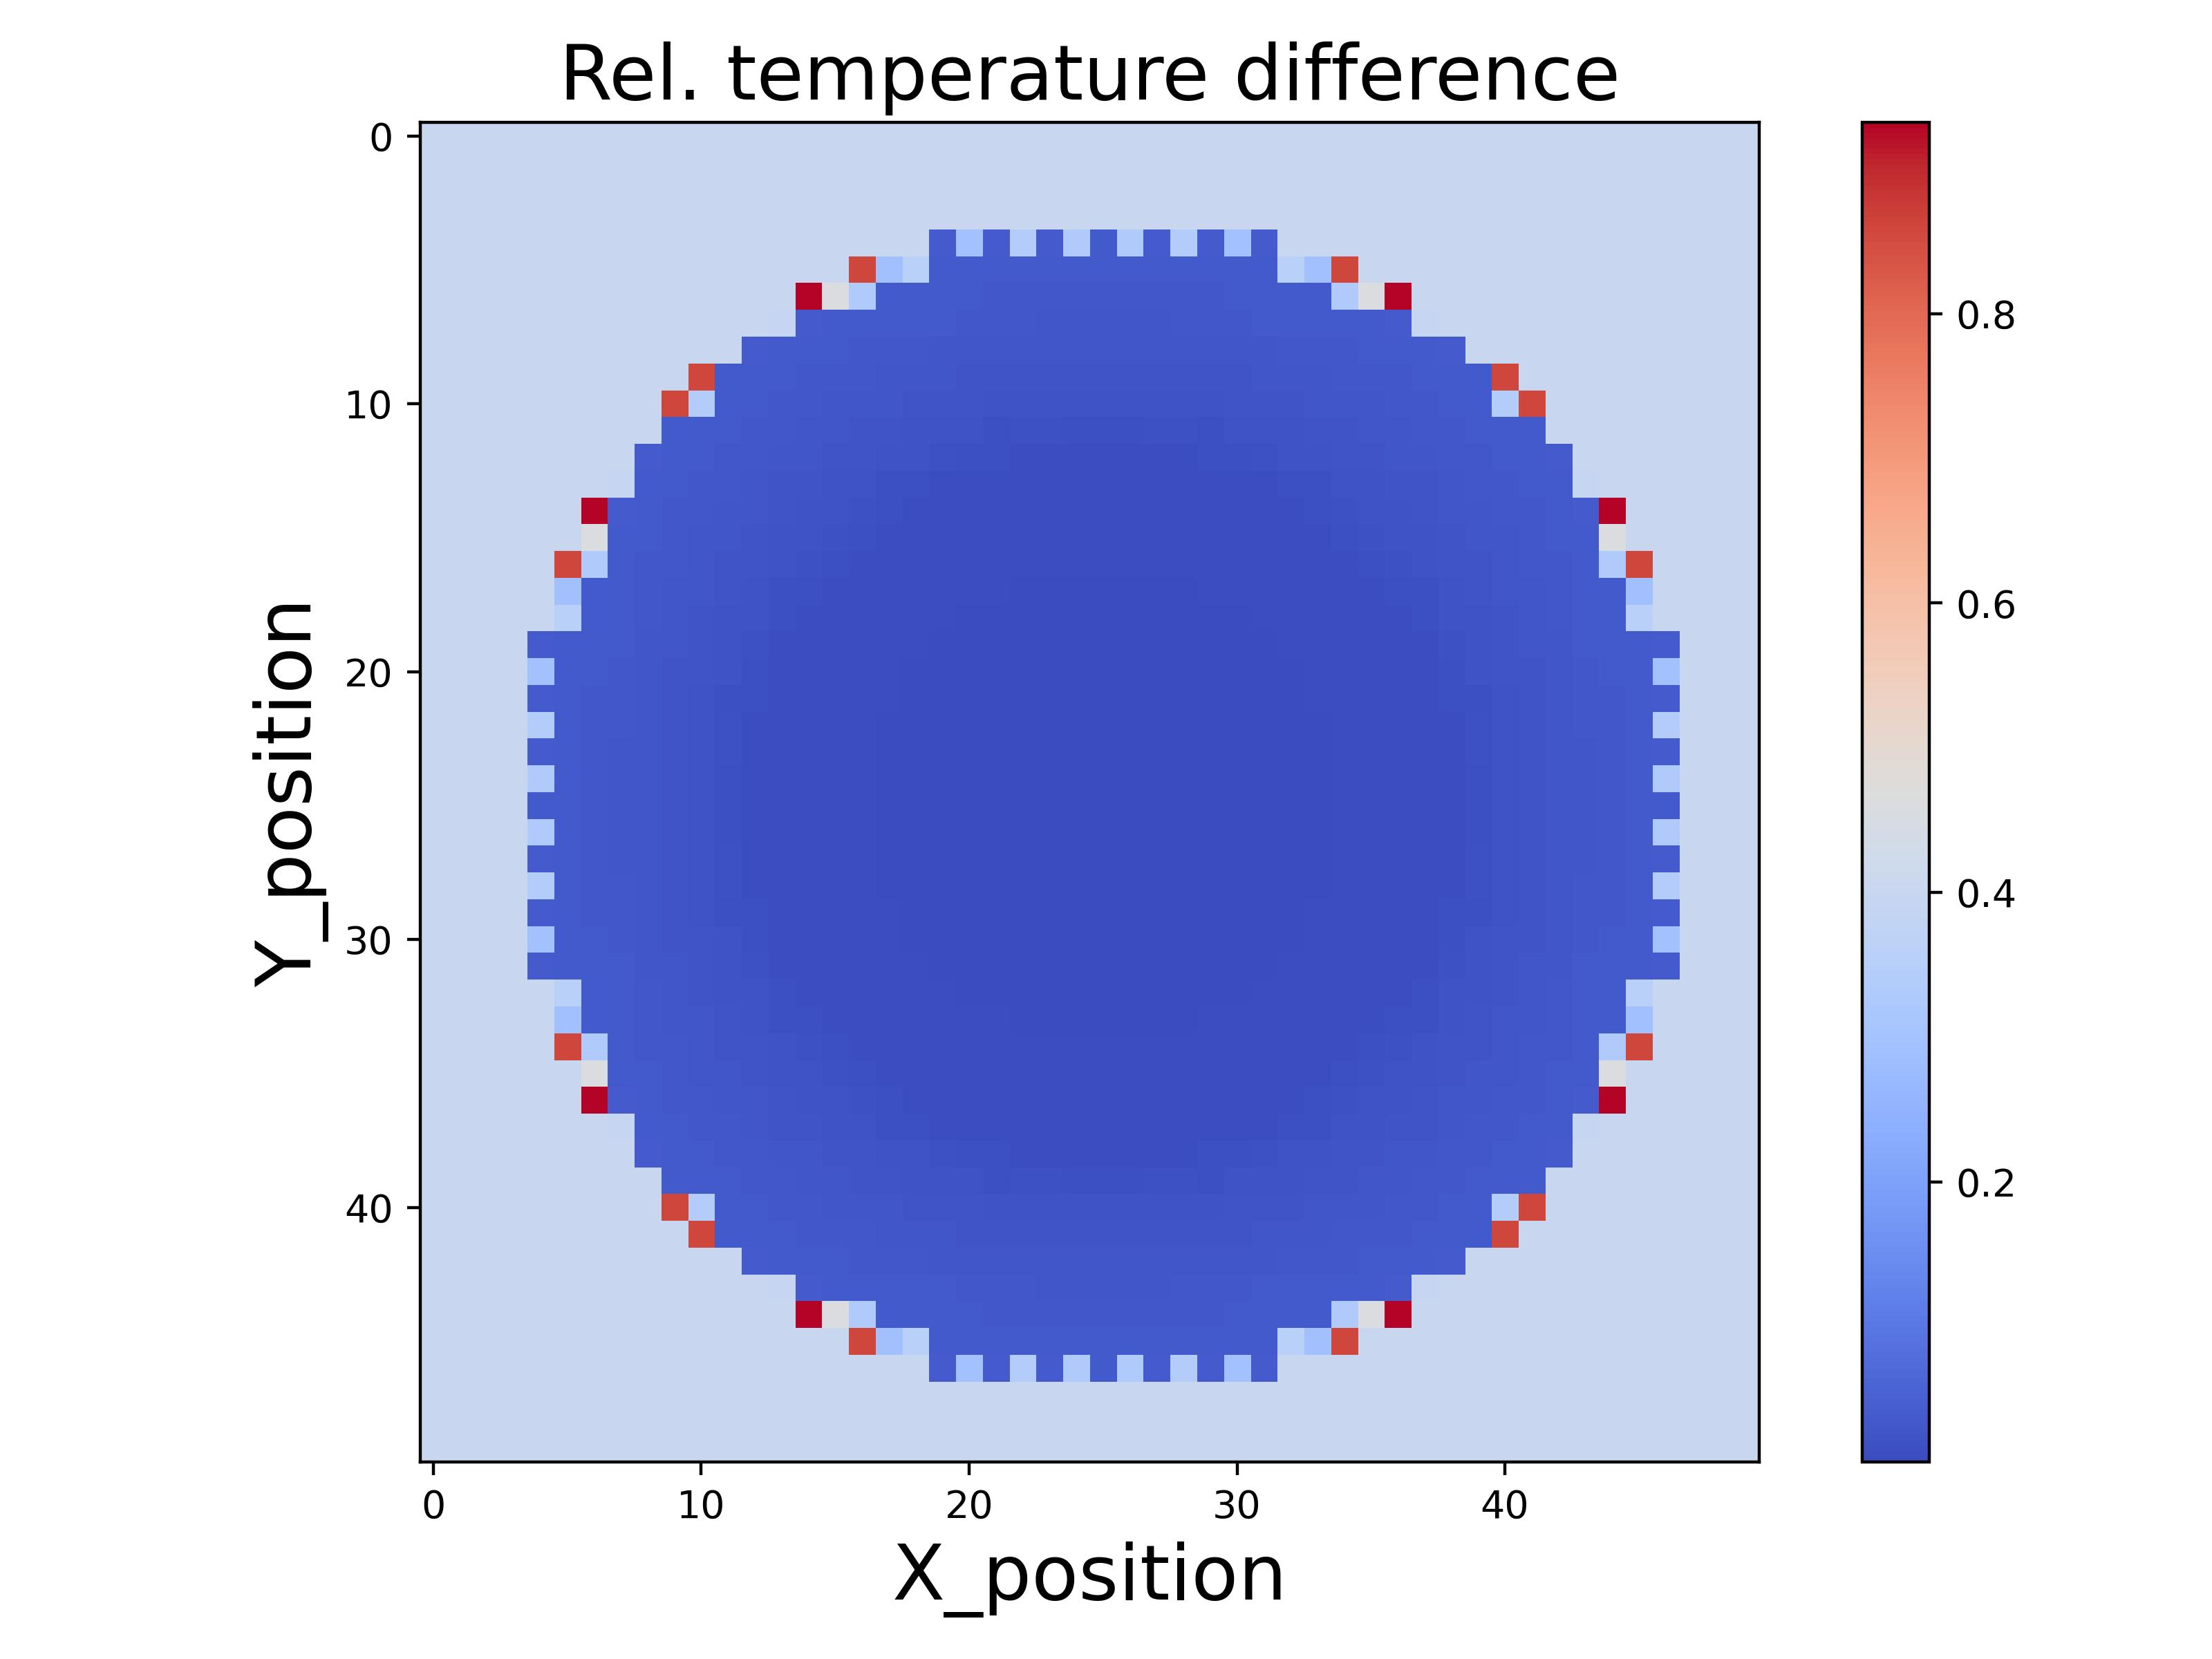
\includegraphics[width=\textwidth]{figures/raw_data/0/linear/T_bias.jpg}
            \subcaption{Black body material}
        \end{subfigure}
        \begin{subfigure}{0.325\textwidth}
            \centering
            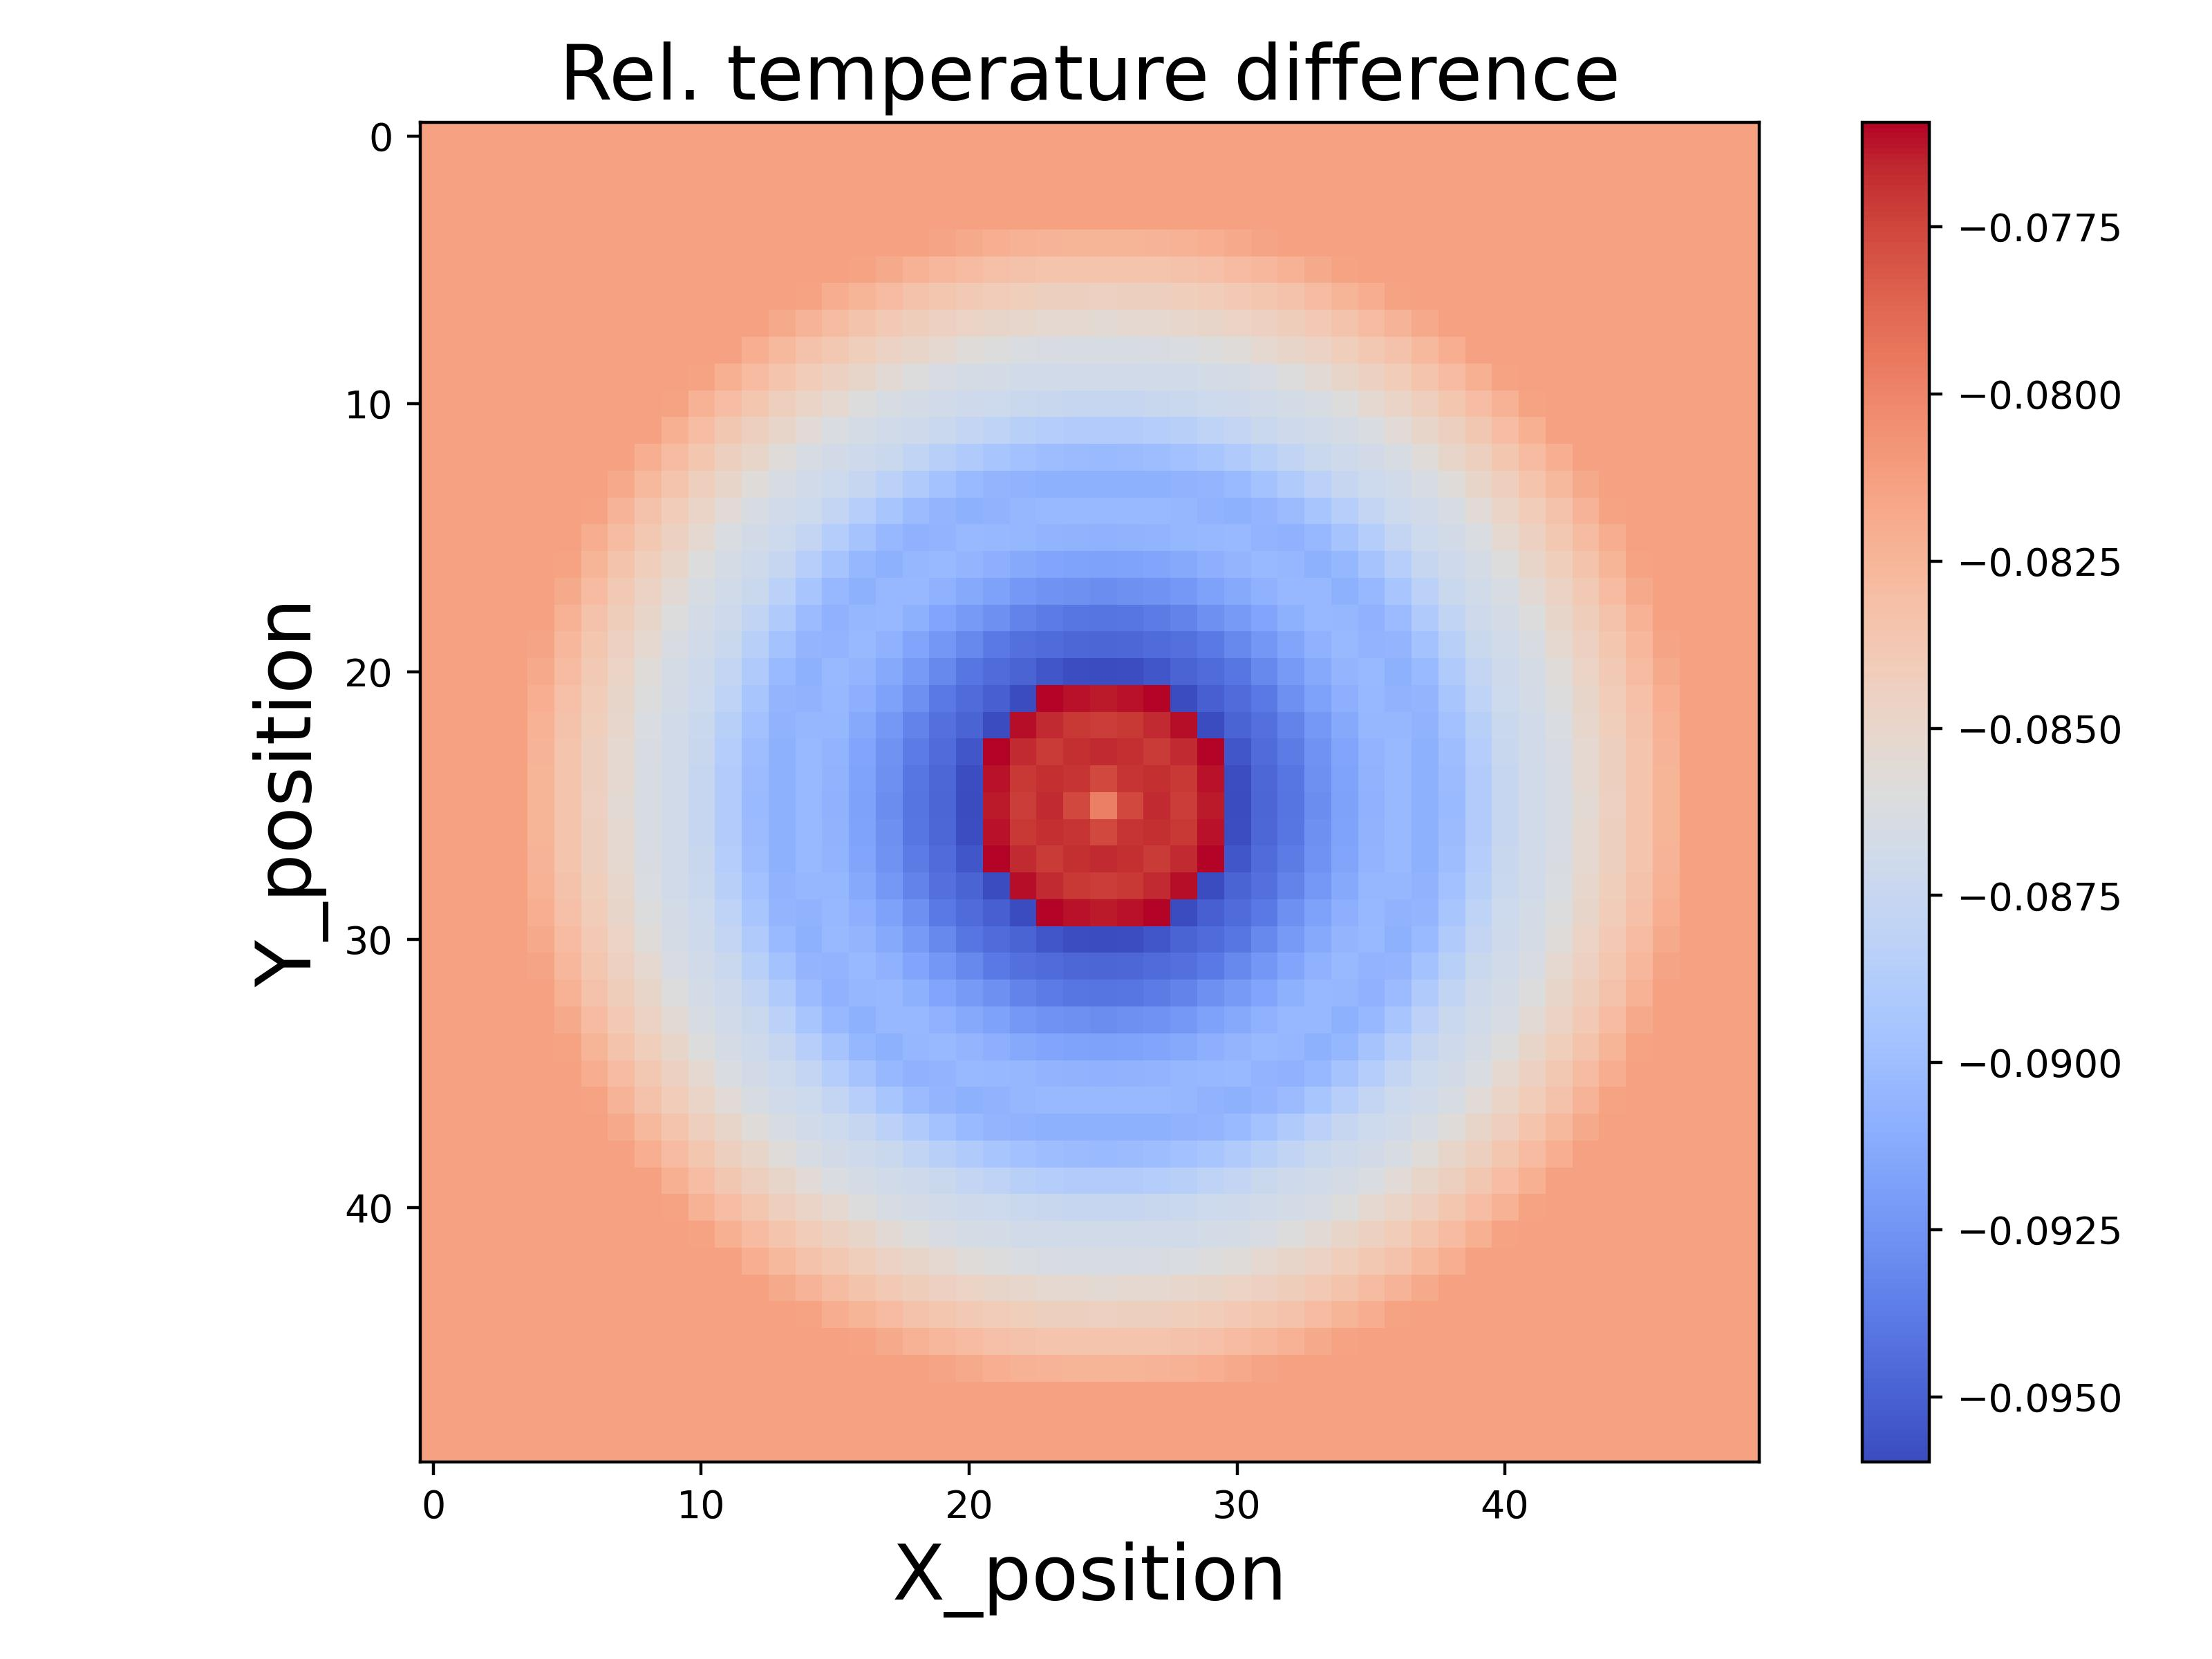
\includegraphics[width=\textwidth]{figures/raw_data/5/linear/T_bias.jpg}
            \subcaption{Real iron data}
        \end{subfigure}
        \begin{subfigure}{0.325\textwidth}
            \centering
            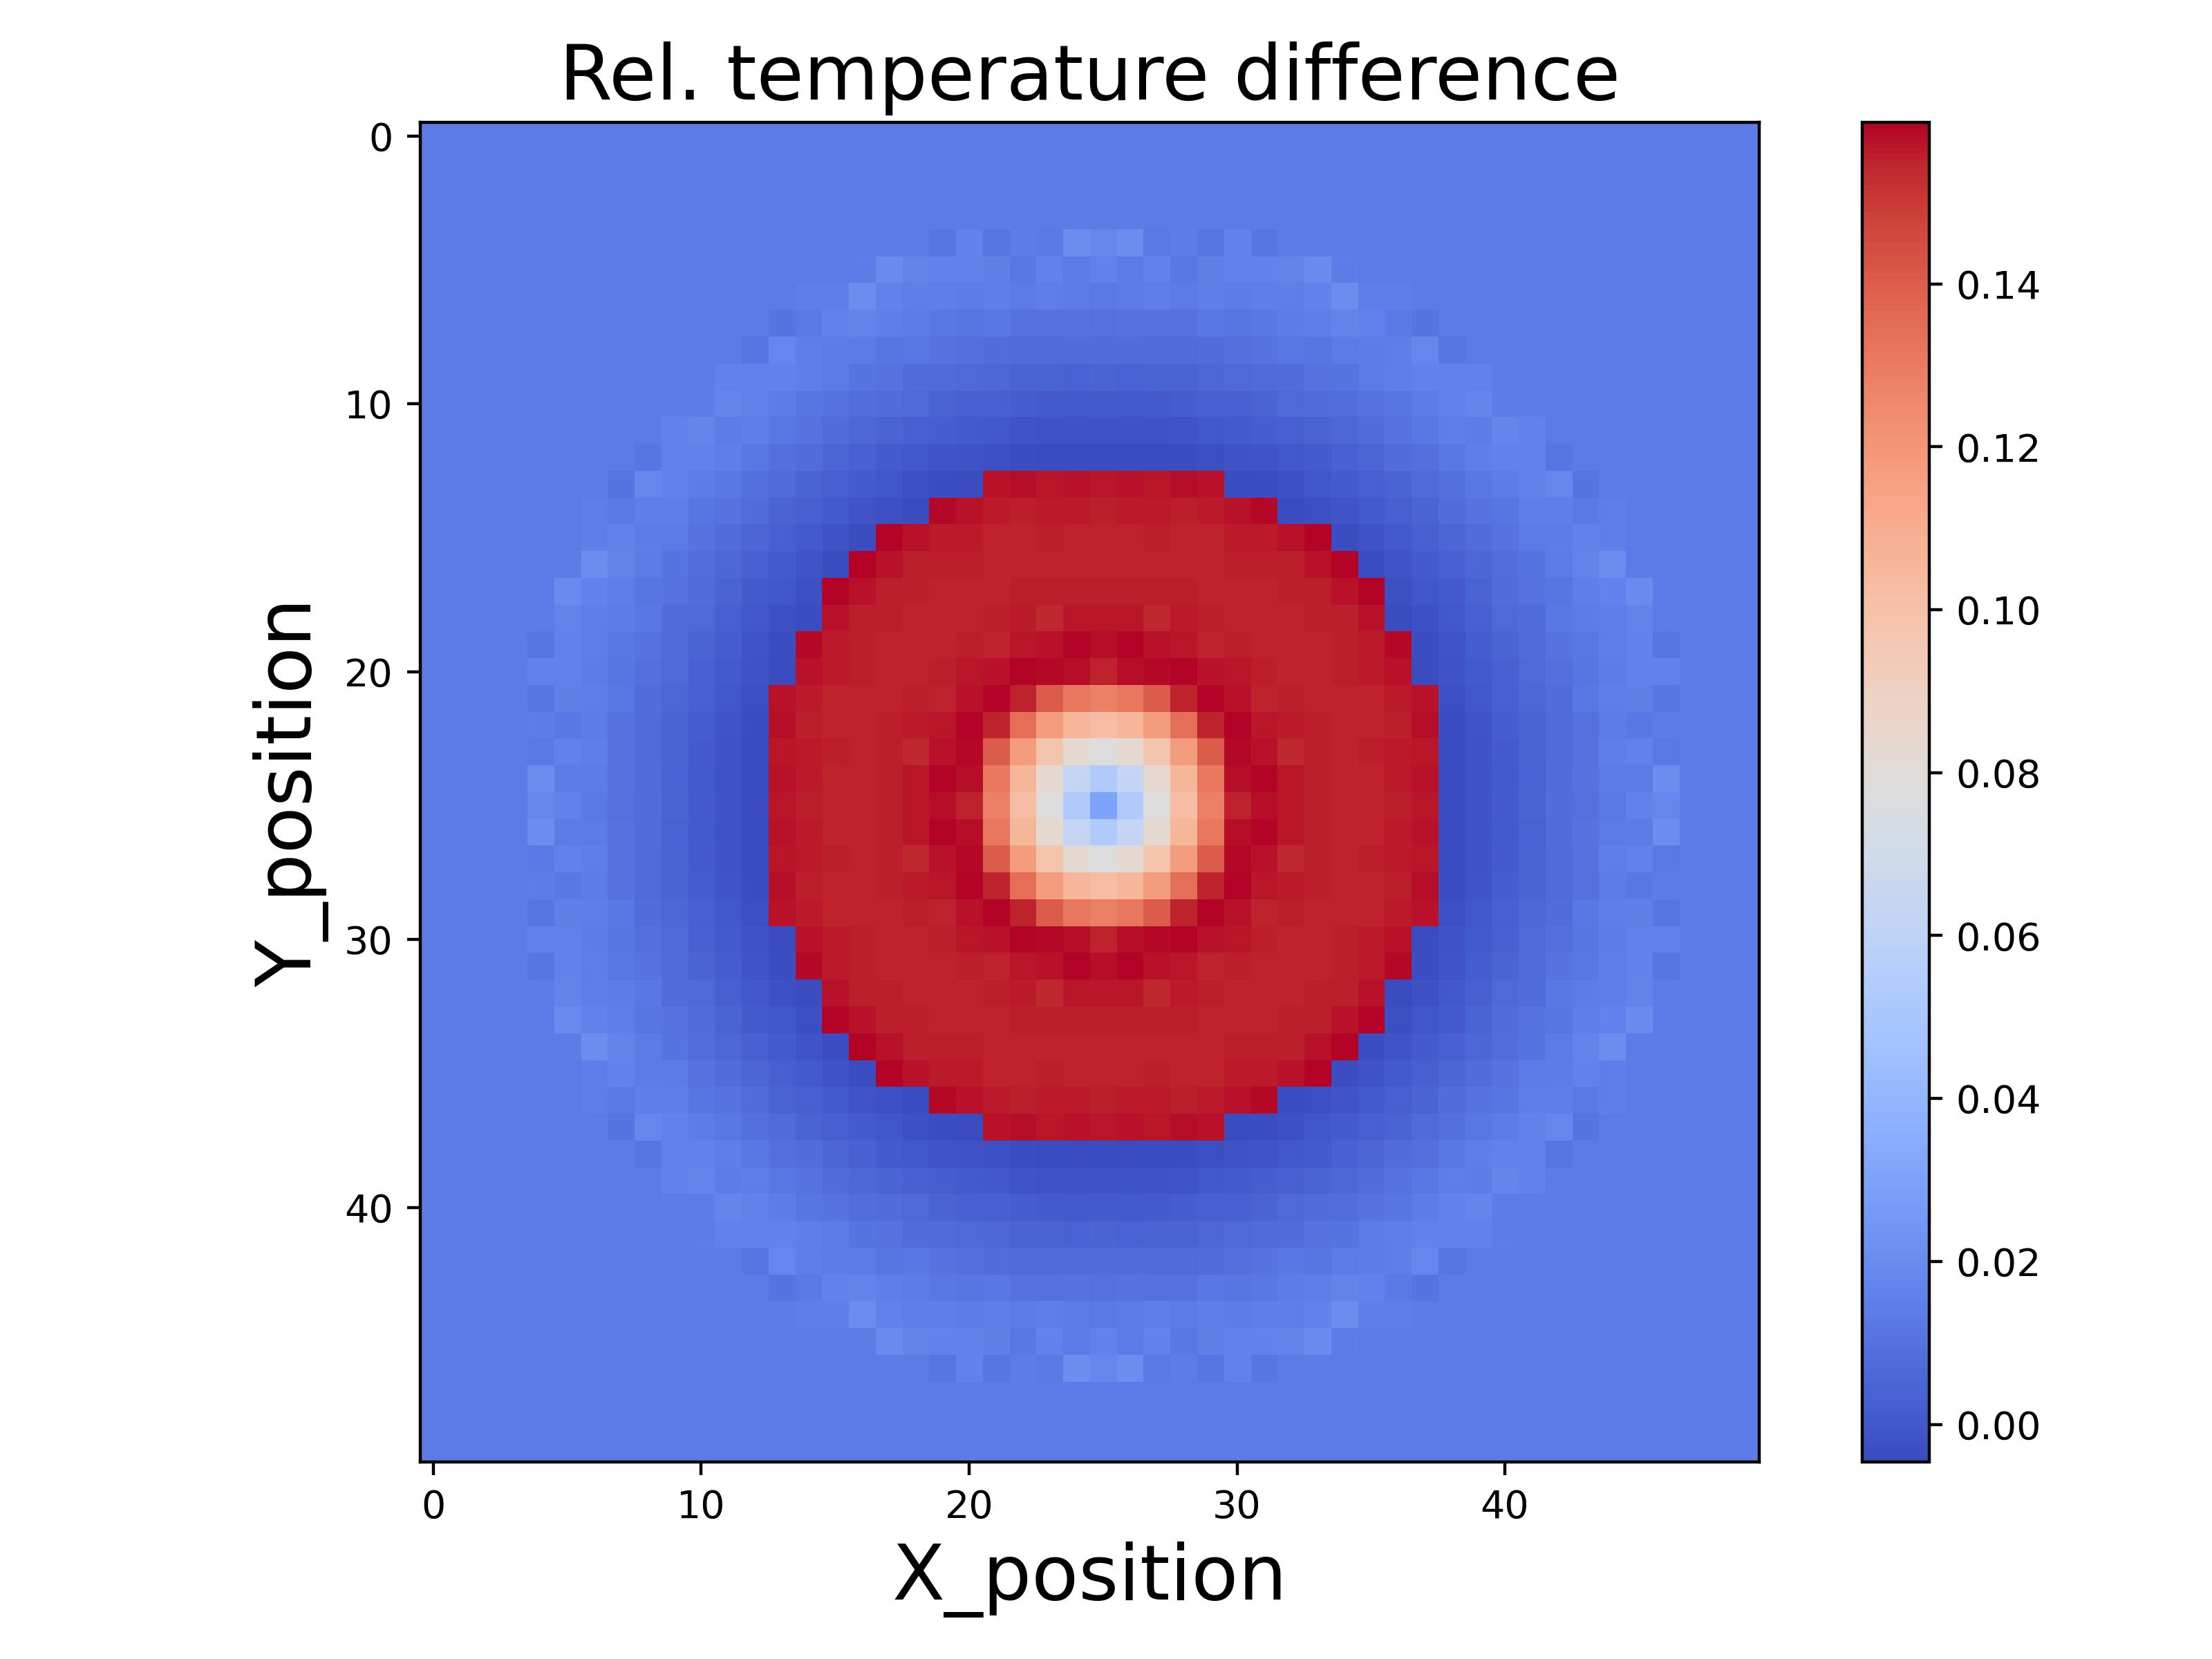
\includegraphics[width=\textwidth]{figures/raw_data/21/linear/T_bias.jpg}
            \subcaption{Model 1}
        \end{subfigure}
    \end{minipage}\\
    \begin{minipage}{\textwidth}
        \centering
        \begin{subfigure}{0.325\textwidth}
            \centering
            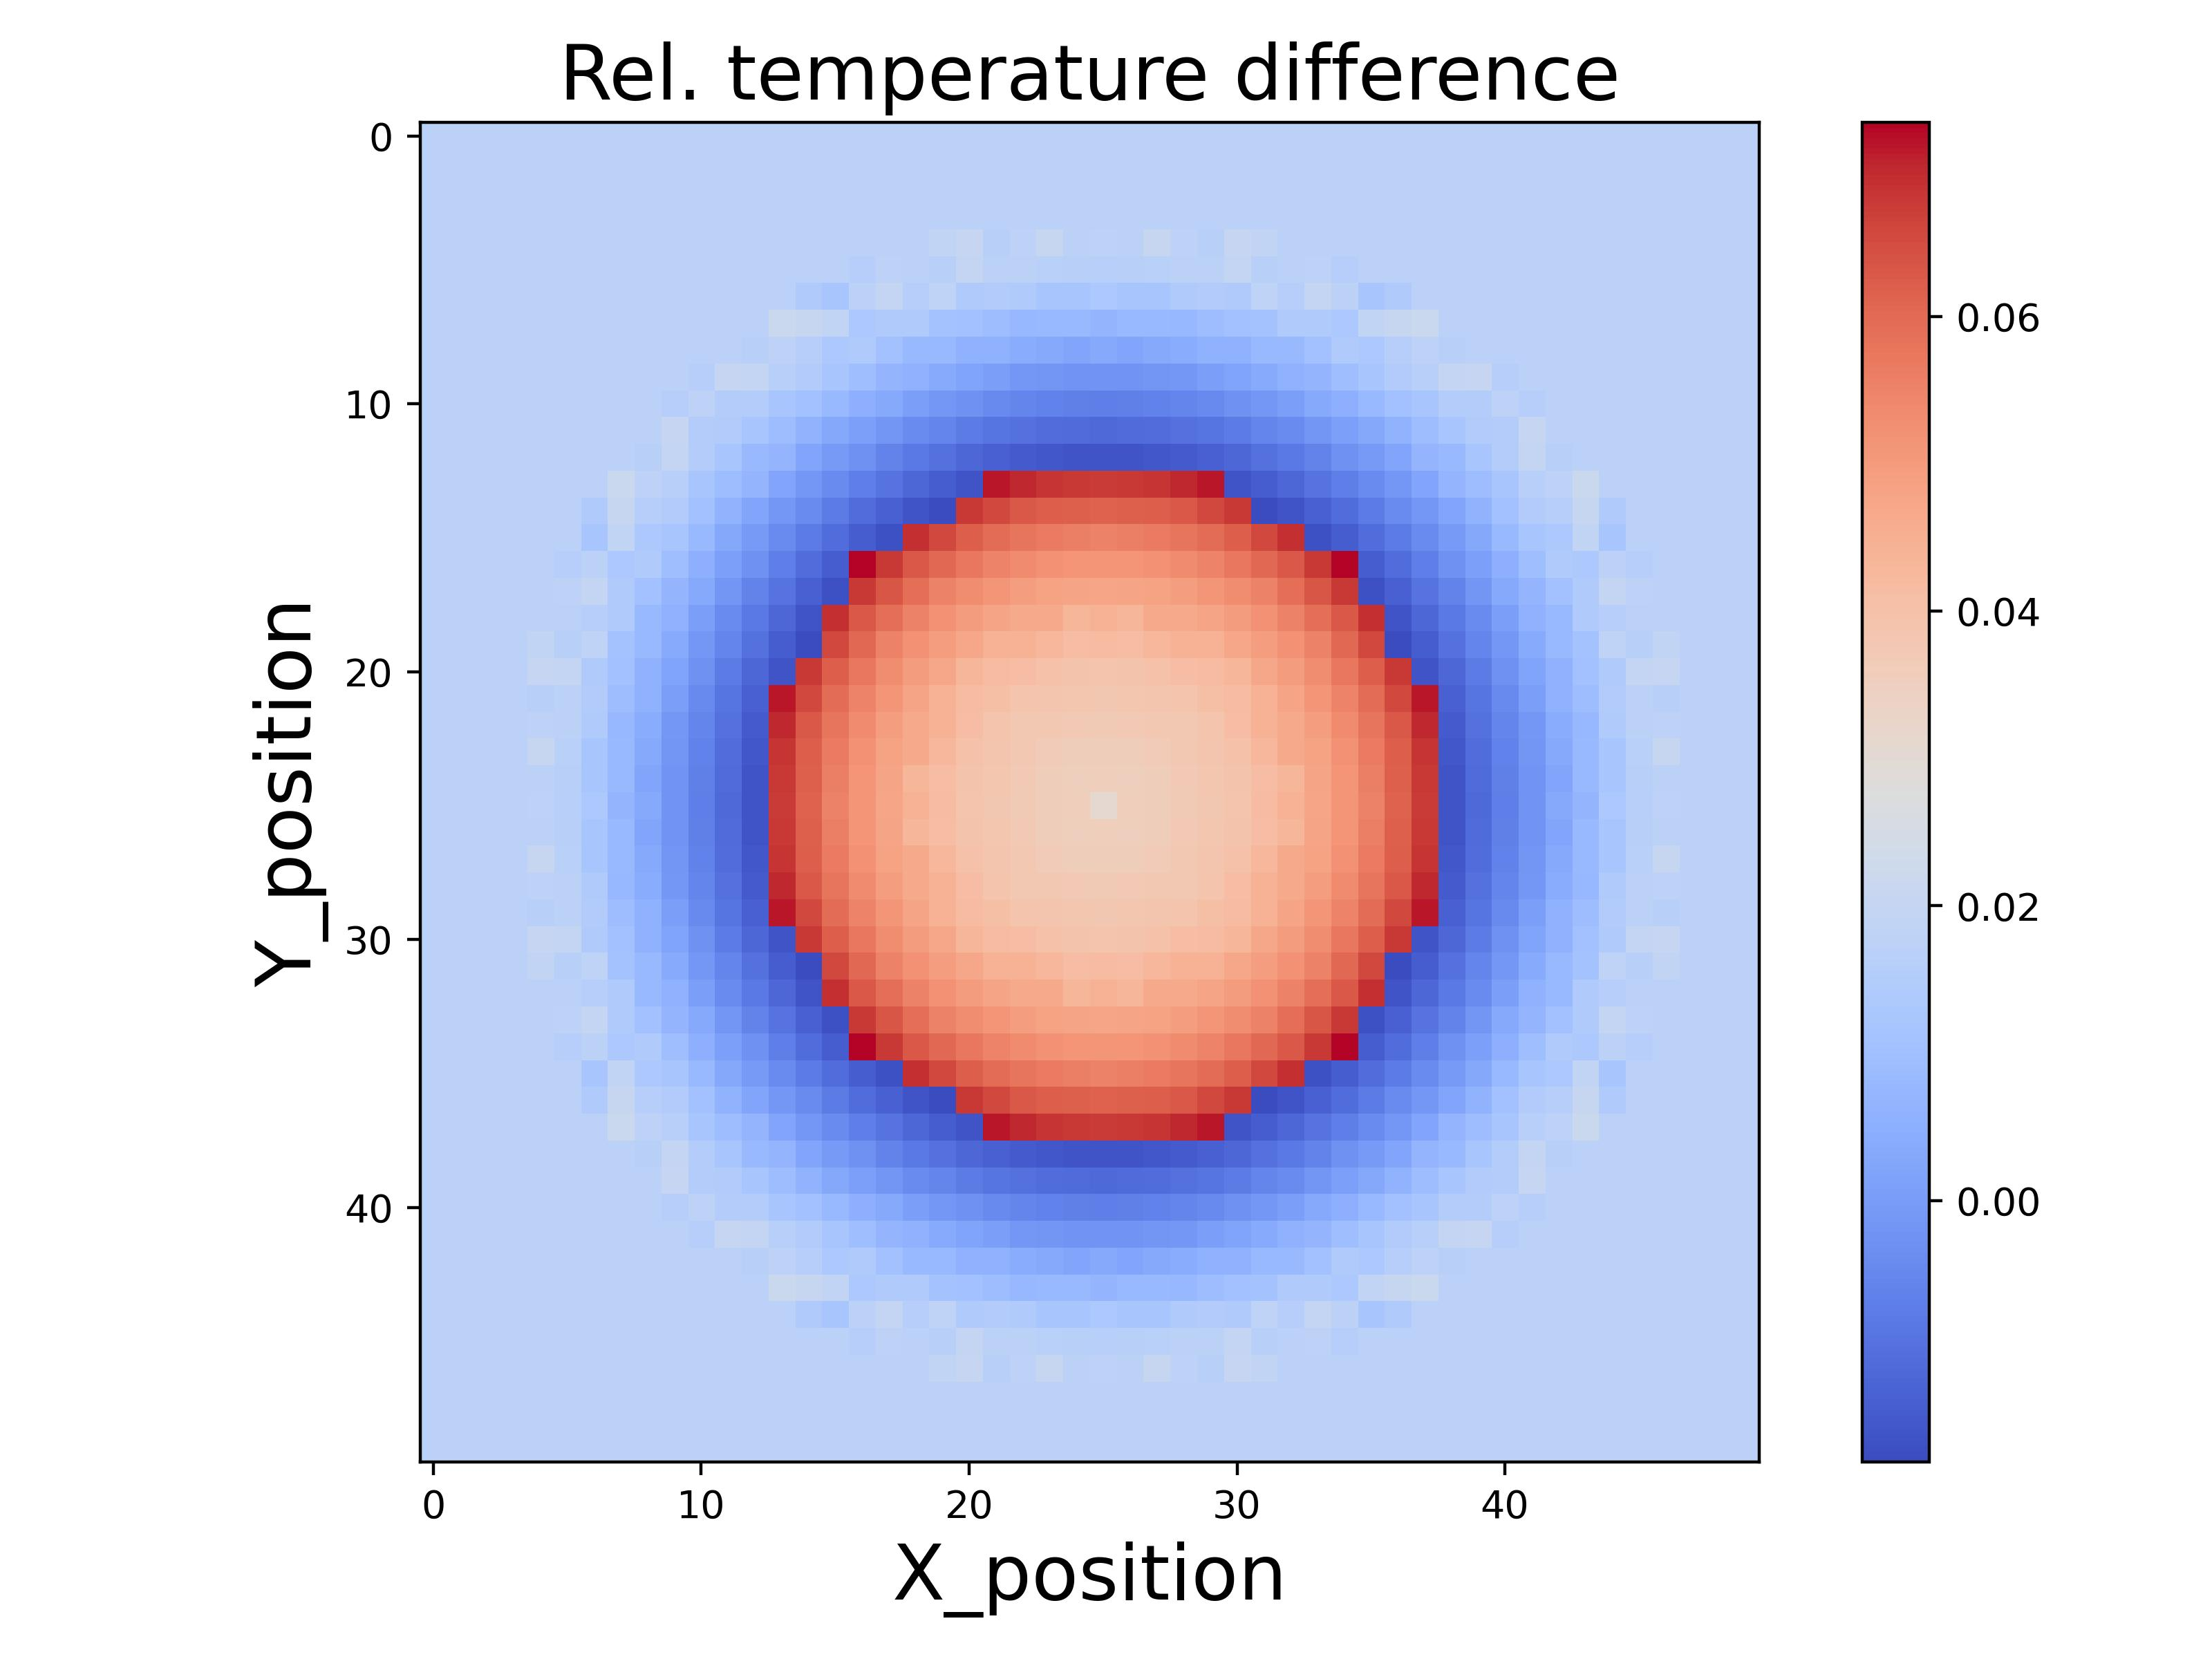
\includegraphics[width=\textwidth]{figures/raw_data/22/linear/T_bias.jpg}
            \subcaption{Model 2}
        \end{subfigure}
        \begin{subfigure}{0.325\textwidth}
            \centering
            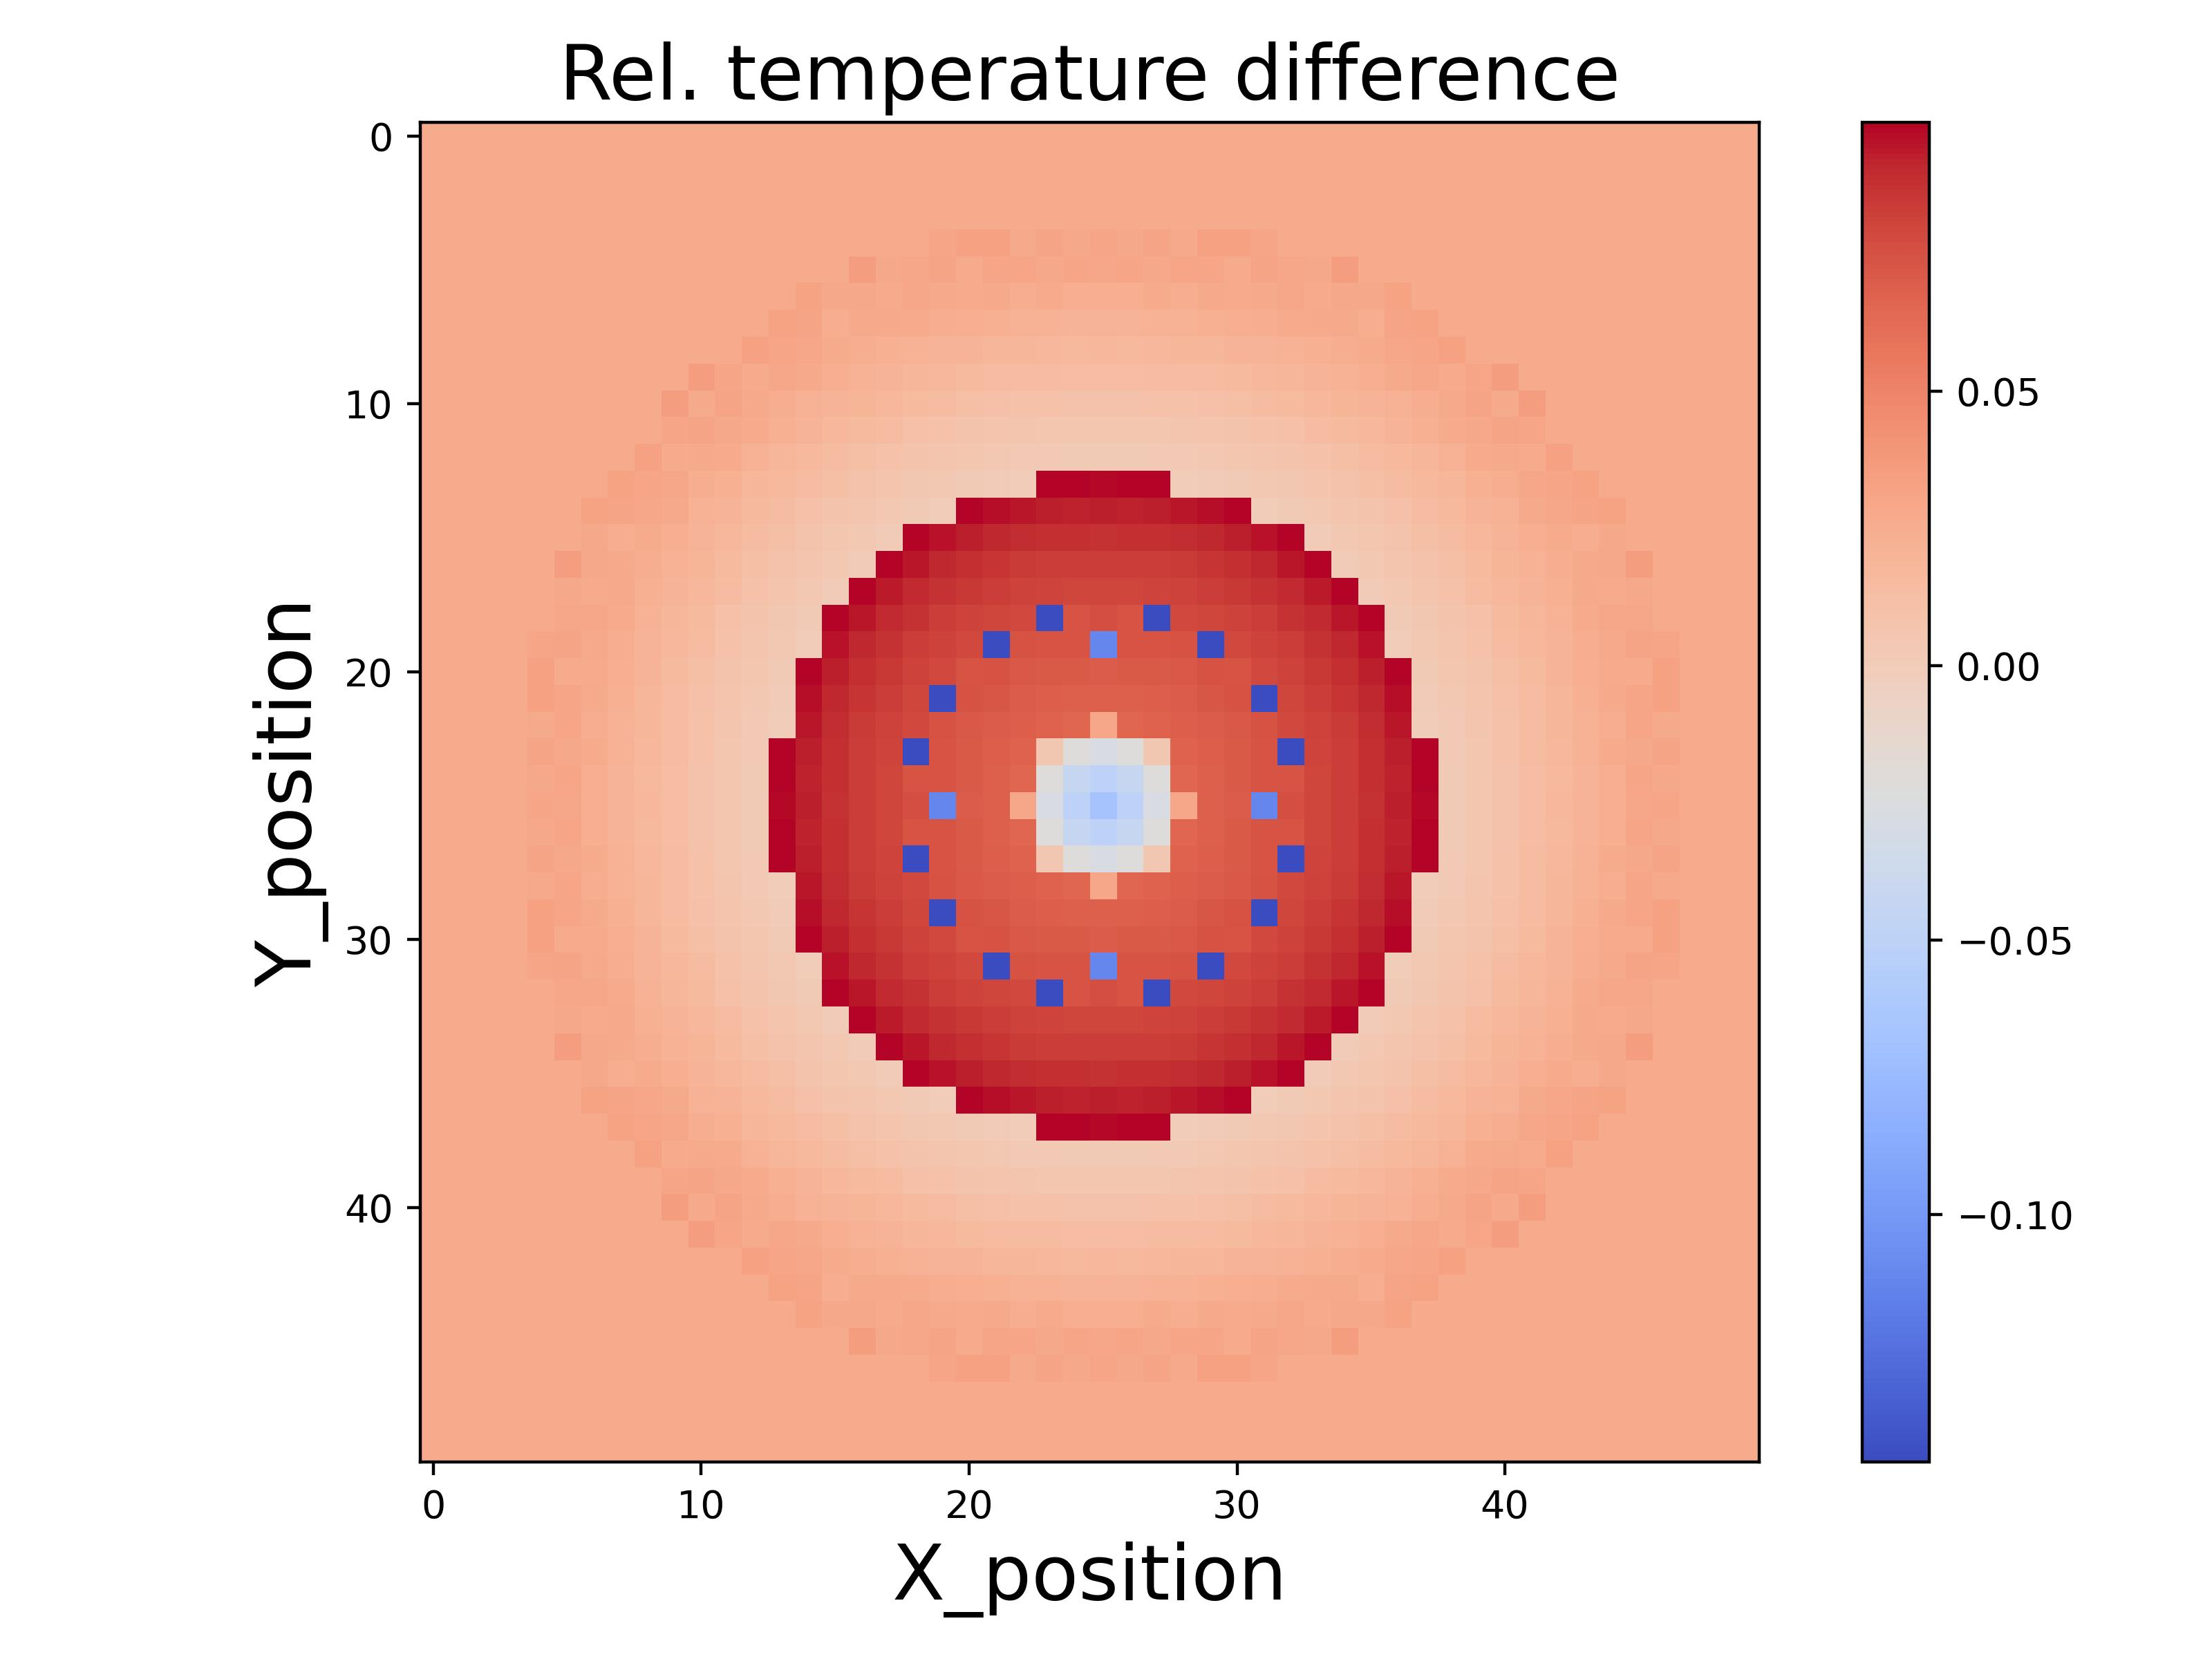
\includegraphics[width=\textwidth]{figures/raw_data/23/linear/T_bias.jpg}
            \subcaption{Model 3}
        \end{subfigure}
        \begin{subfigure}{0.325\textwidth}
            \centering
            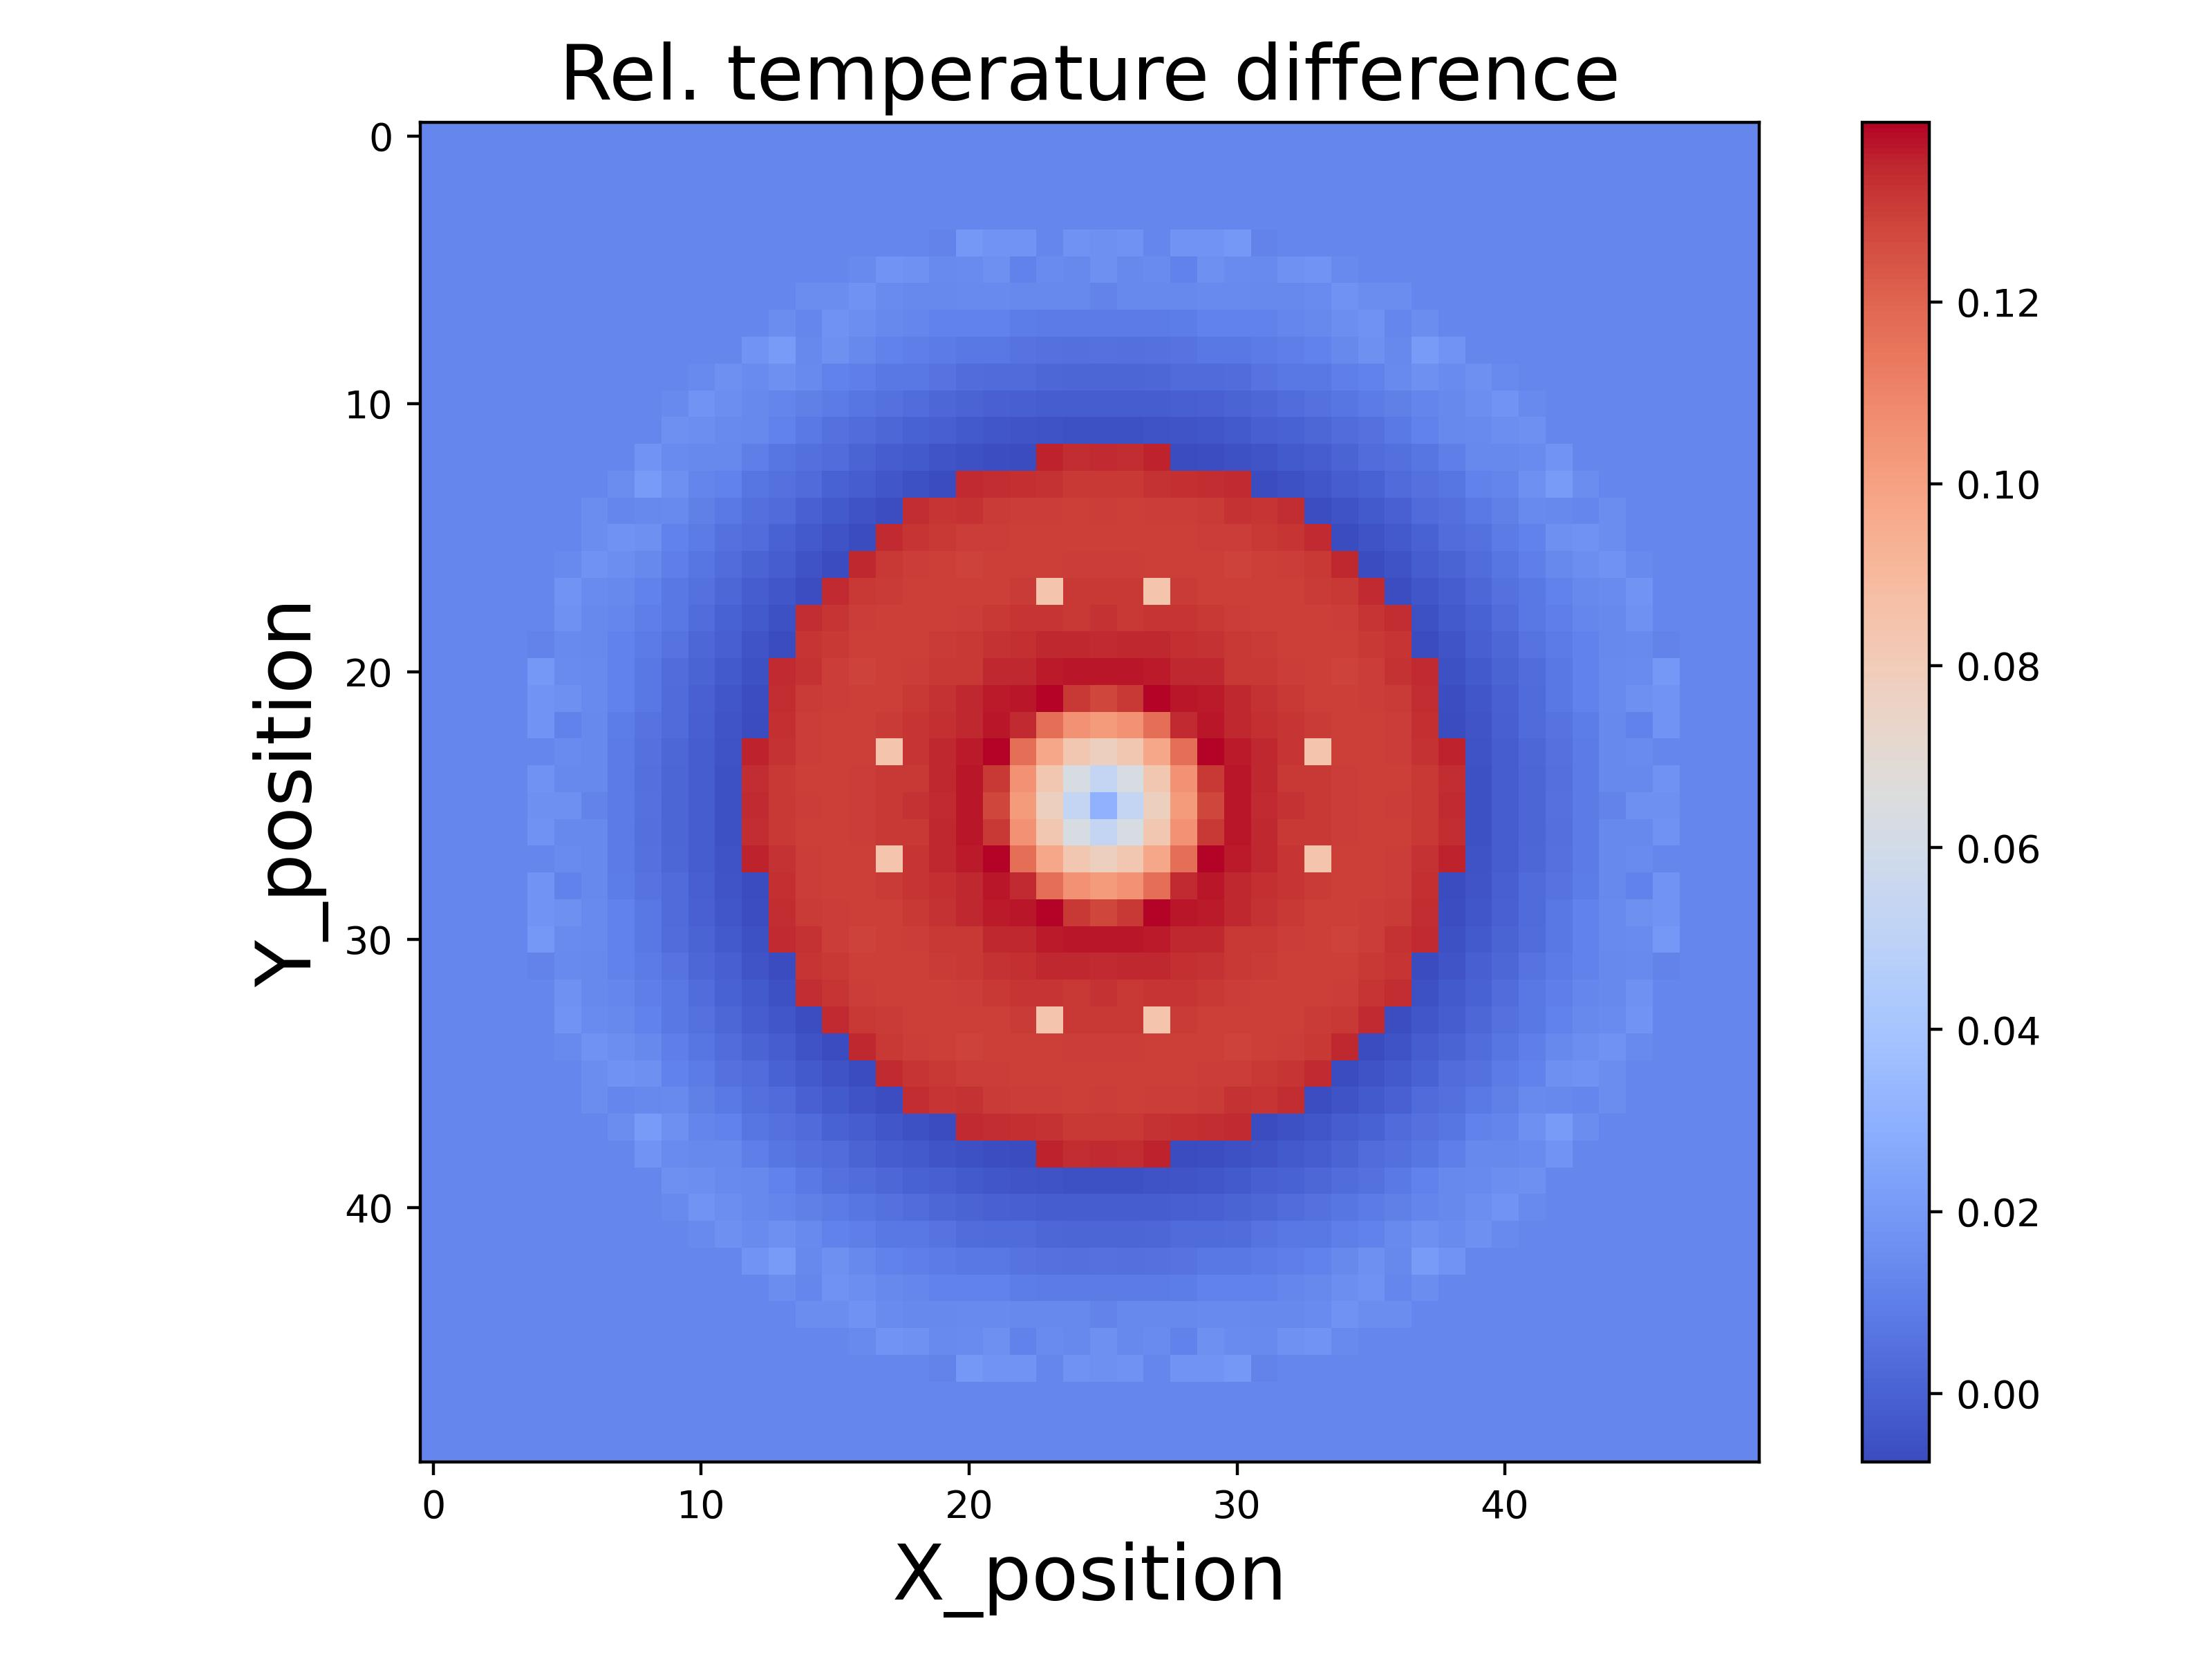
\includegraphics[width=\textwidth]{figures/raw_data/24/linear/T_bias.jpg}
            \subcaption{Model 4}
        \end{subfigure}
    \end{minipage}\\
    \begin{minipage}{\textwidth}
        \centering
        \begin{subfigure}{0.325\textwidth}
            \centering
            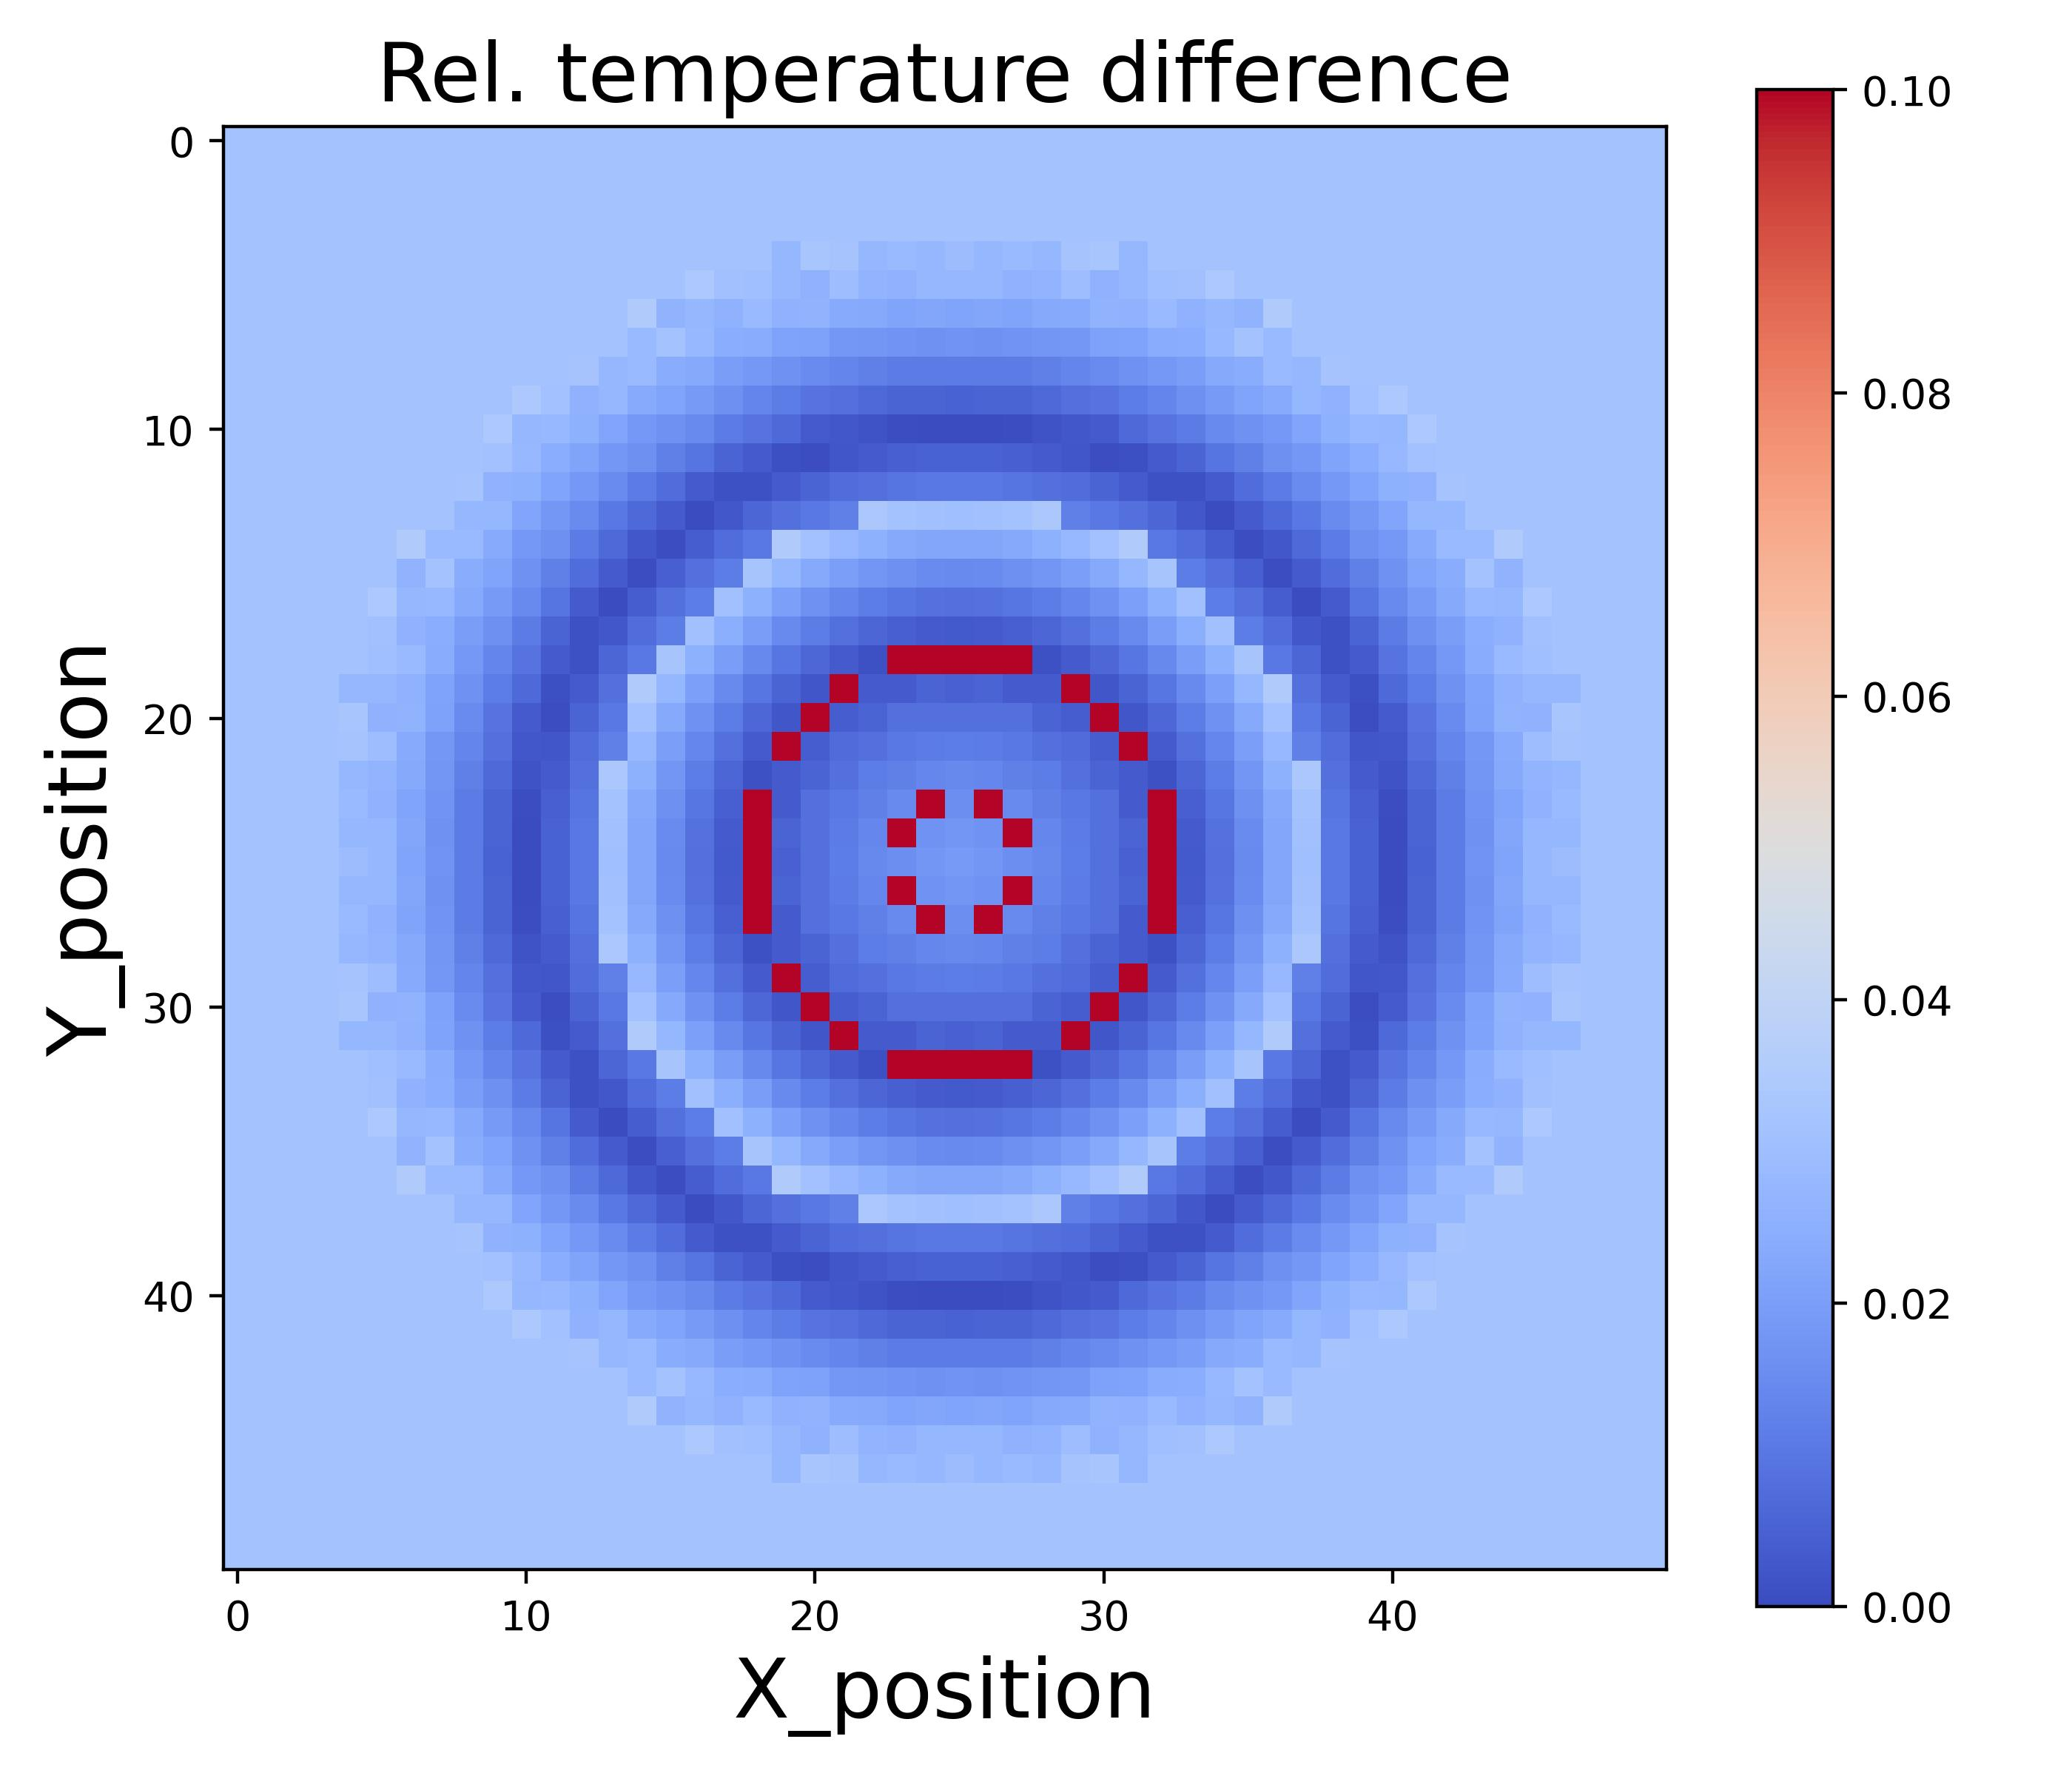
\includegraphics[width=\textwidth]{figures/raw_data/25/linear/T_bias.jpg}
            \subcaption{Model 5}
        \end{subfigure}
        \begin{subfigure}{0.325\textwidth}
            \centering
            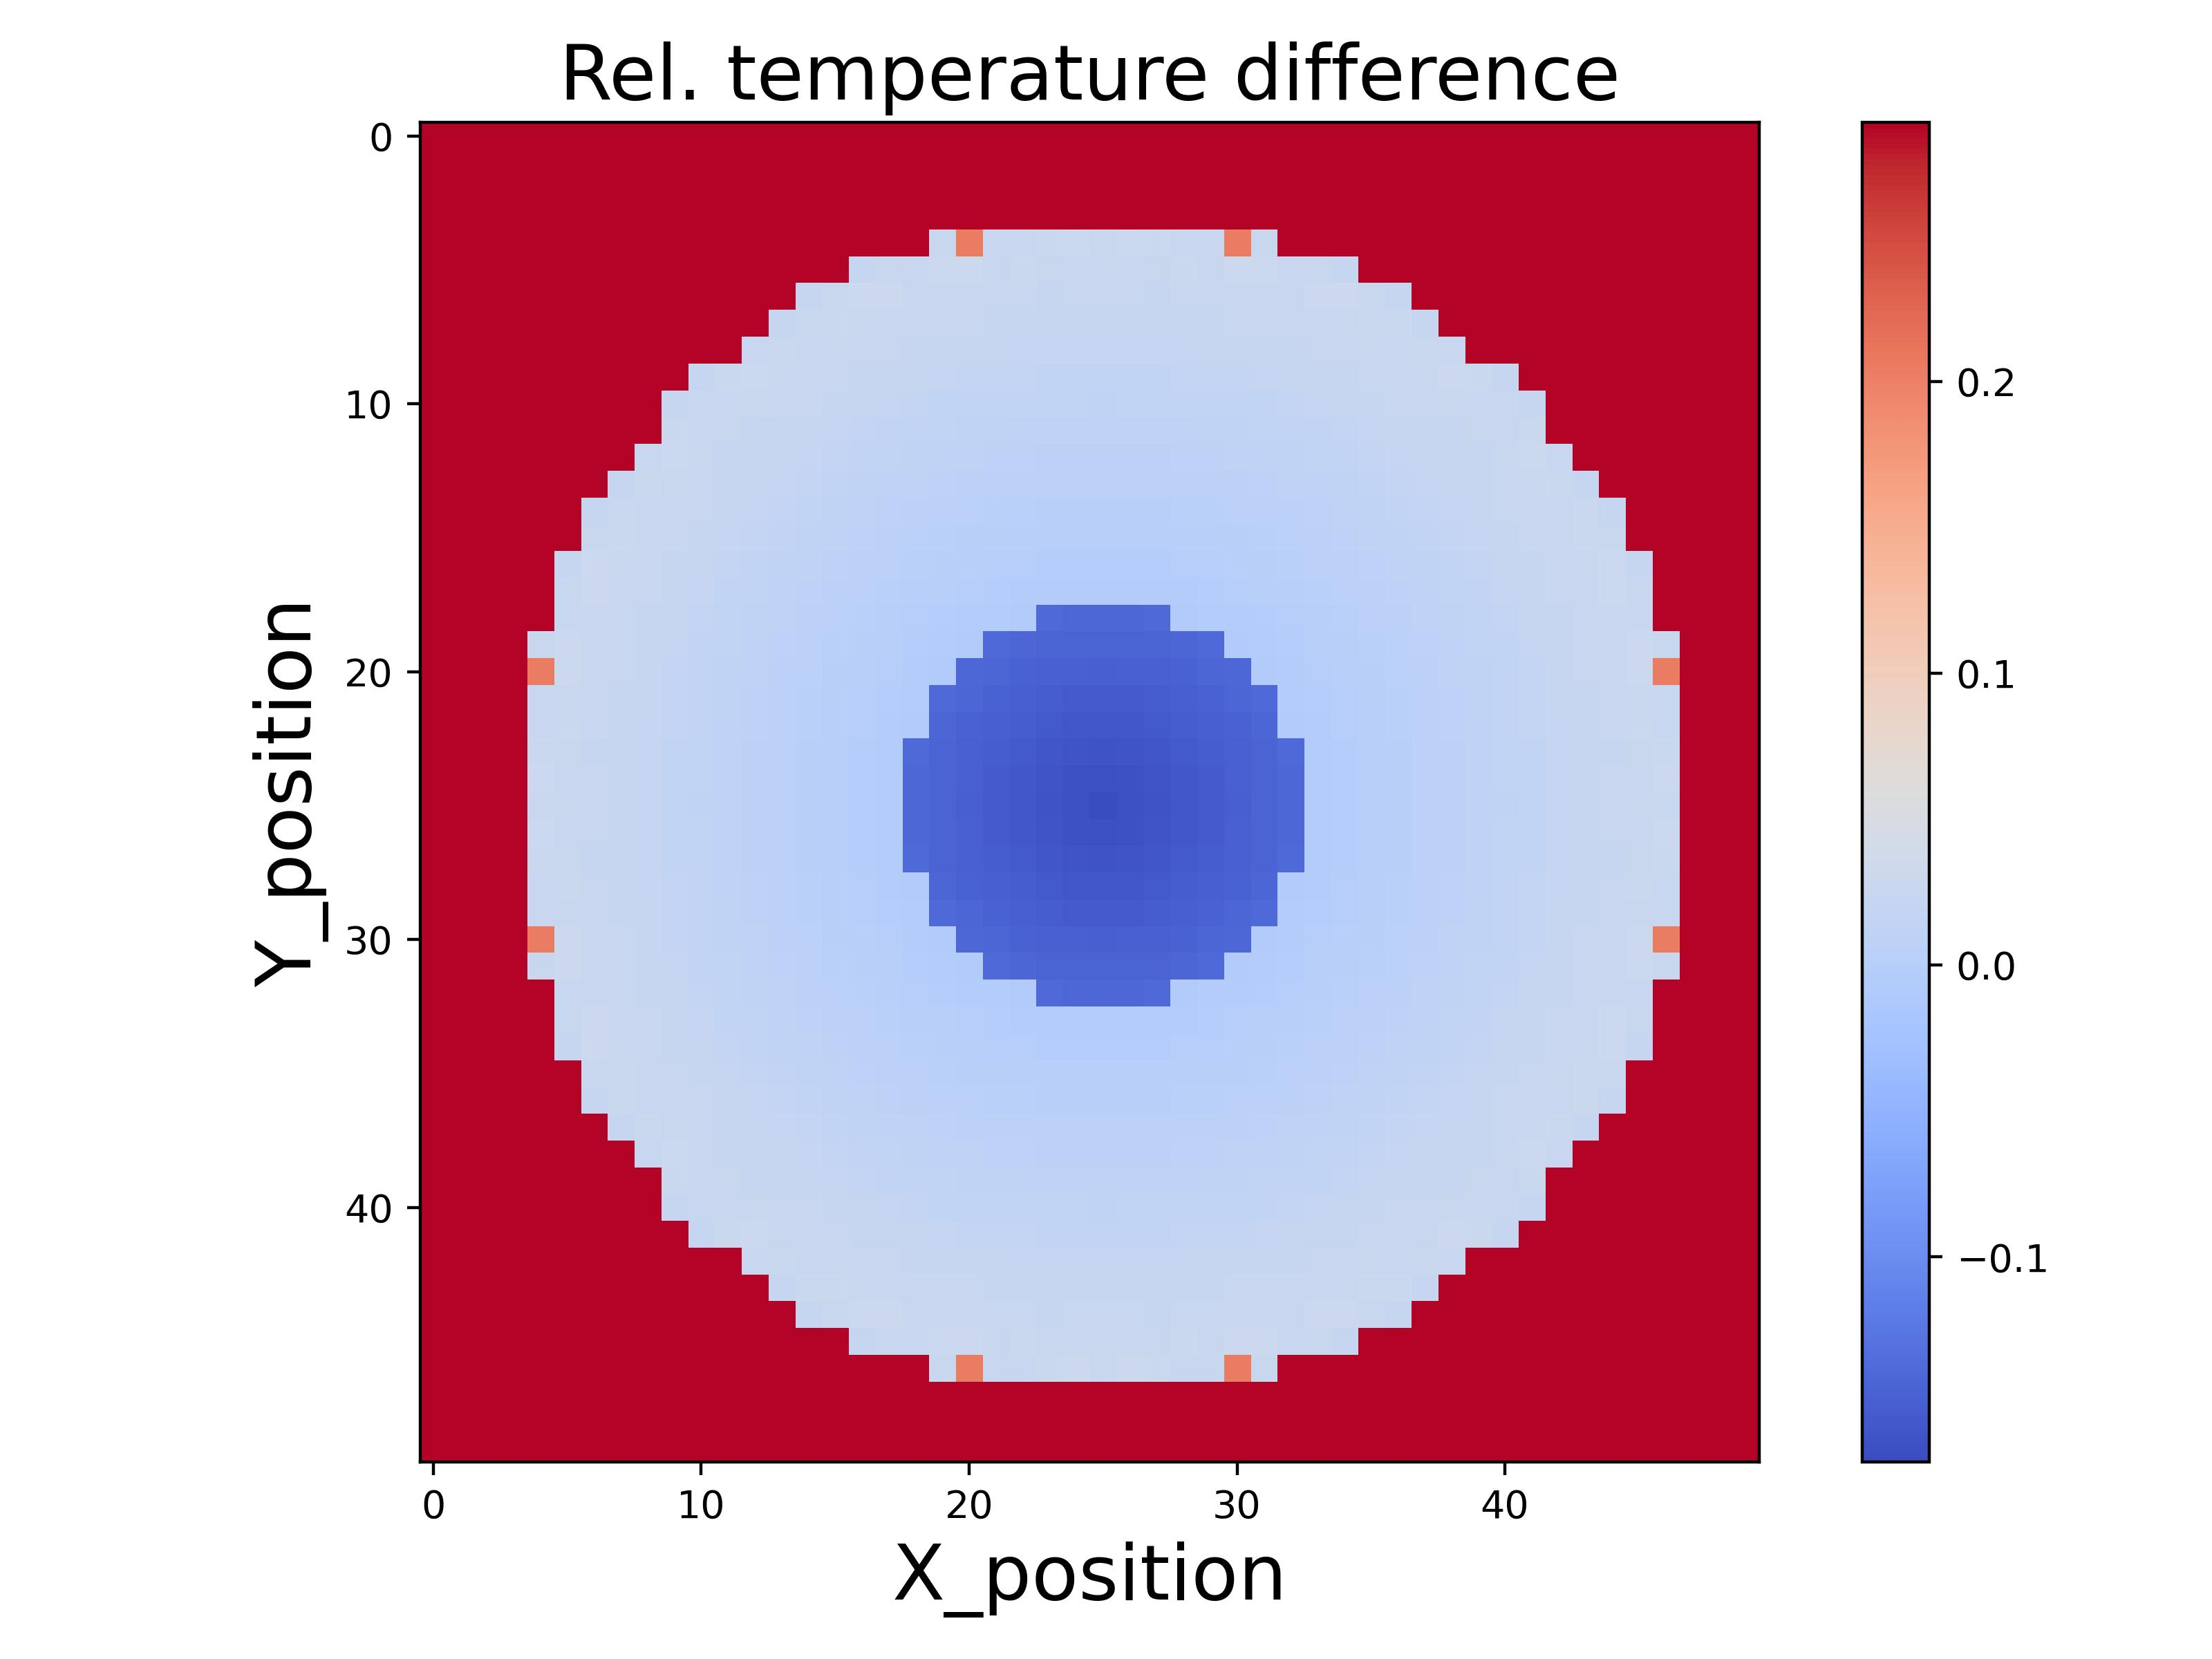
\includegraphics[width=\textwidth]{figures/raw_data/26/linear/T_bias.jpg}
            \subcaption{Model 6}
        \end{subfigure}
        \begin{subfigure}{0.325\textwidth}
            \centering
            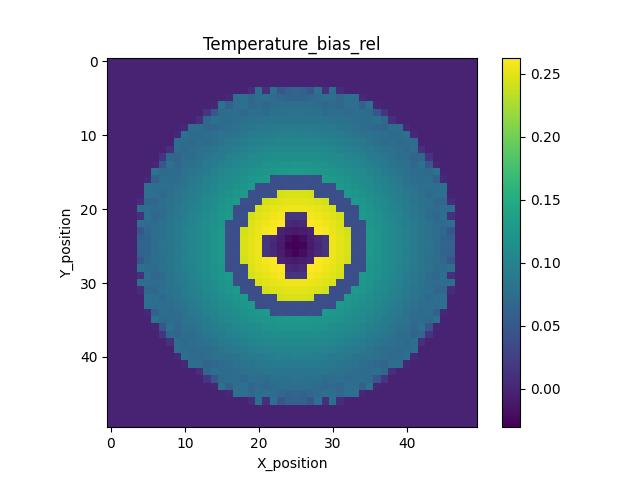
\includegraphics[width=\textwidth]{figures/raw_data/31/linear/T_bias.jpg}
            \subcaption{Model 7}
        \end{subfigure}
    \end{minipage}\\
    \begin{minipage}{\textwidth}
        \centering
        \begin{subfigure}{0.325\textwidth}
            \centering
            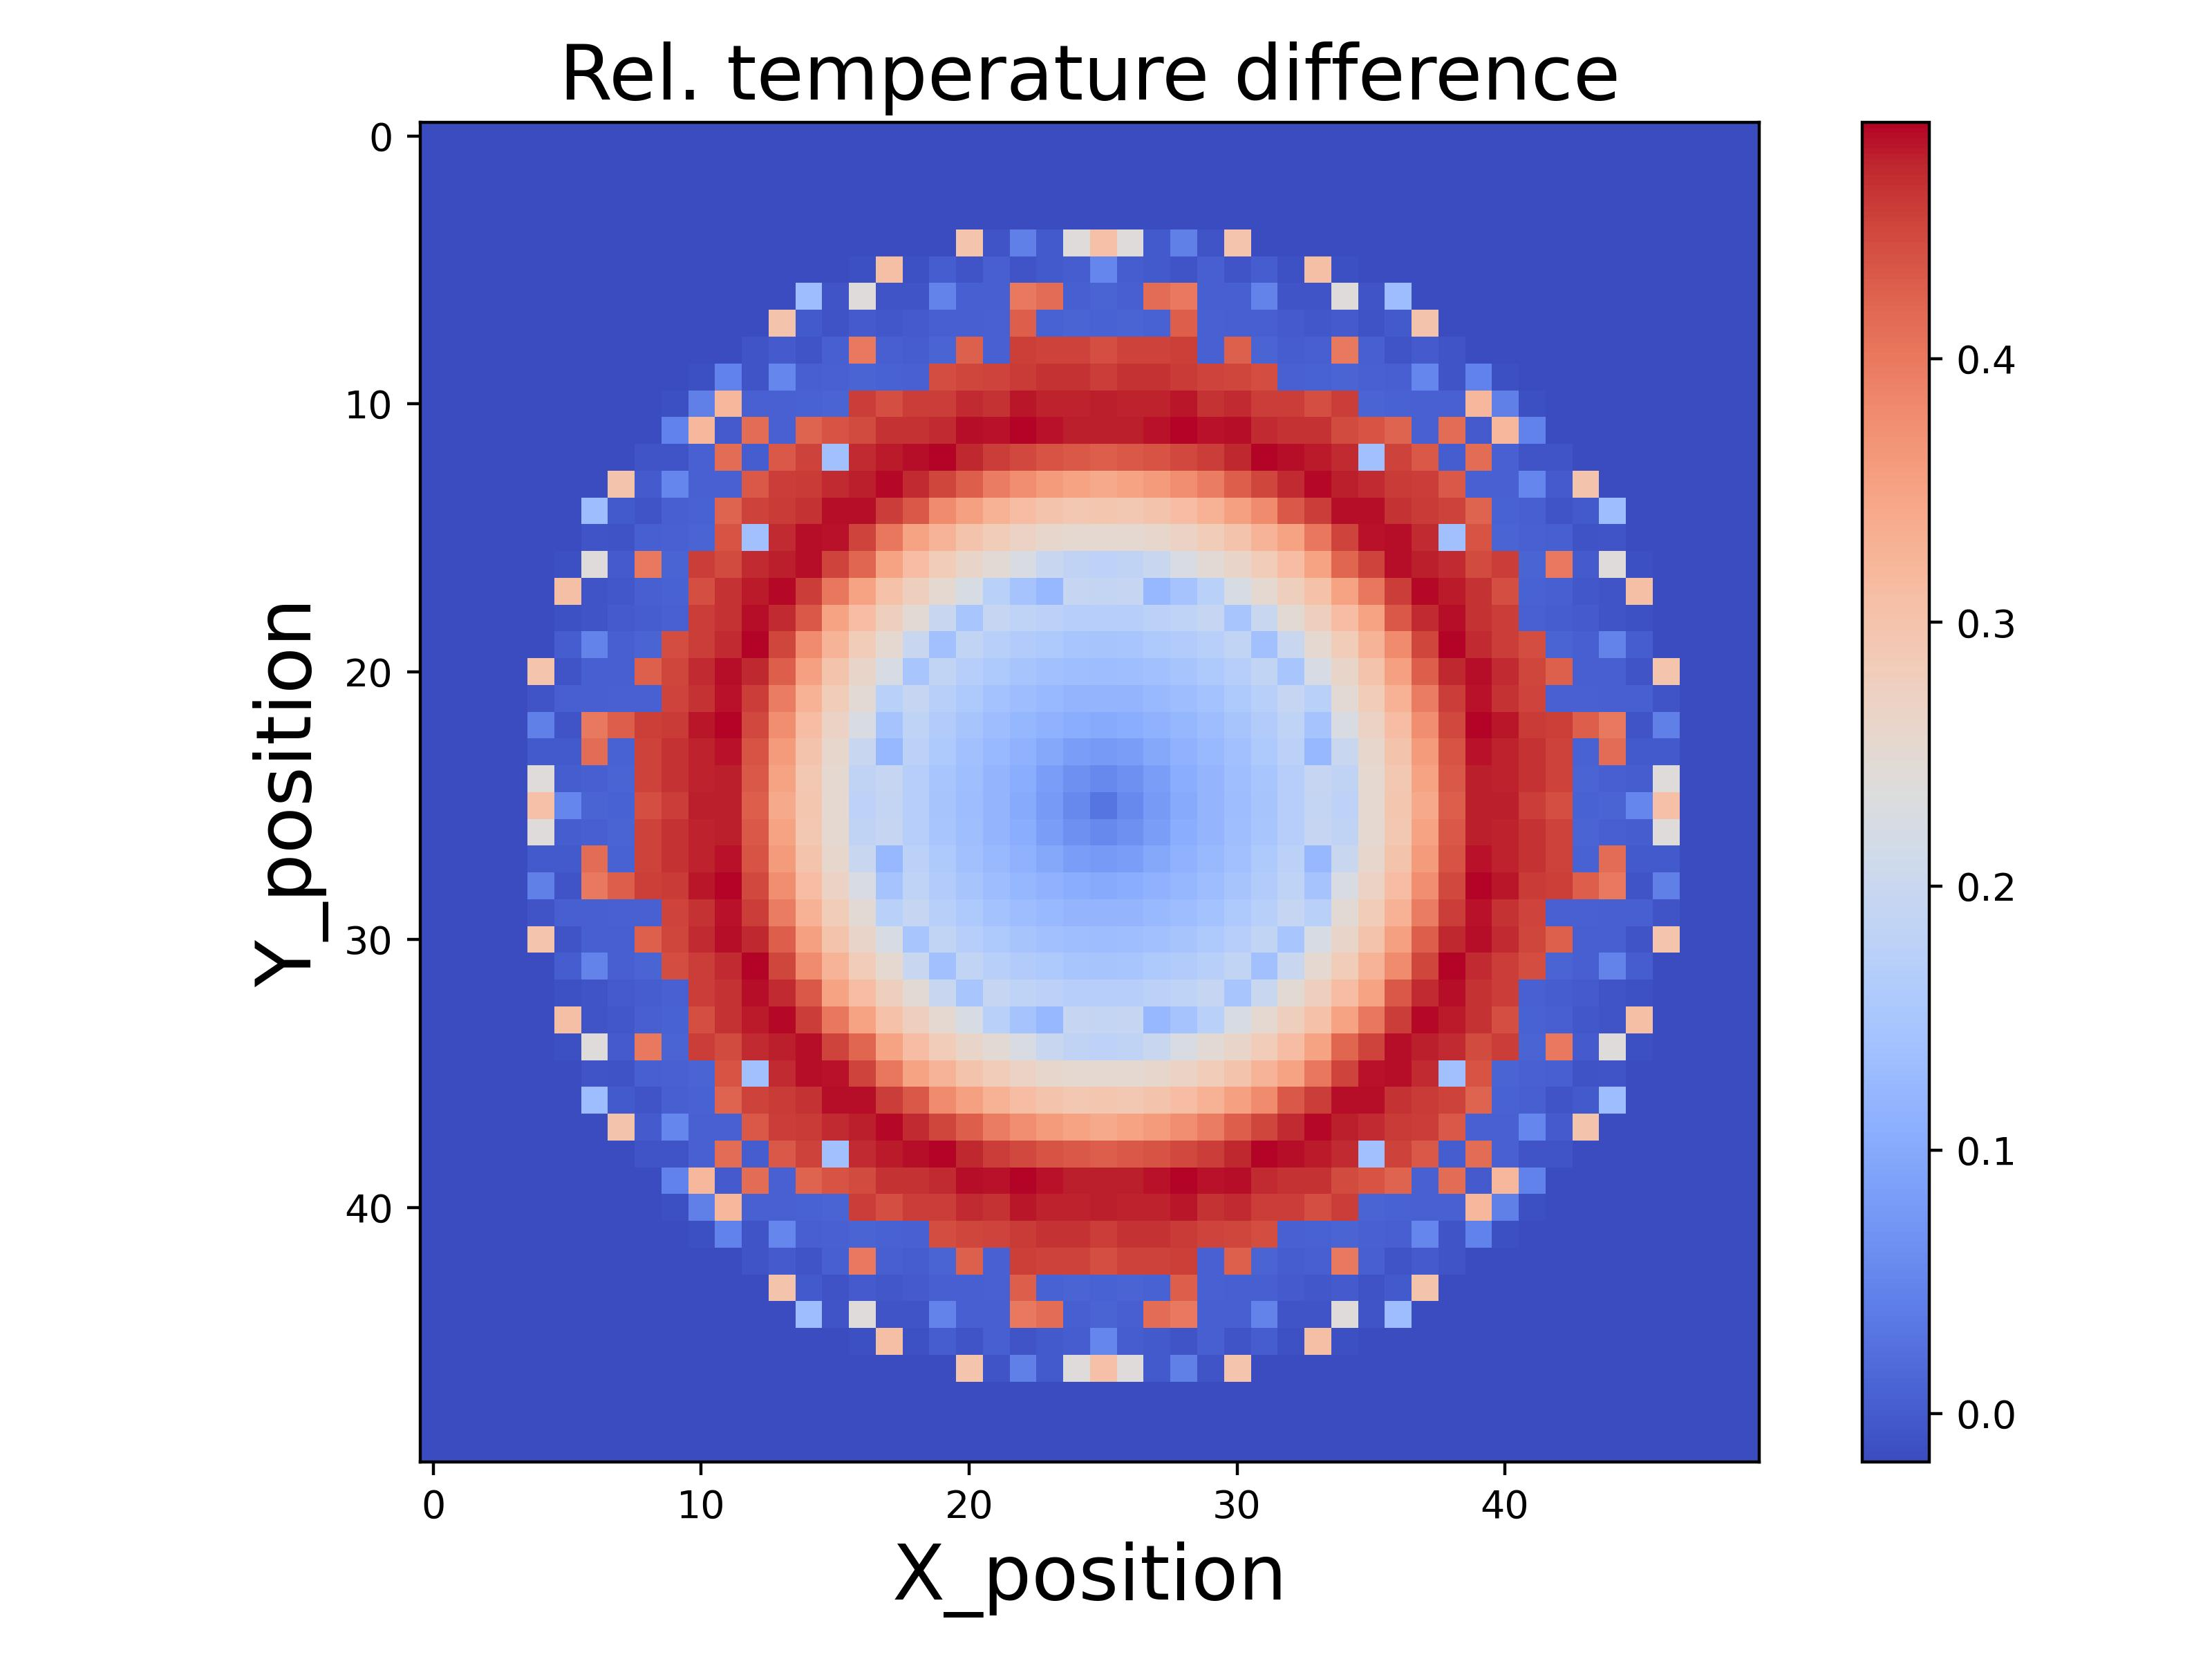
\includegraphics[width=\textwidth]{figures/raw_data/32/linear/T_bias.jpg}
            \subcaption{Model 8}
        \end{subfigure}
        \begin{subfigure}{0.325\textwidth}
            \centering
            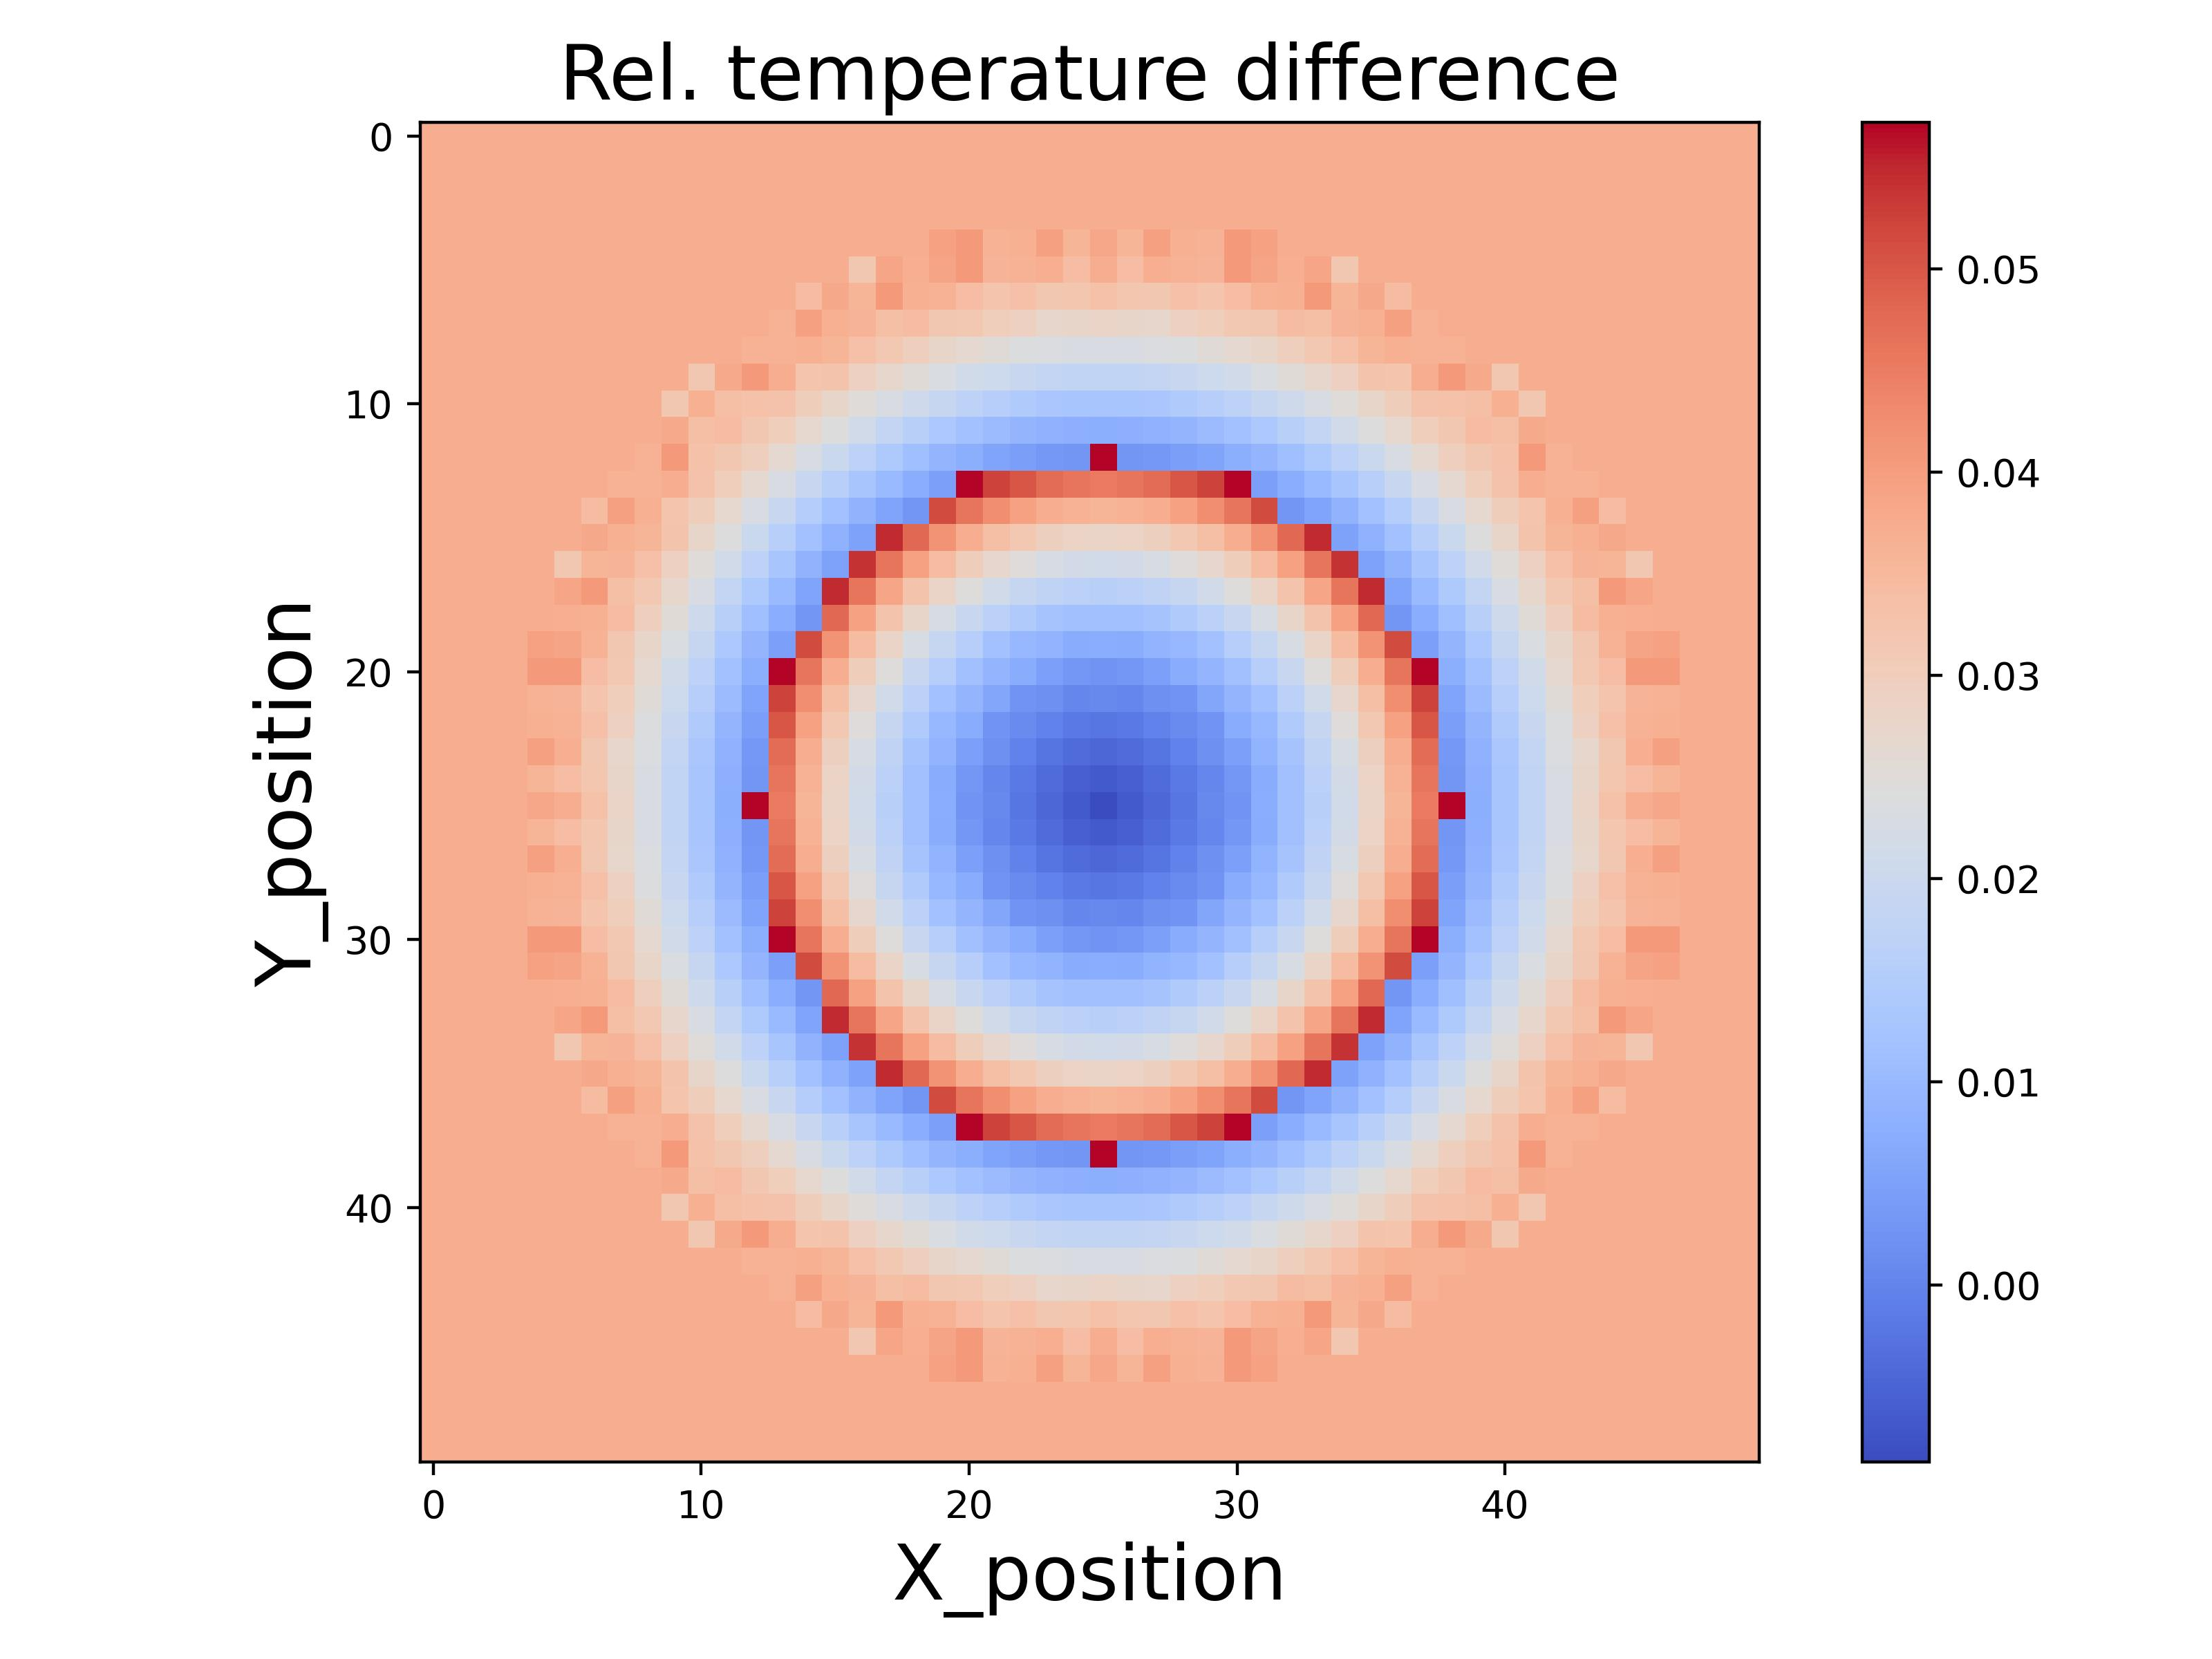
\includegraphics[width=\textwidth]{figures/raw_data/33/linear/T_bias.jpg}
            \subcaption{Model 9}
        \end{subfigure}
    \end{minipage}
    \caption{Temperature calculation results of mixed model}  
\end{figure}
\begin{figure}[p]
    \centering
    \begin{minipage}{\textwidth}
        \centering
        \begin{subfigure}{0.325\textwidth}
            \centering
            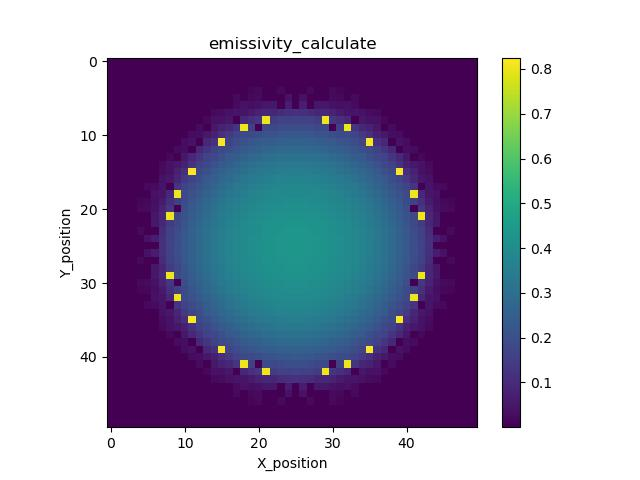
\includegraphics[width=\textwidth]{figures/raw_data/0/linear/emi_cal.jpg}
            \subcaption{Black body material}
        \end{subfigure}
        \begin{subfigure}{0.325\textwidth}
            \centering
            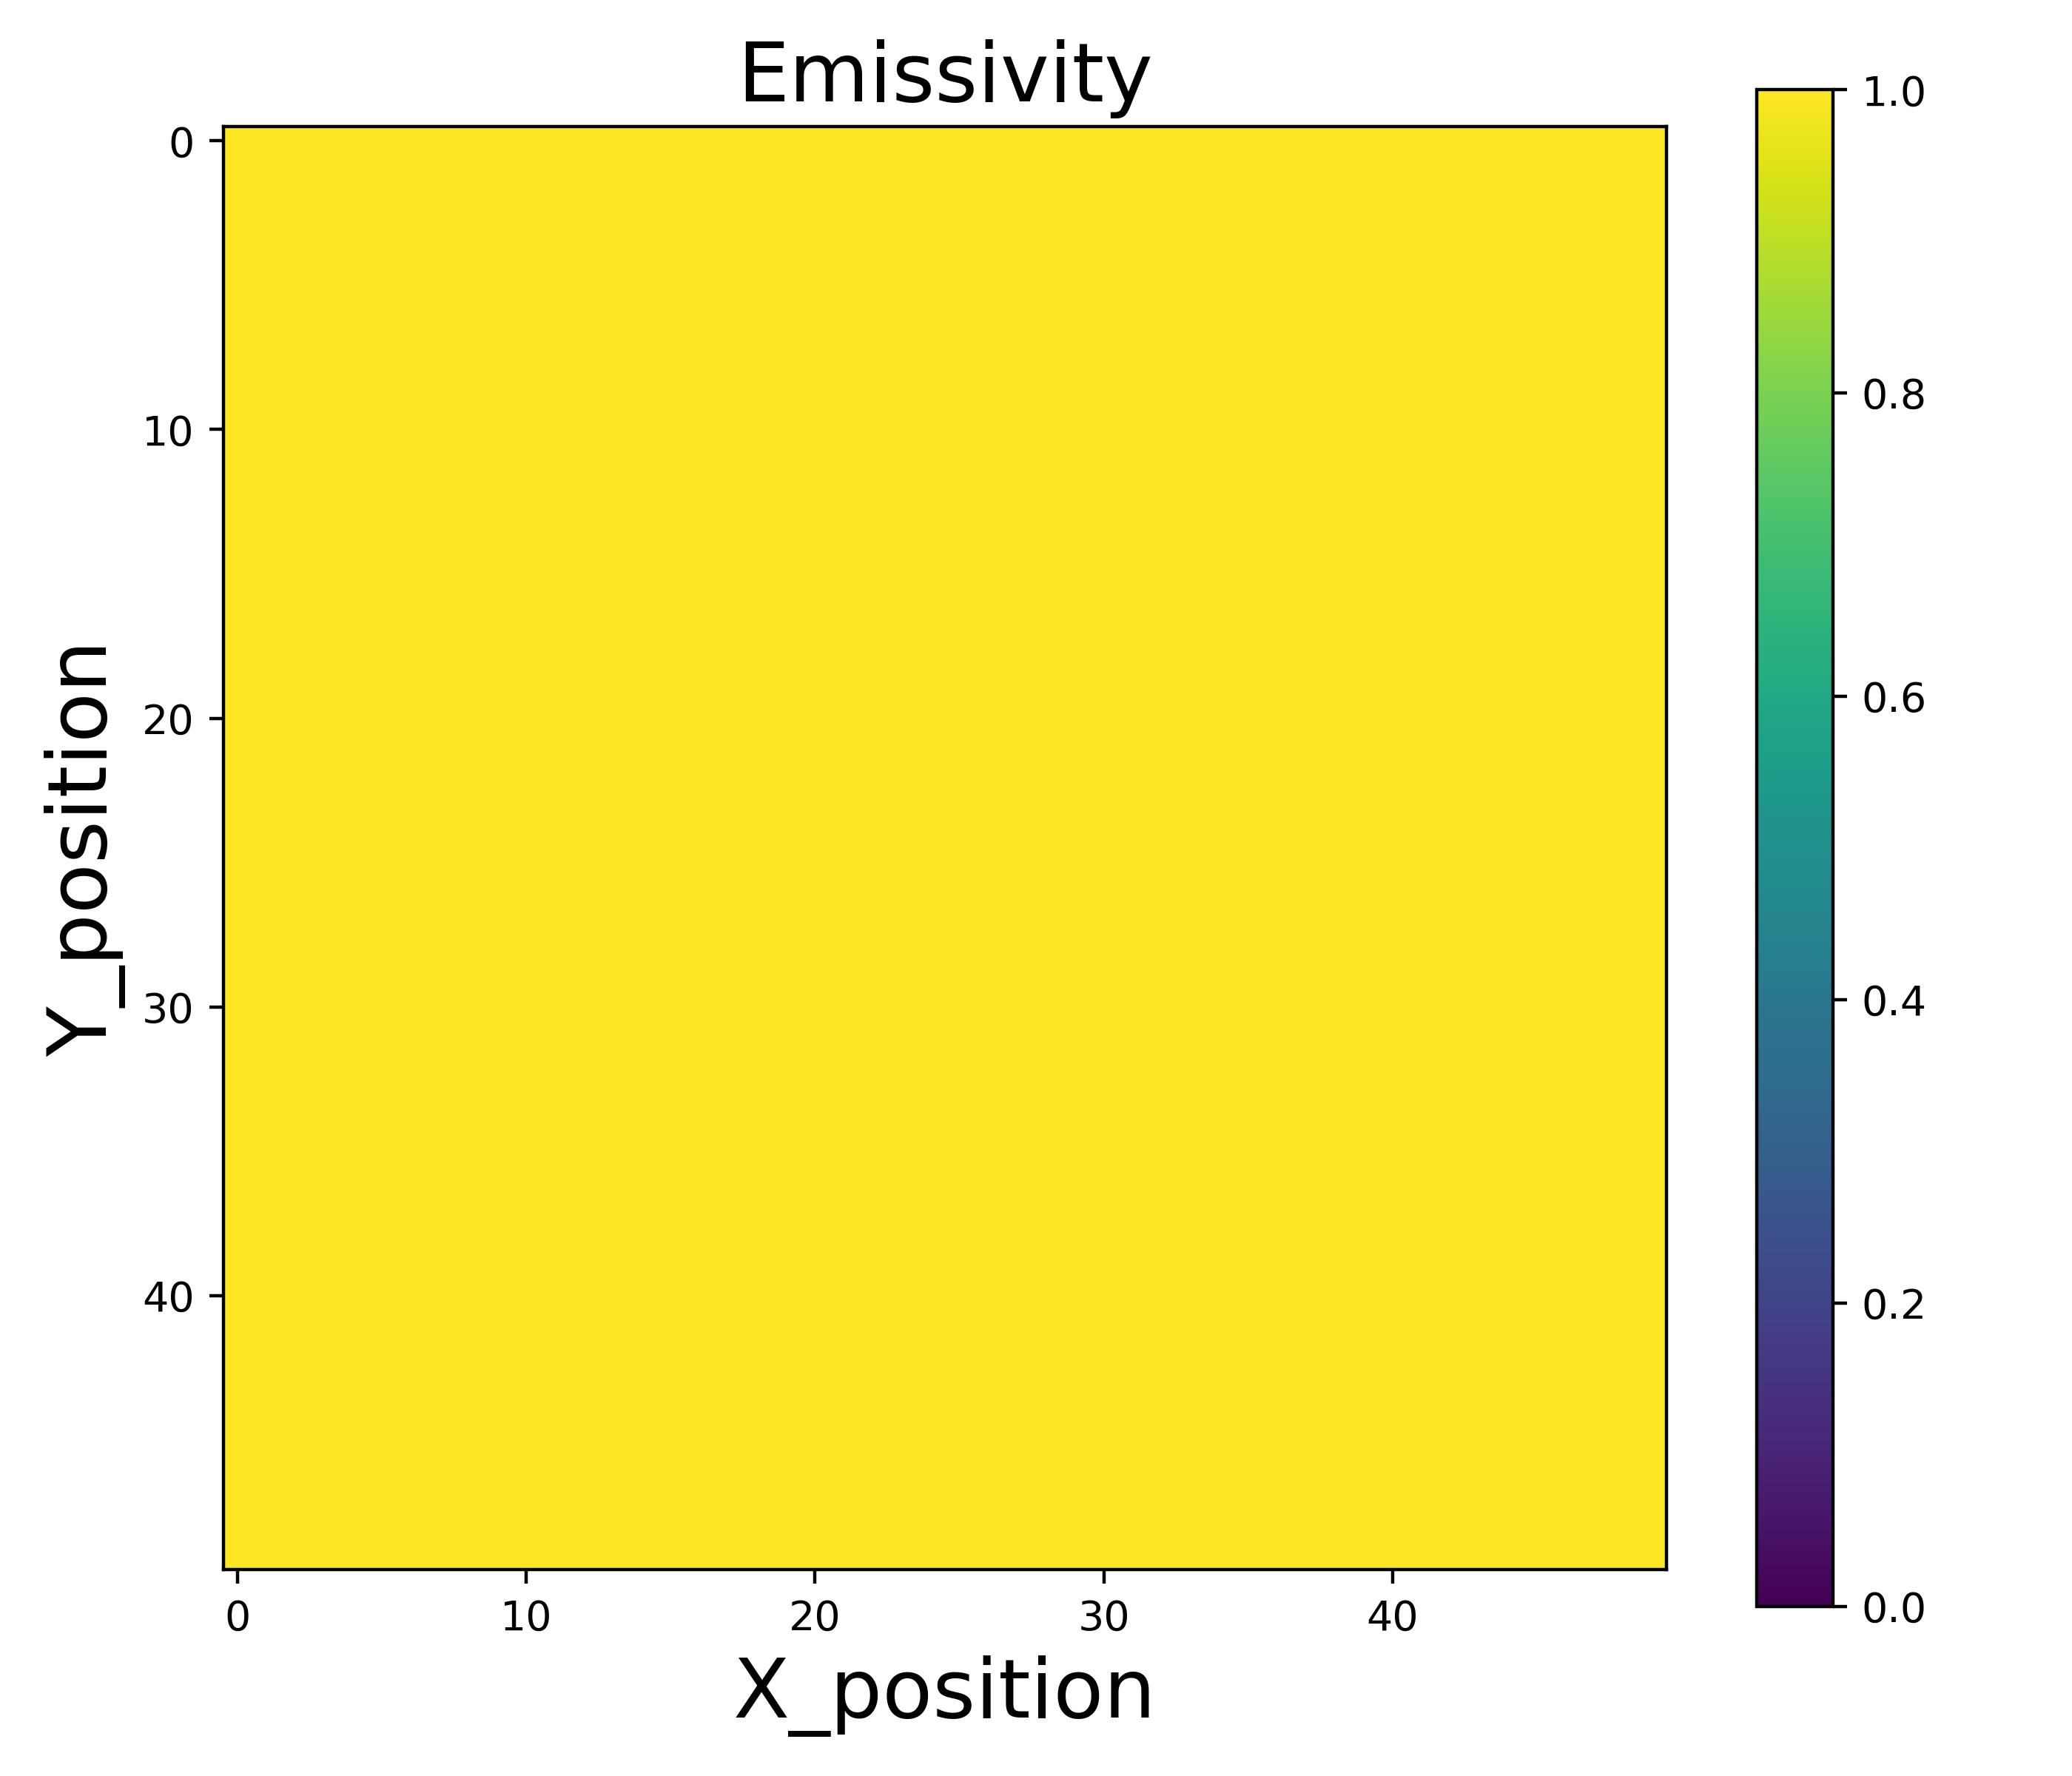
\includegraphics[width=\textwidth]{figures/raw_data/5/linear/emi_cal.jpg}
            \subcaption{Real iron data}
        \end{subfigure}
        \begin{subfigure}{0.325\textwidth}
            \centering
            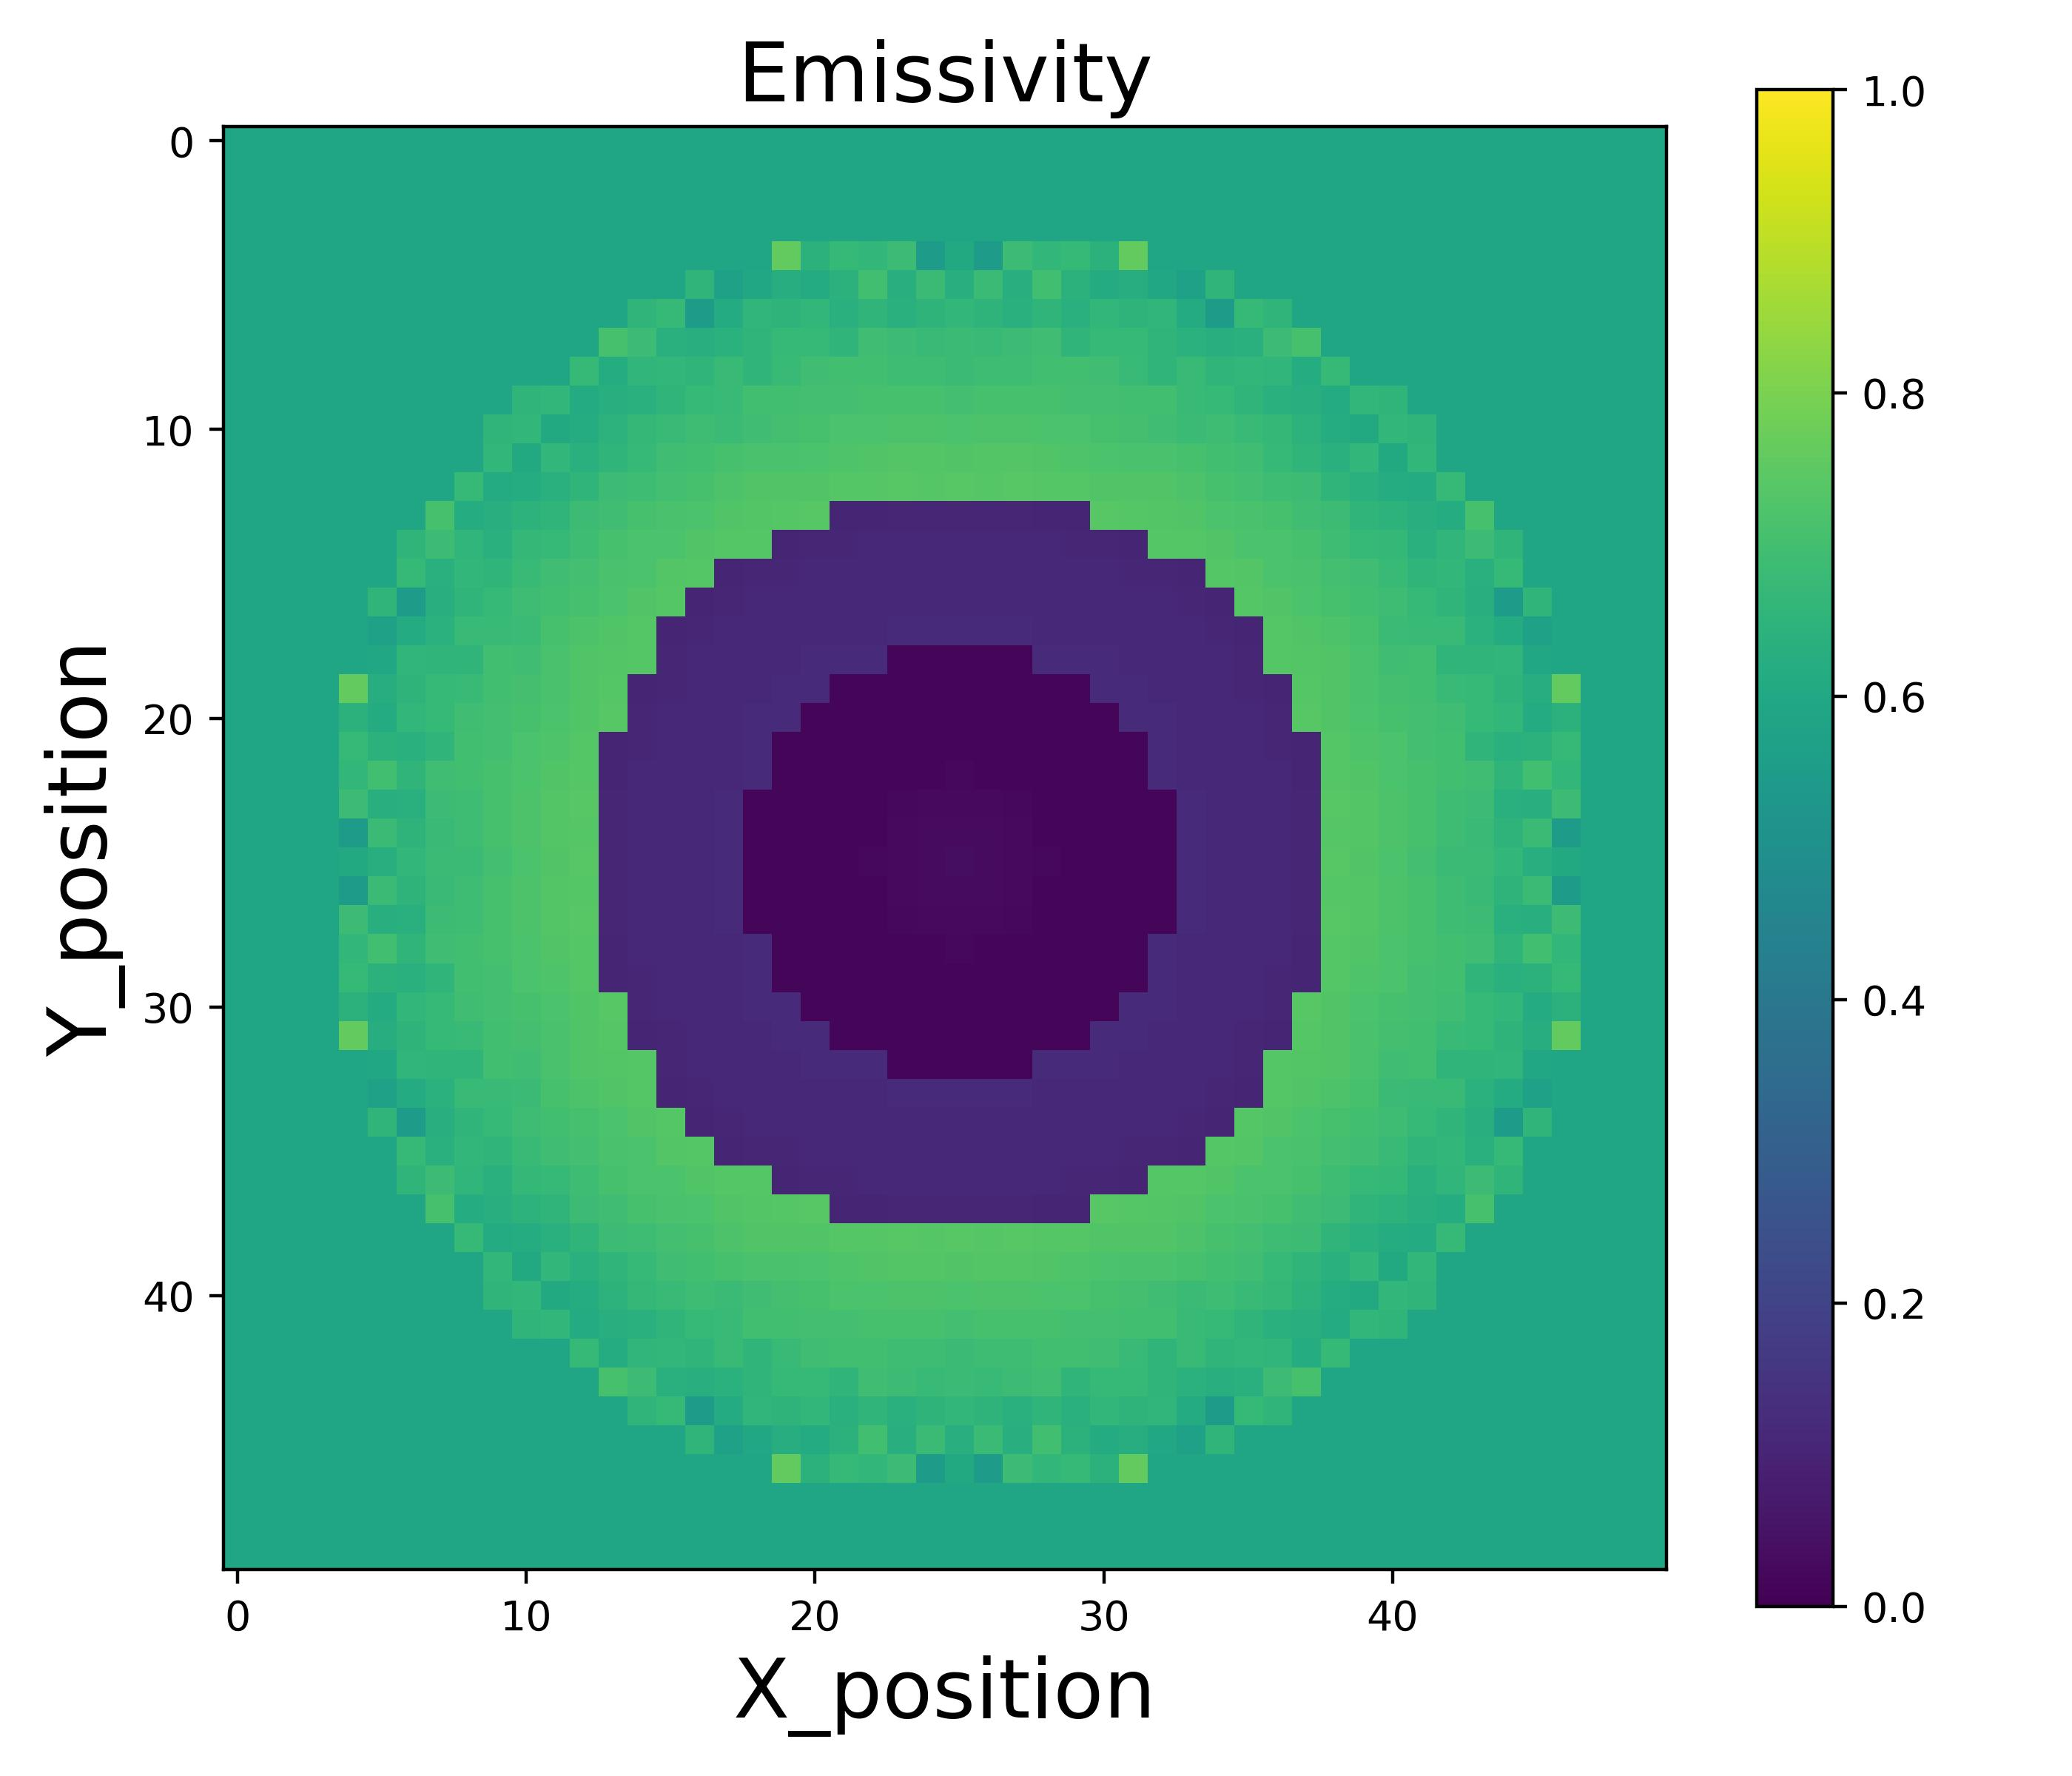
\includegraphics[width=\textwidth]{figures/raw_data/21/linear/emi_cal.jpg}
            \subcaption{Model 1}
        \end{subfigure}
    \end{minipage}\\
    \begin{minipage}{\textwidth}
        \centering
        \begin{subfigure}{0.325\textwidth}
            \centering
            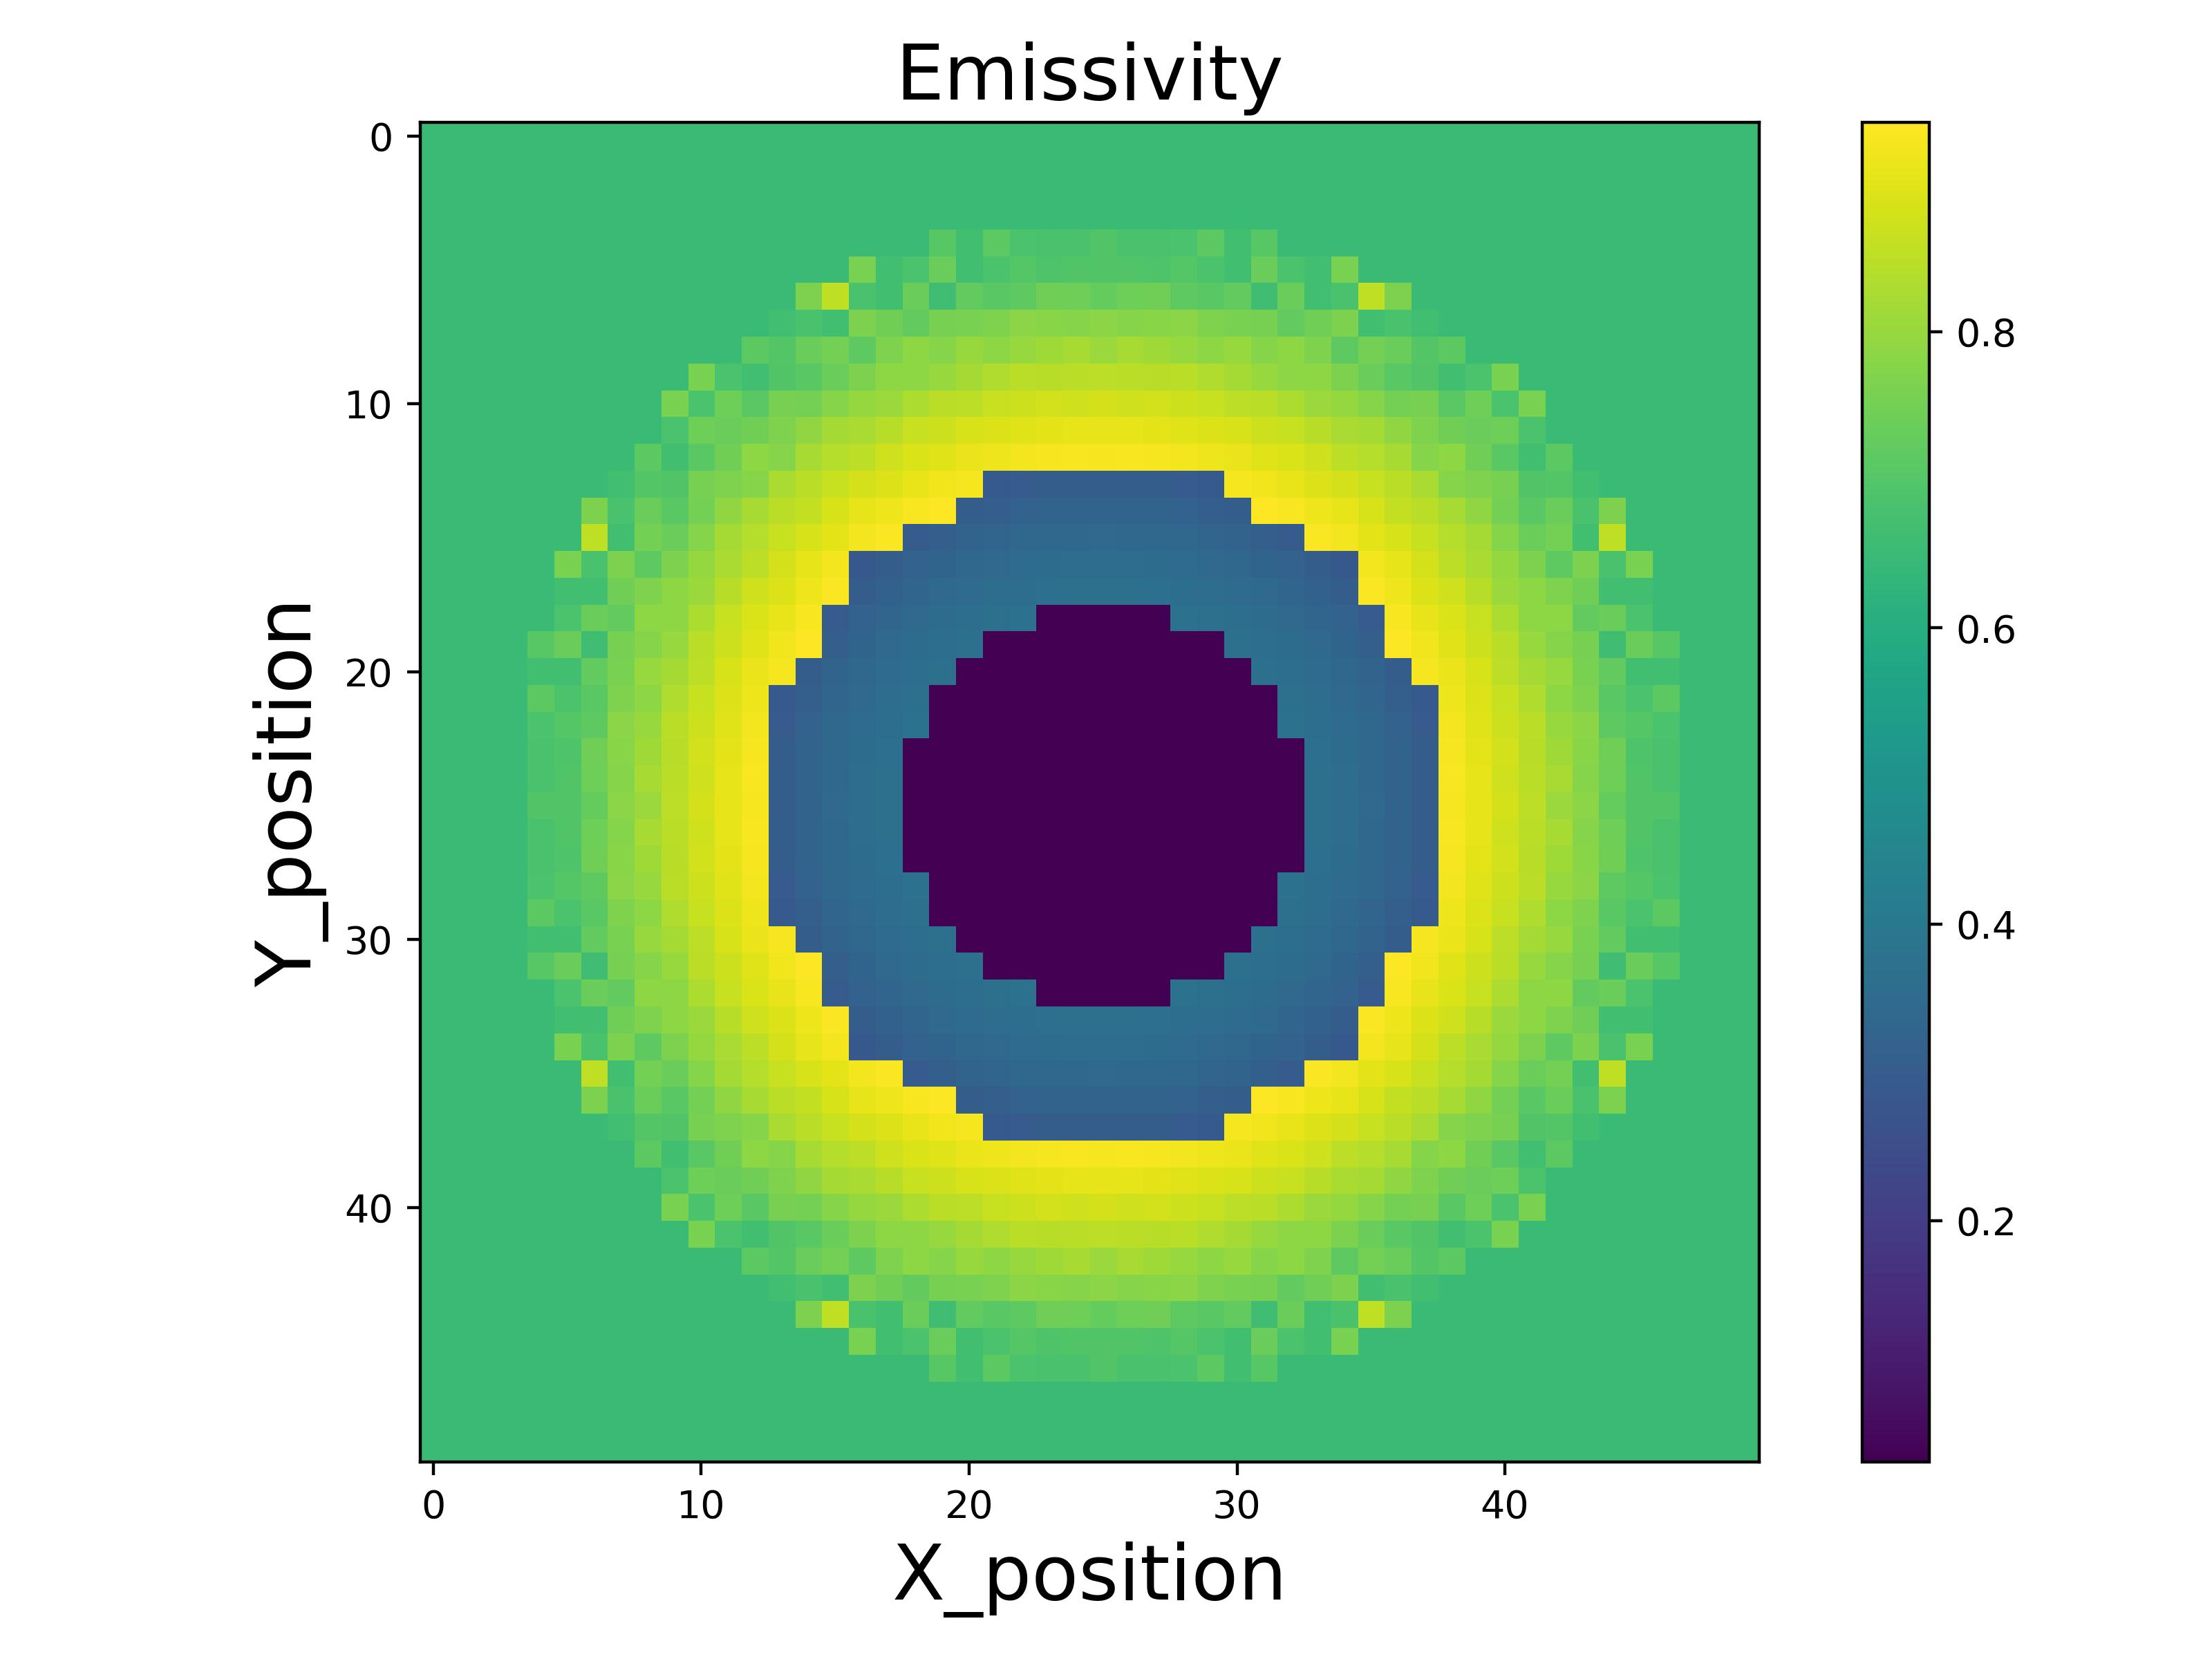
\includegraphics[width=\textwidth]{figures/raw_data/22/linear/emi_cal.jpg}
            \subcaption{Model 2}
        \end{subfigure}
        \begin{subfigure}{0.325\textwidth}
            \centering
            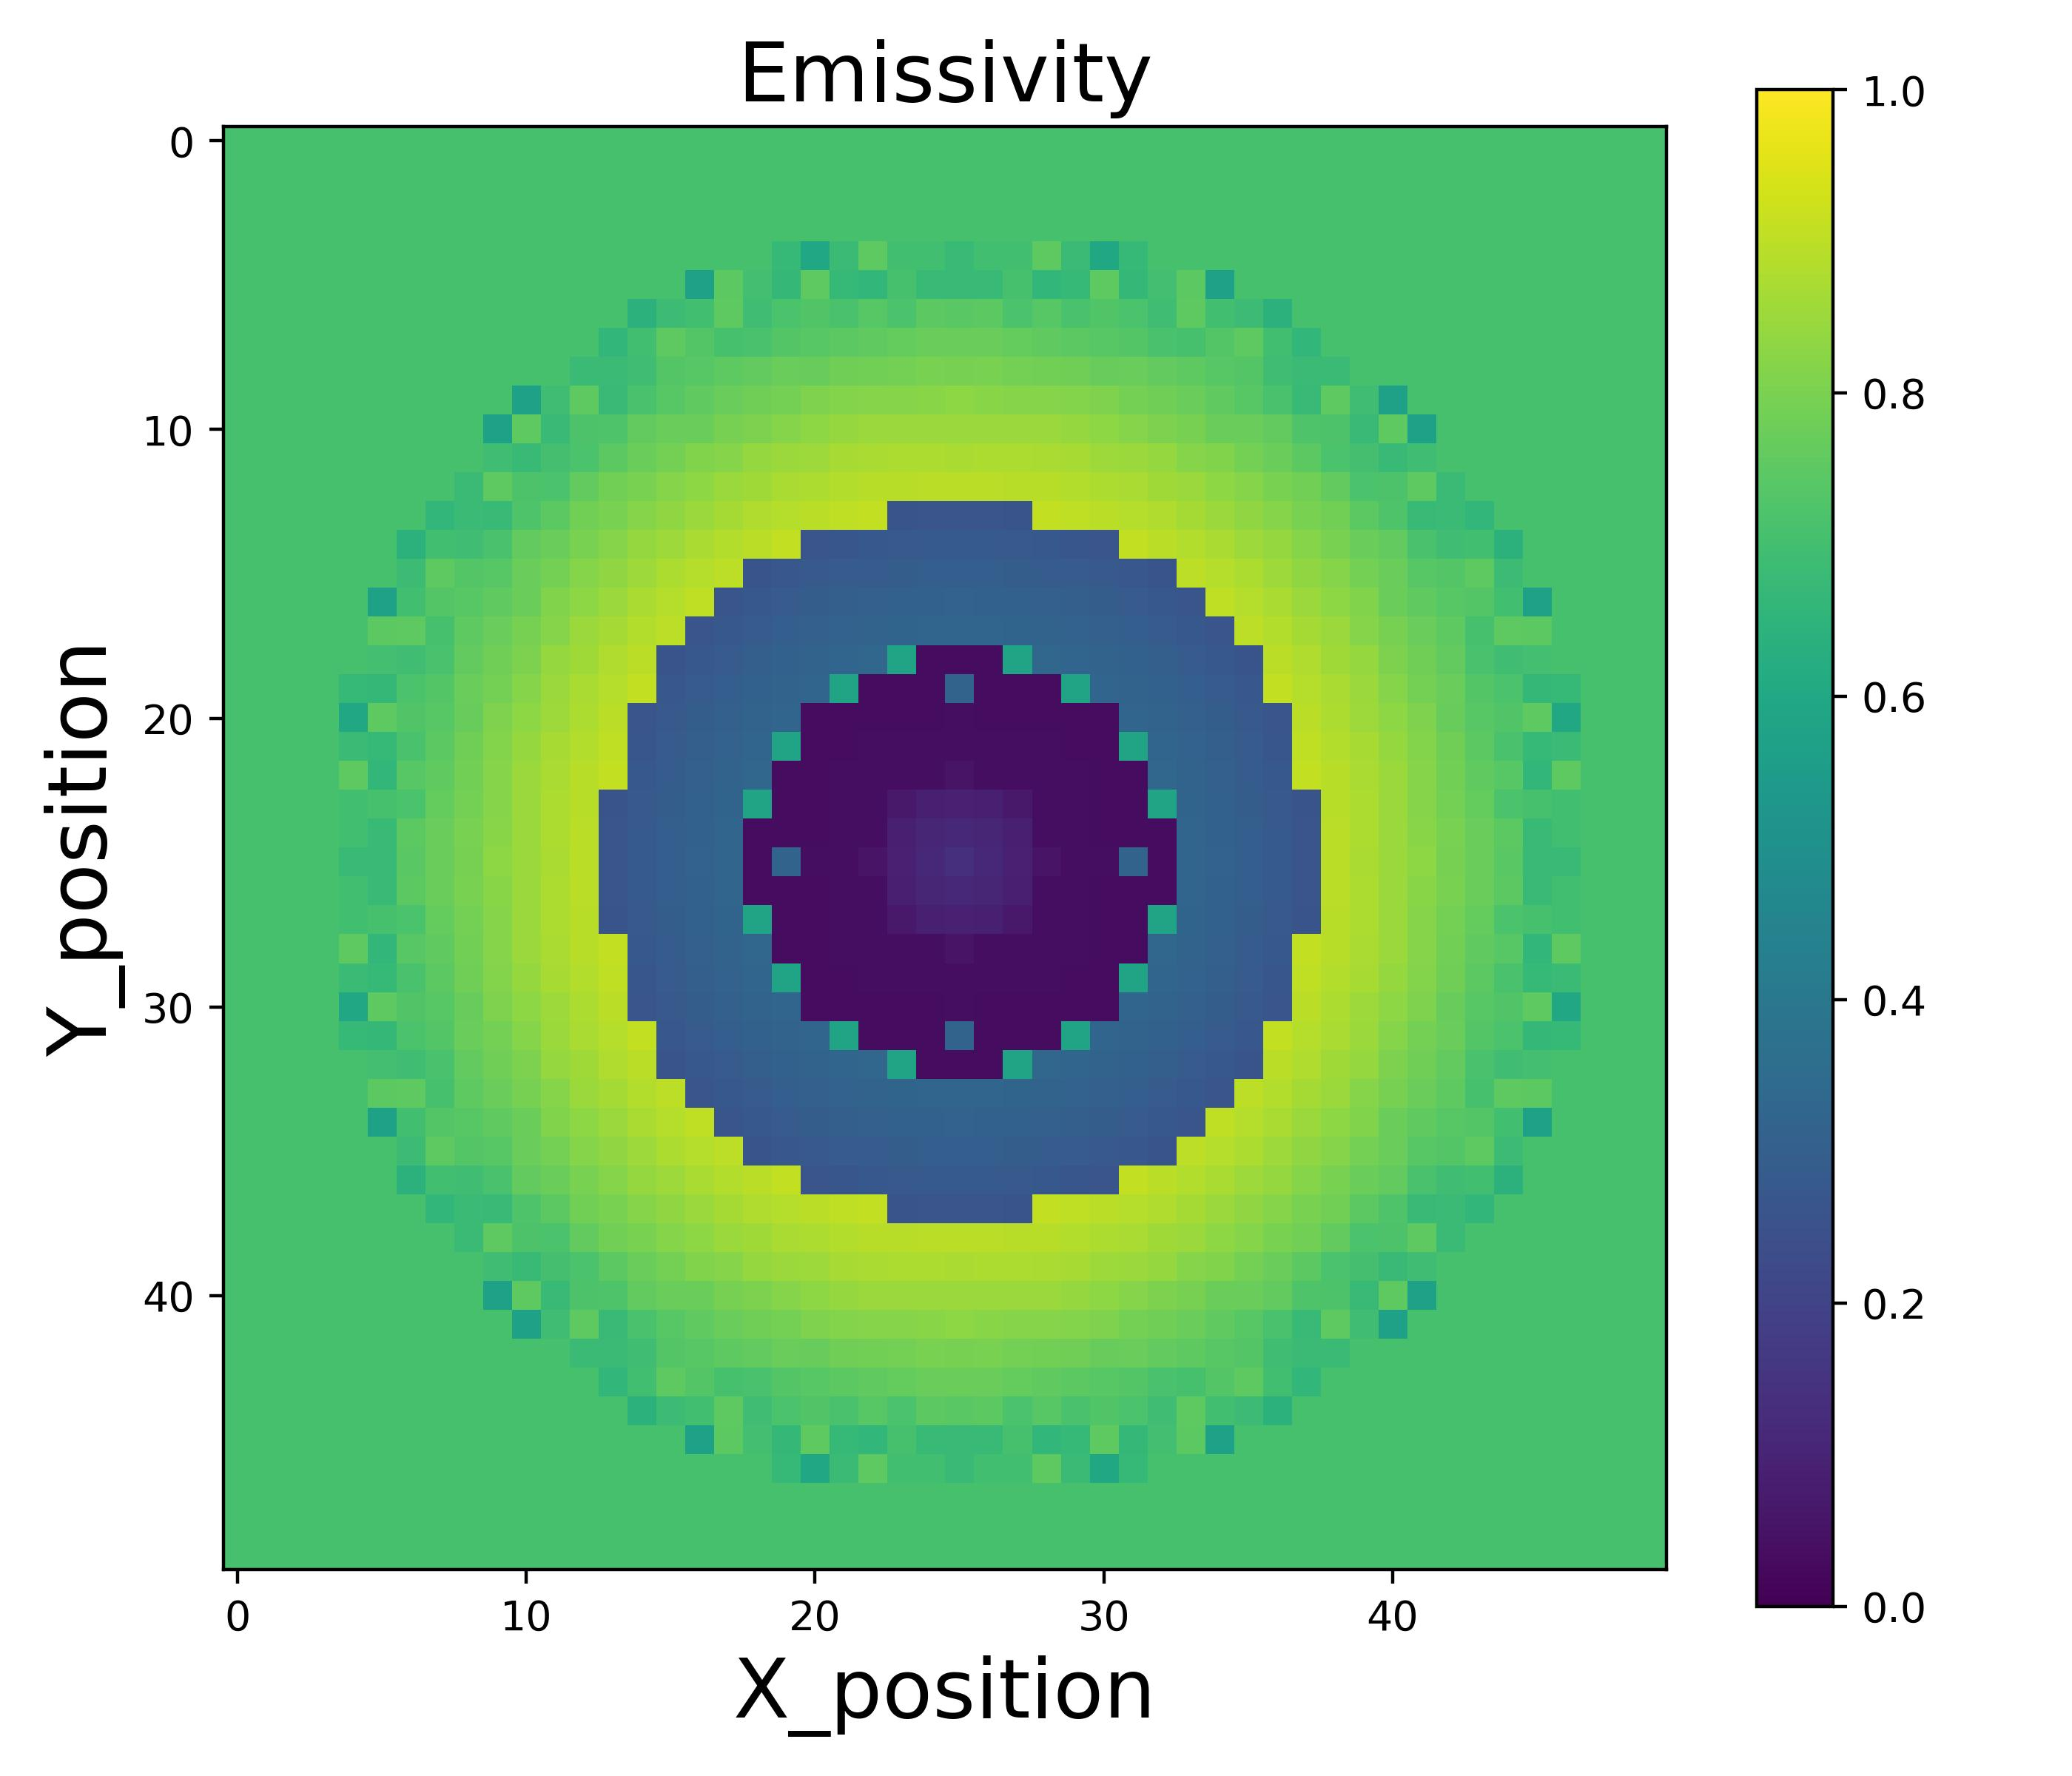
\includegraphics[width=\textwidth]{figures/raw_data/23/linear/emi_cal.jpg}
            \subcaption{Model 3}
        \end{subfigure}
        \begin{subfigure}{0.325\textwidth}
            \centering
            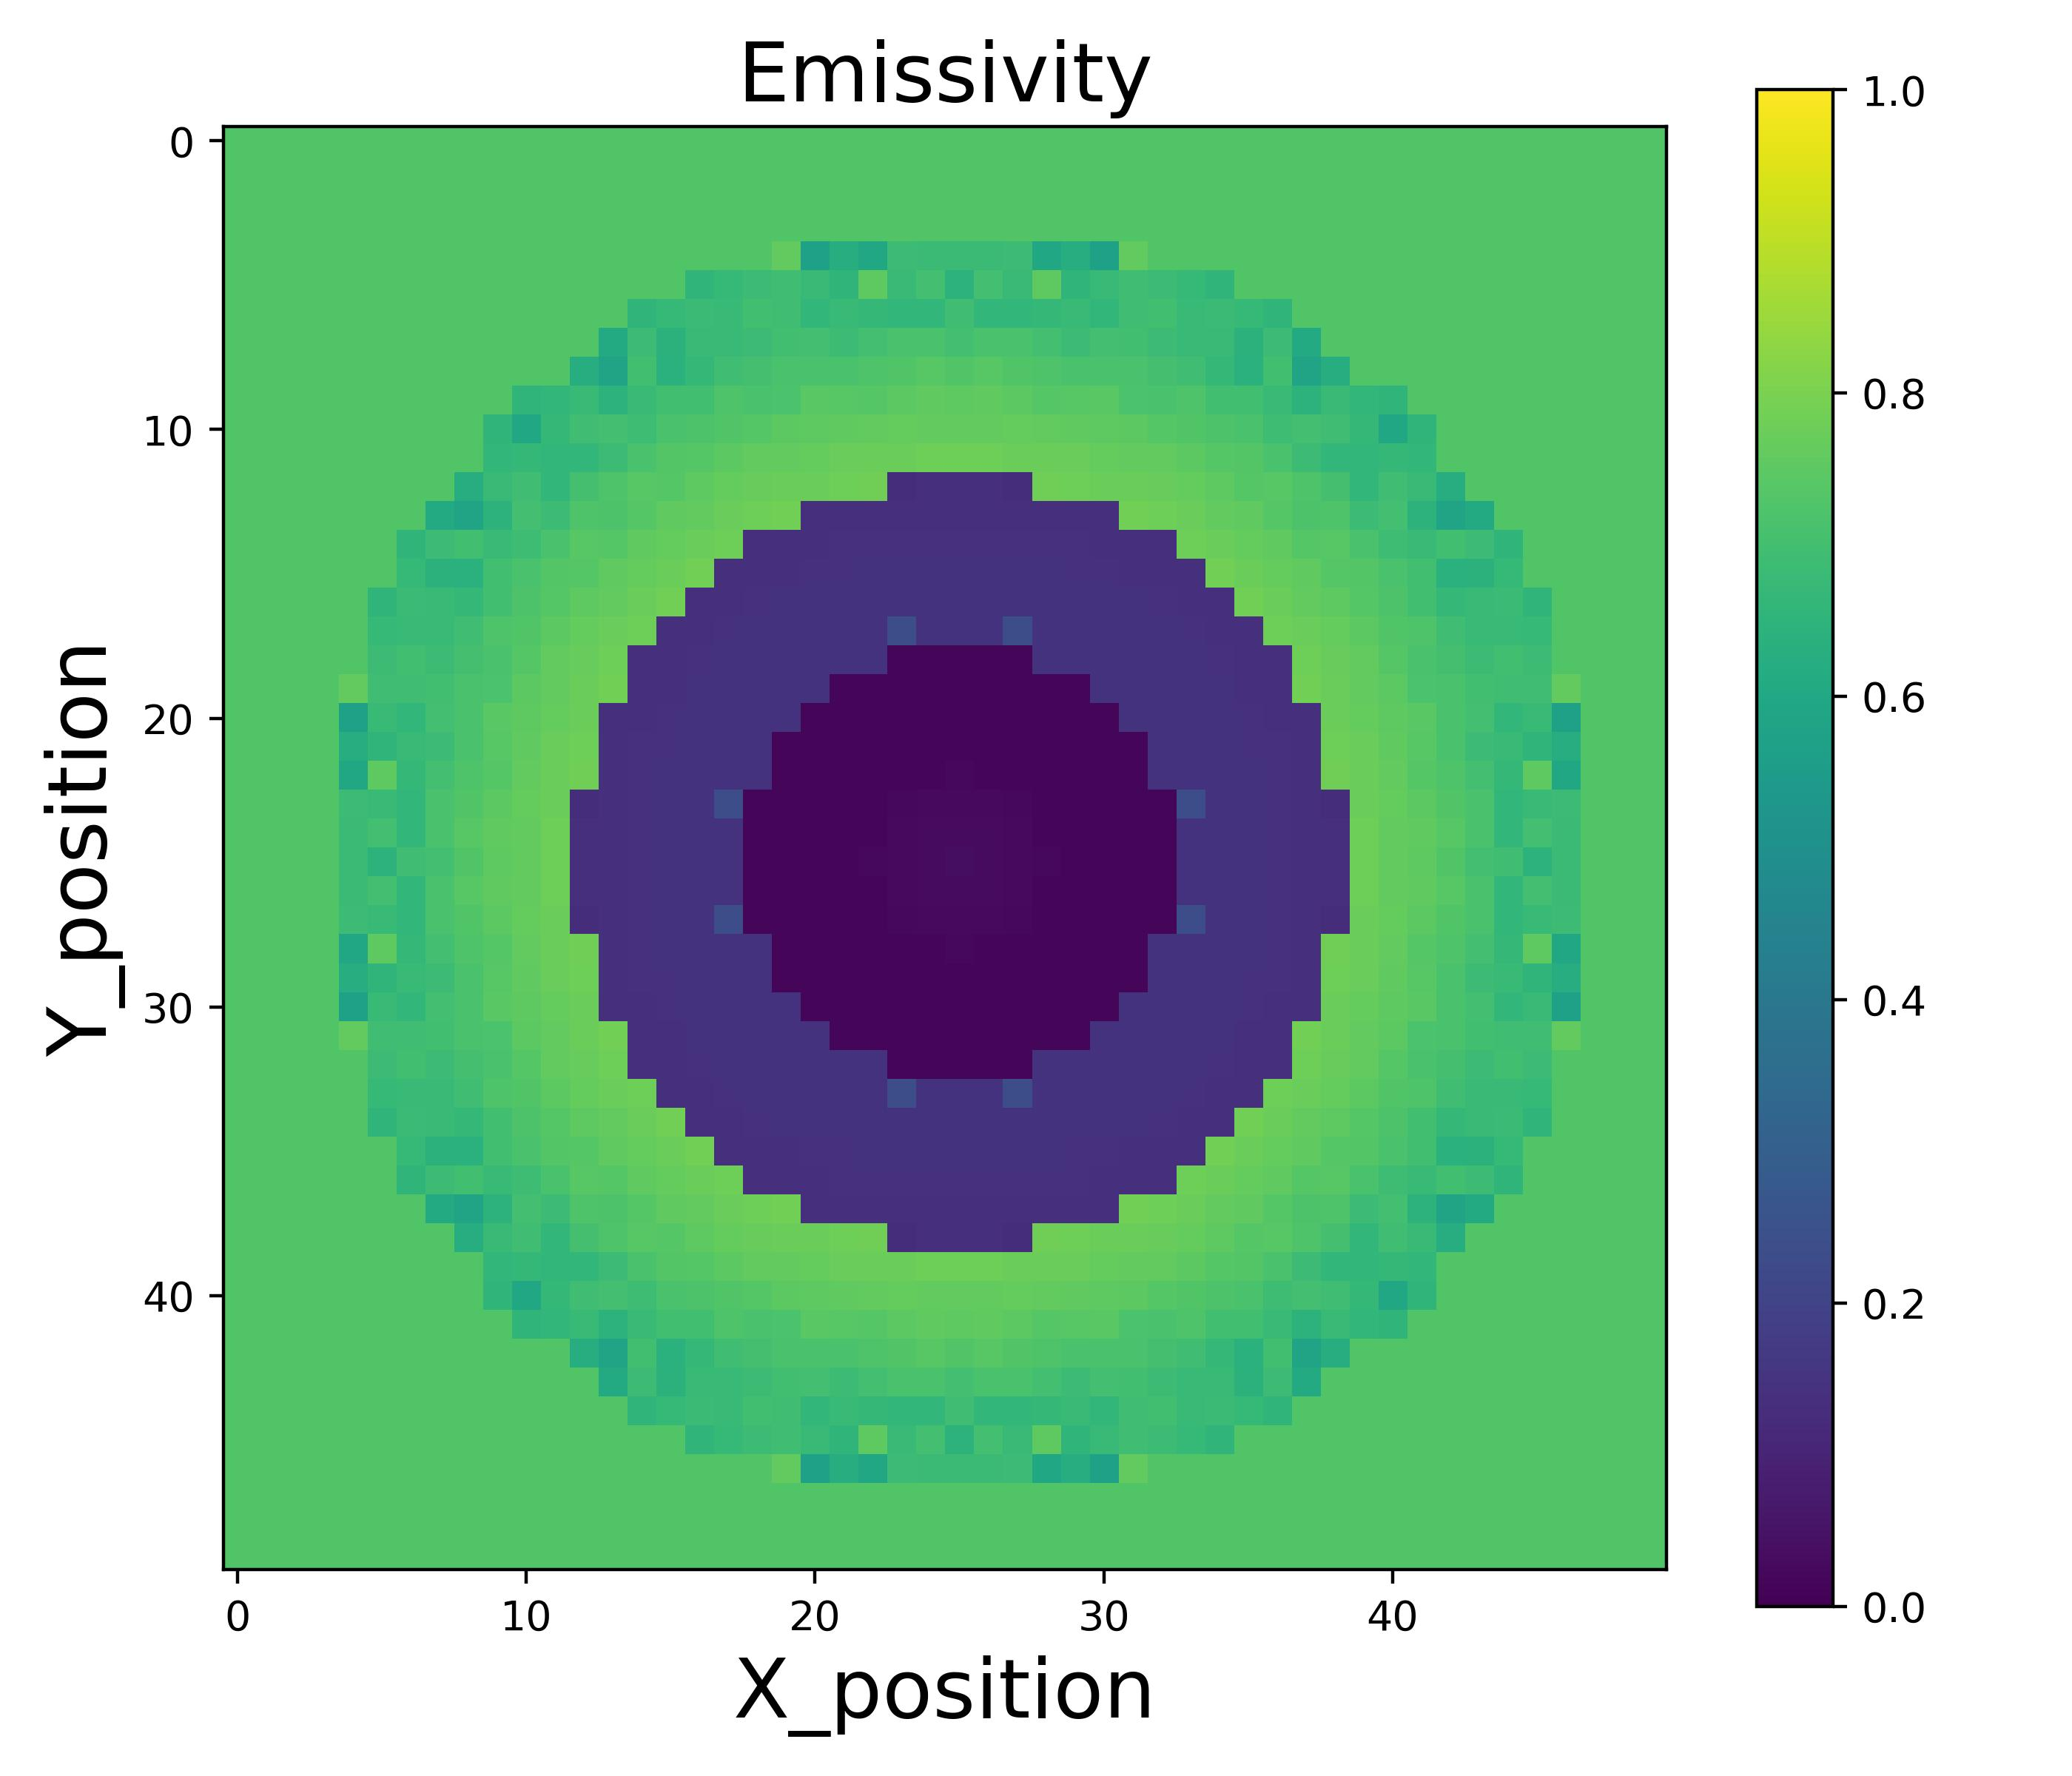
\includegraphics[width=\textwidth]{figures/raw_data/24/linear/emi_cal.jpg}
            \subcaption{Model 4}
        \end{subfigure}
    \end{minipage}\\
    \begin{minipage}{\textwidth}
        \centering
        \begin{subfigure}{0.325\textwidth}
            \centering
            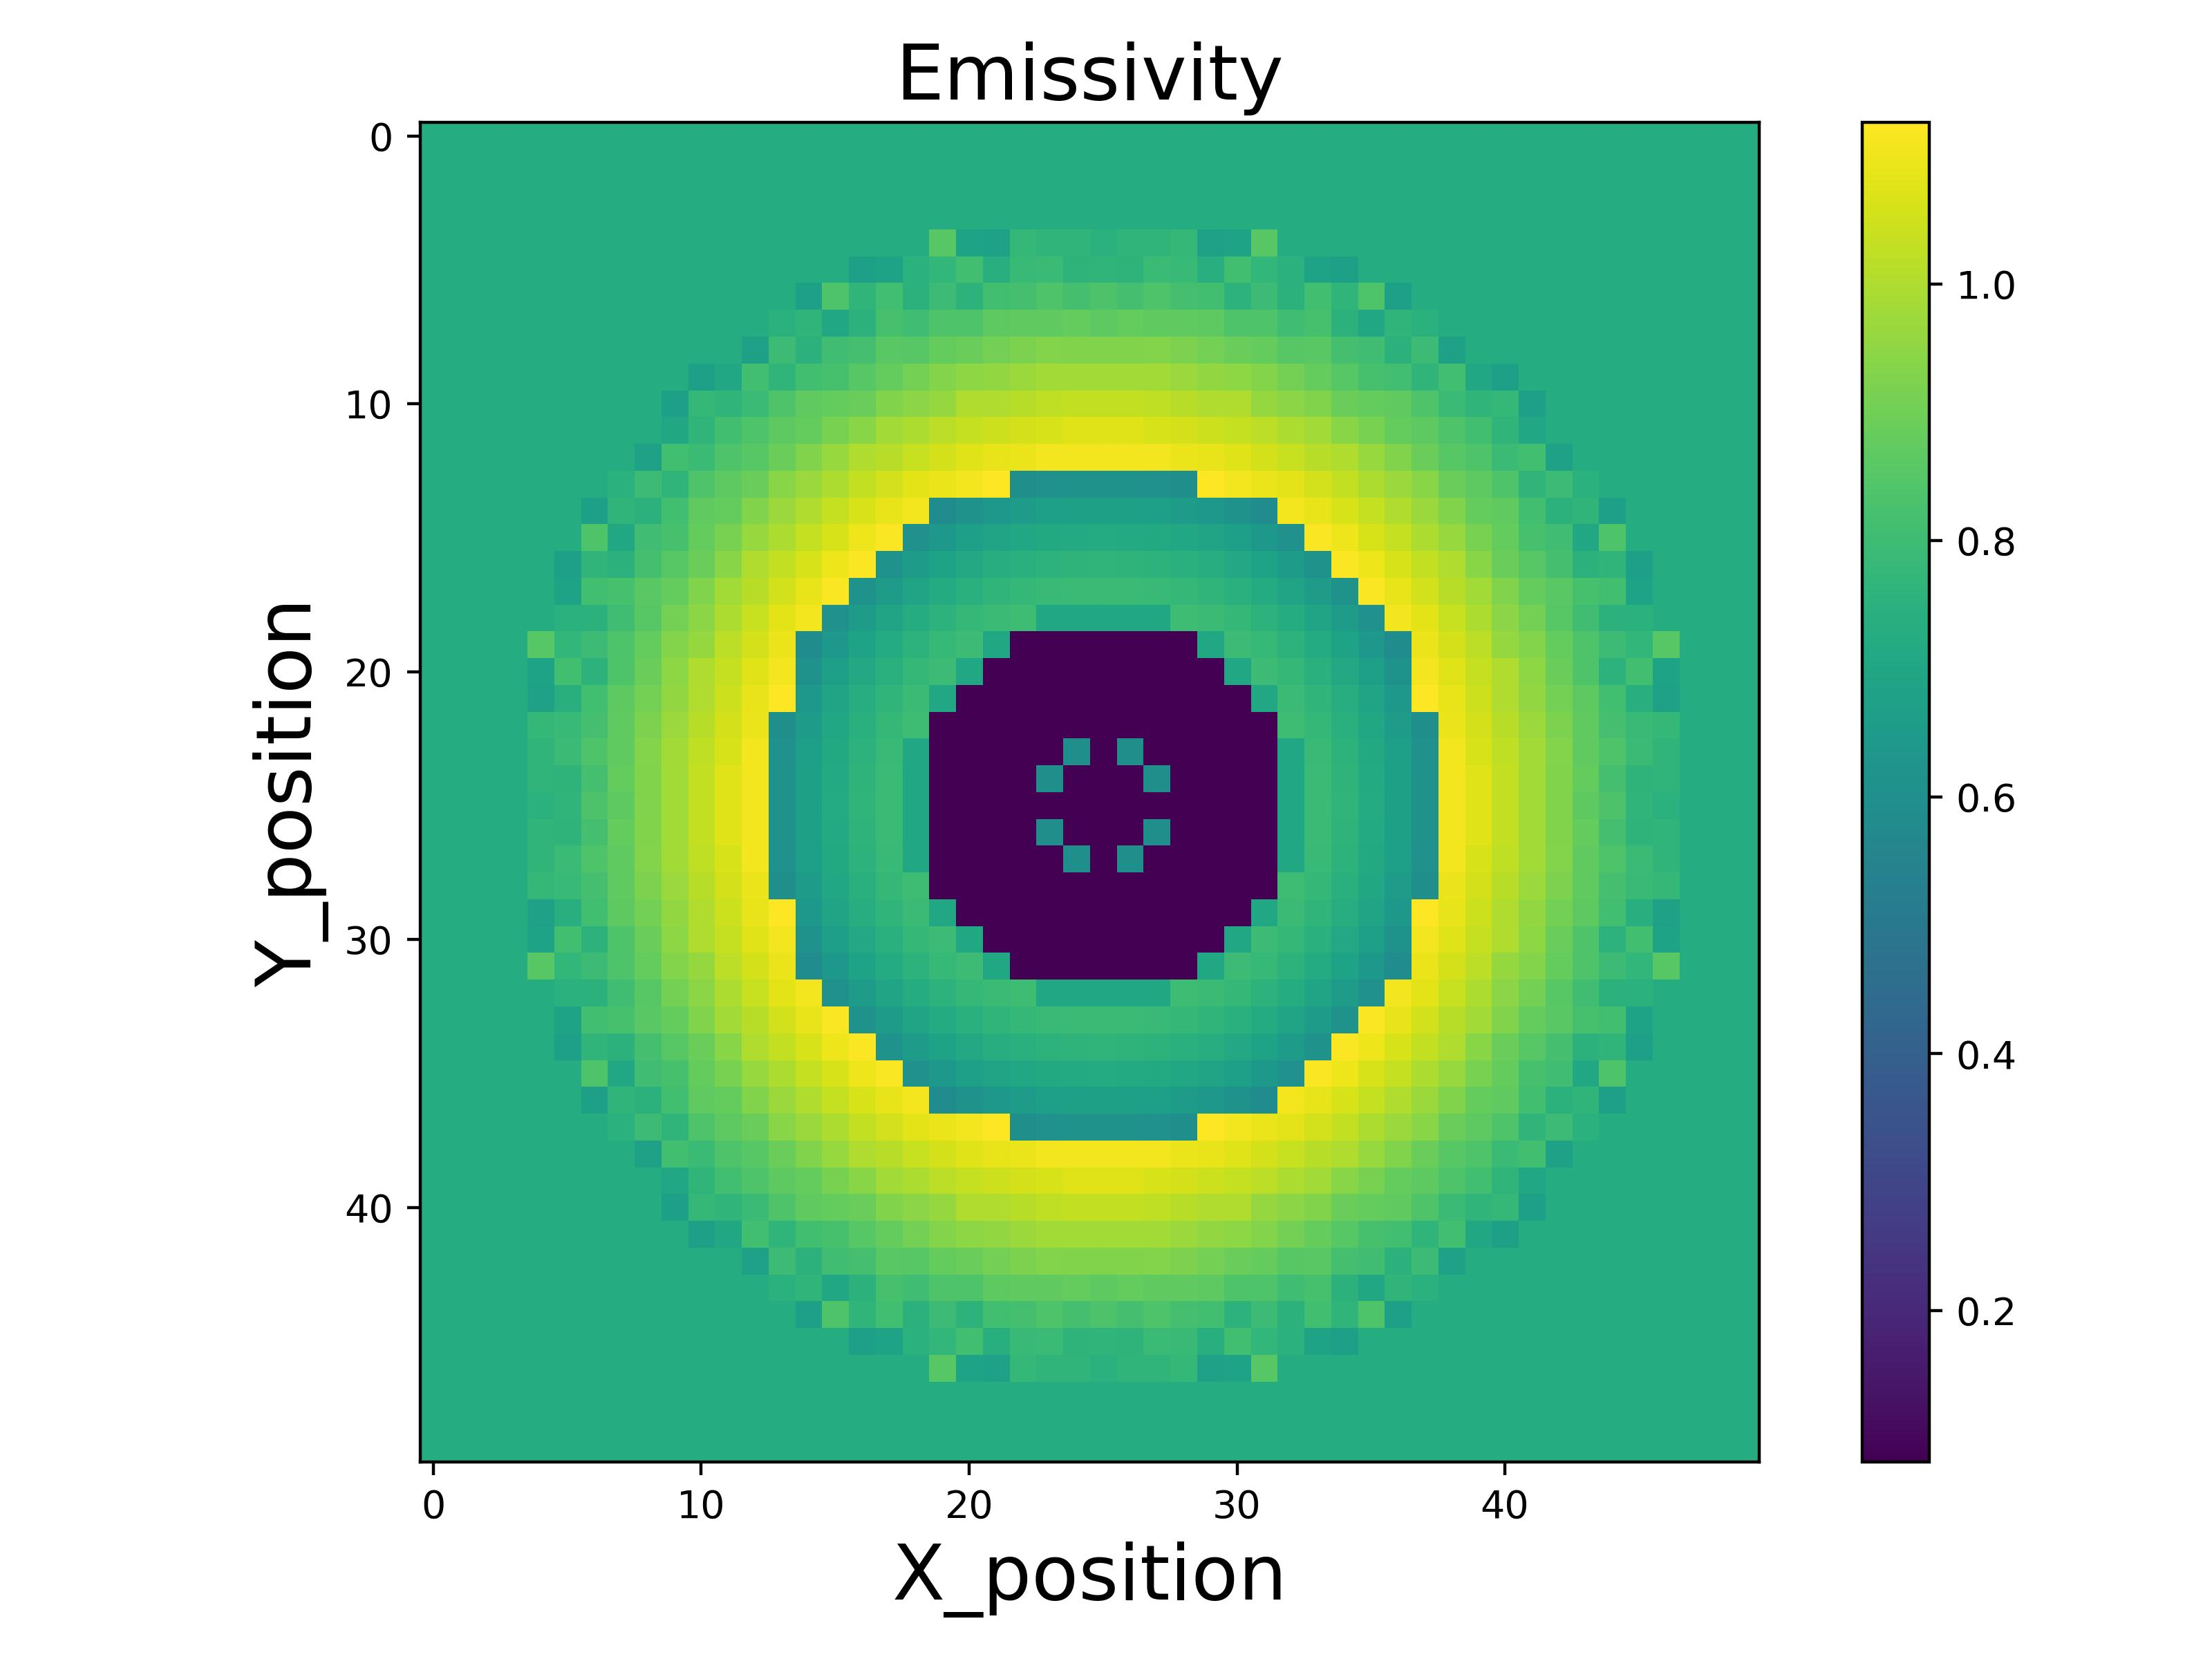
\includegraphics[width=\textwidth]{figures/raw_data/25/linear/emi_cal.jpg}
            \subcaption{Model 5}
        \end{subfigure}
        \begin{subfigure}{0.325\textwidth}
            \centering
            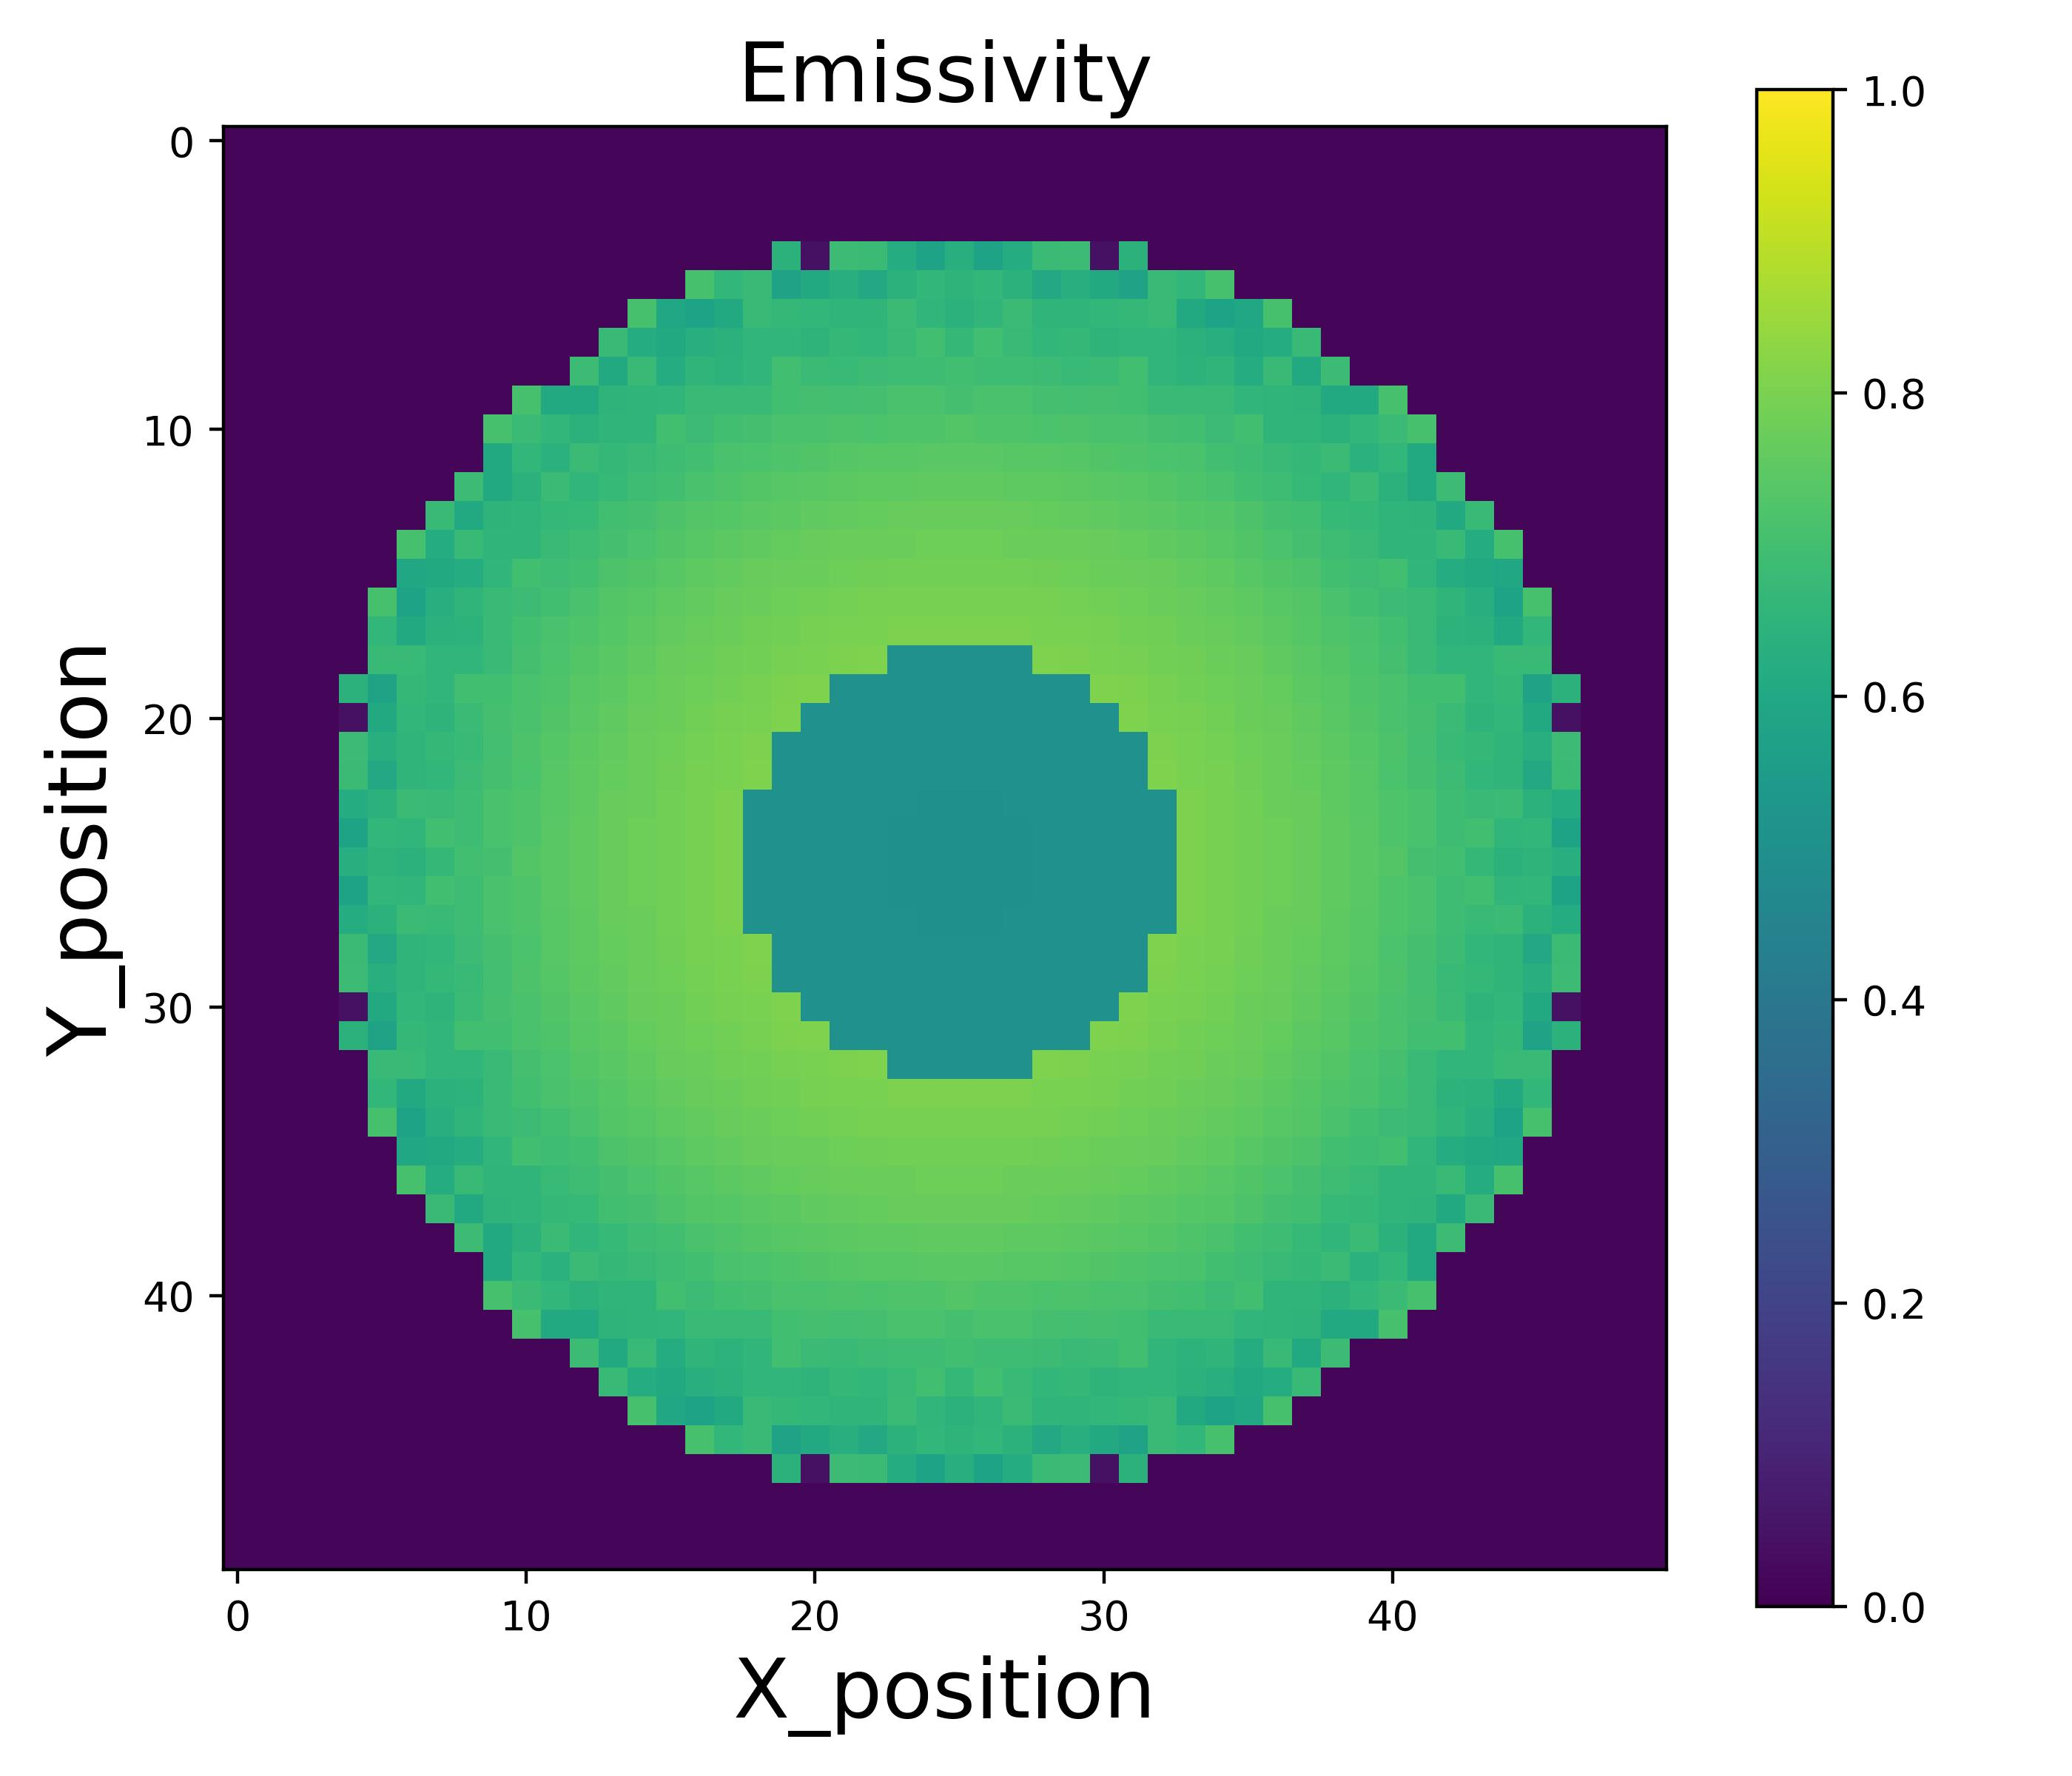
\includegraphics[width=\textwidth]{figures/raw_data/26/linear/emi_cal.jpg}
            \subcaption{Model 6}
        \end{subfigure}
        \begin{subfigure}{0.325\textwidth}
            \centering
            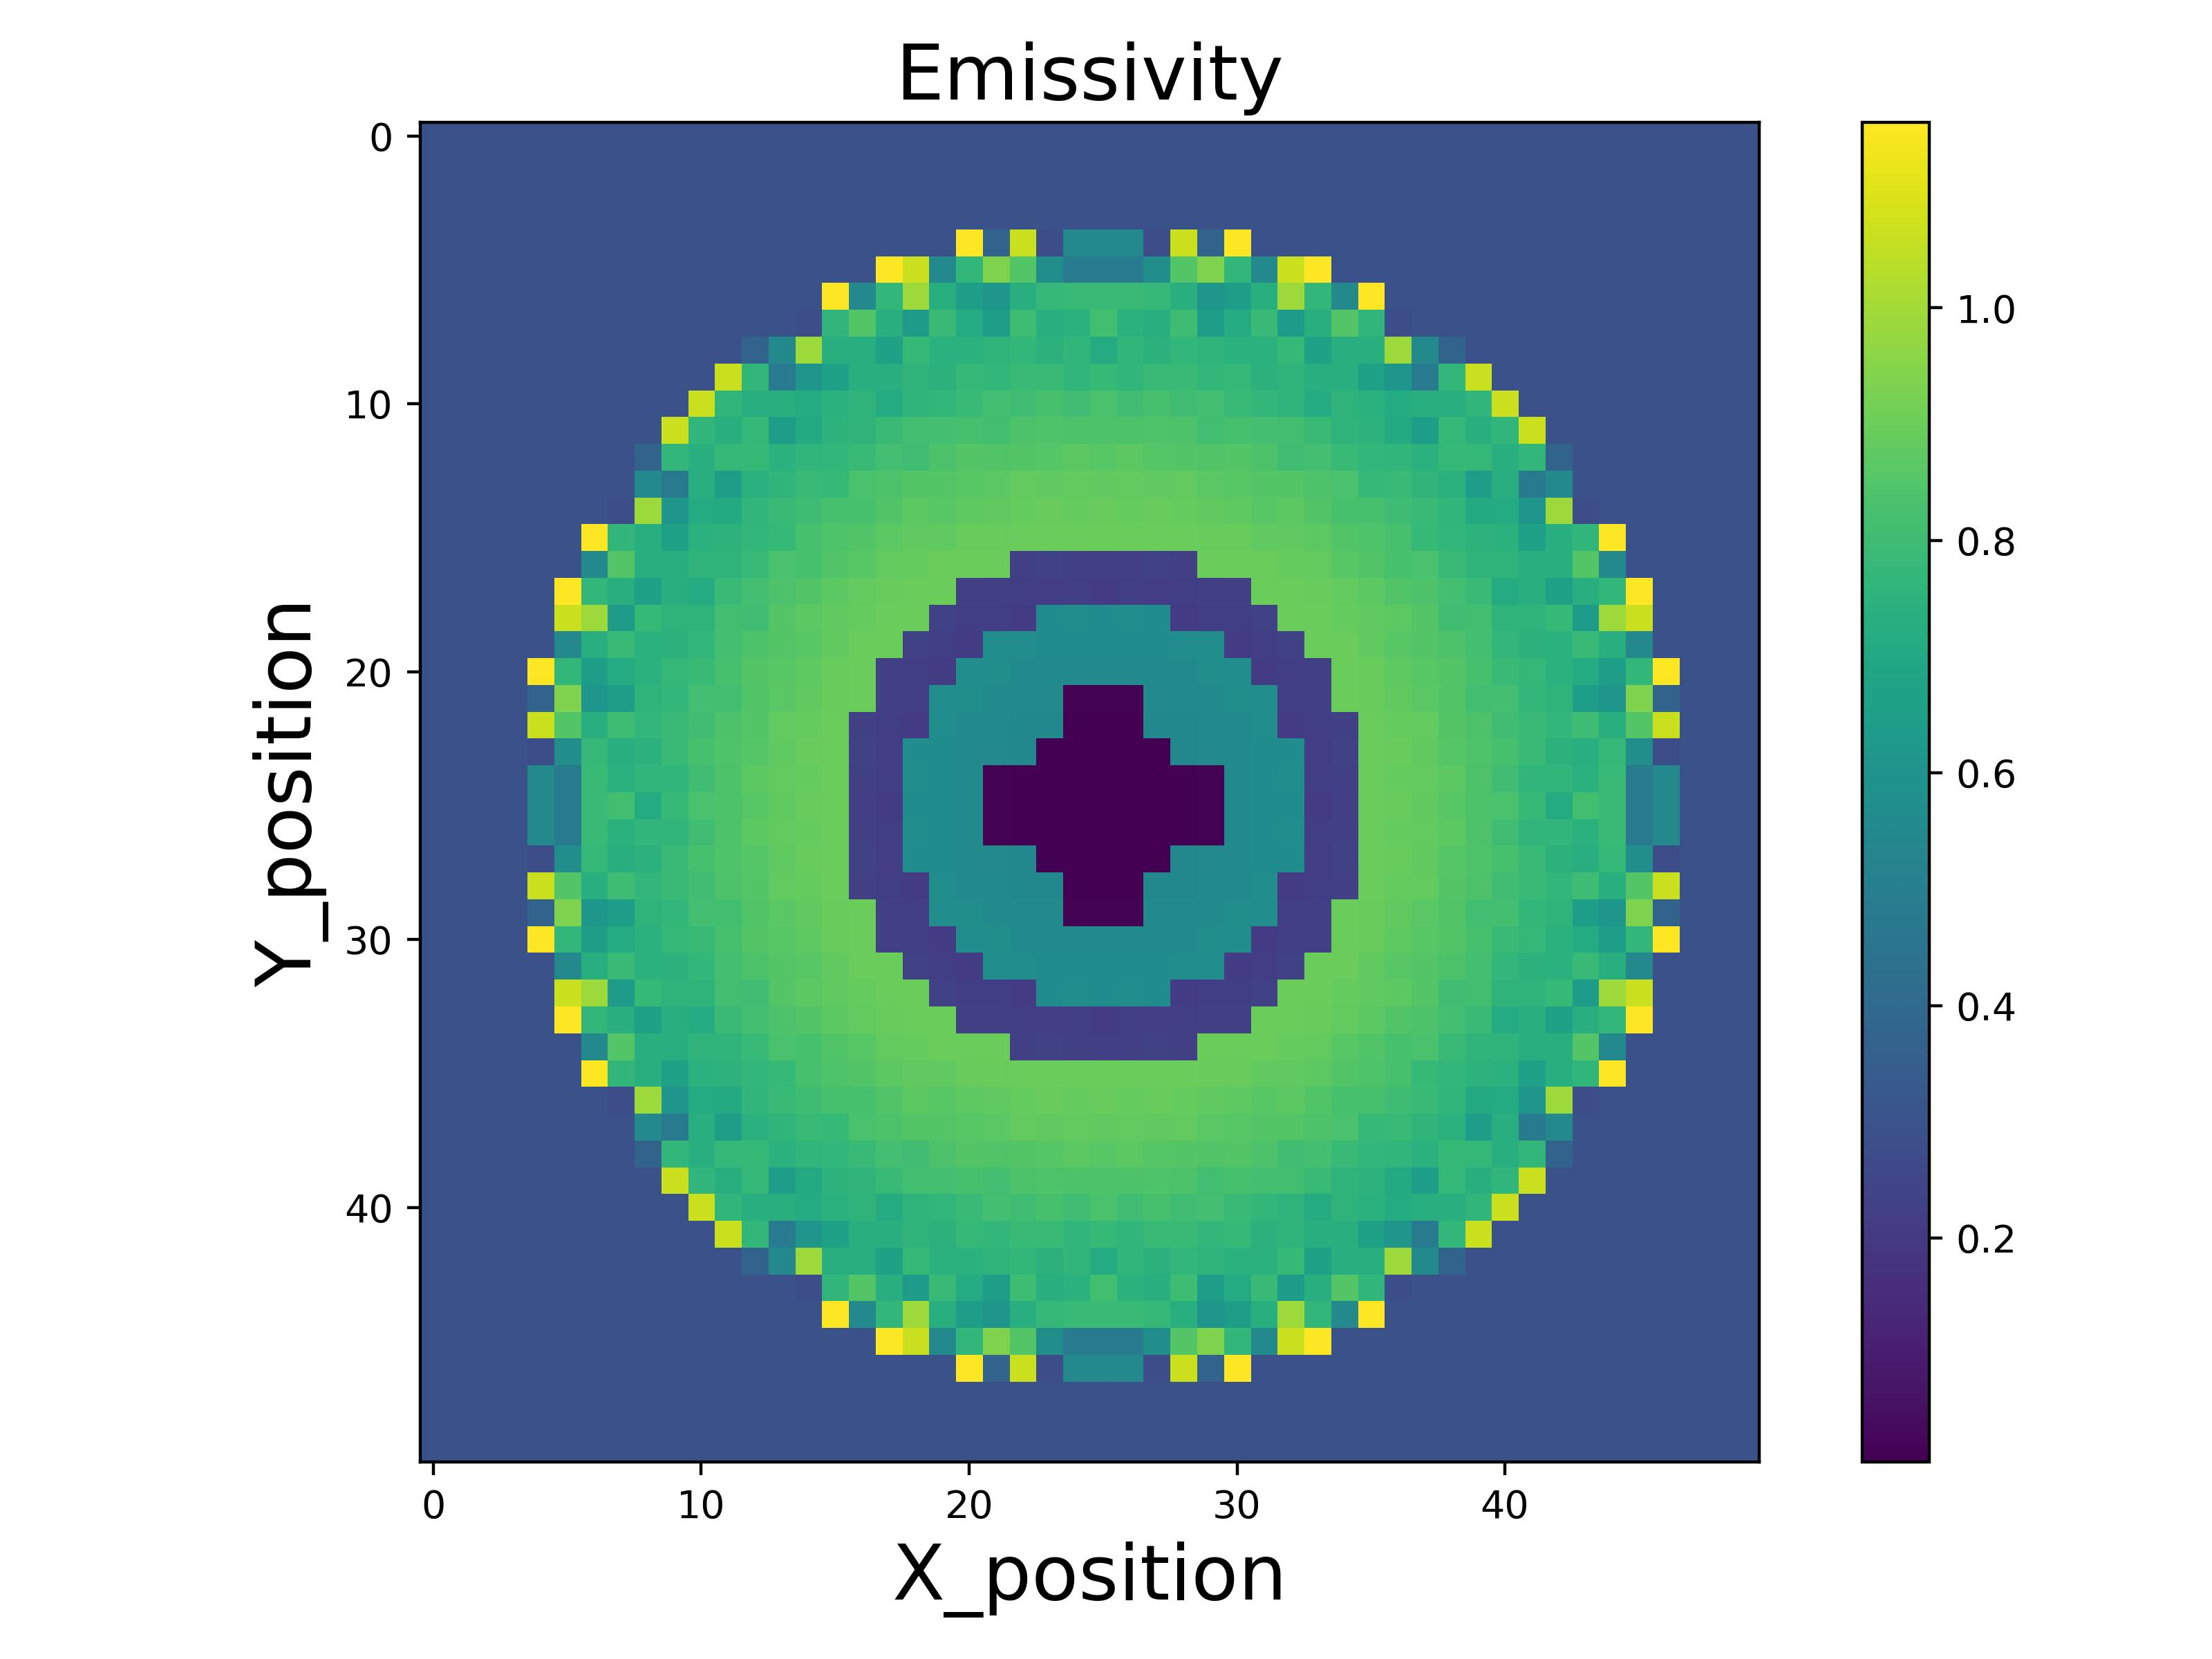
\includegraphics[width=\textwidth]{figures/raw_data/31/linear/emi_cal.jpg}
            \subcaption{Model 7}
        \end{subfigure}
    \end{minipage}\\
    \begin{minipage}{\textwidth}
        \centering
        \begin{subfigure}{0.325\textwidth}
            \centering
            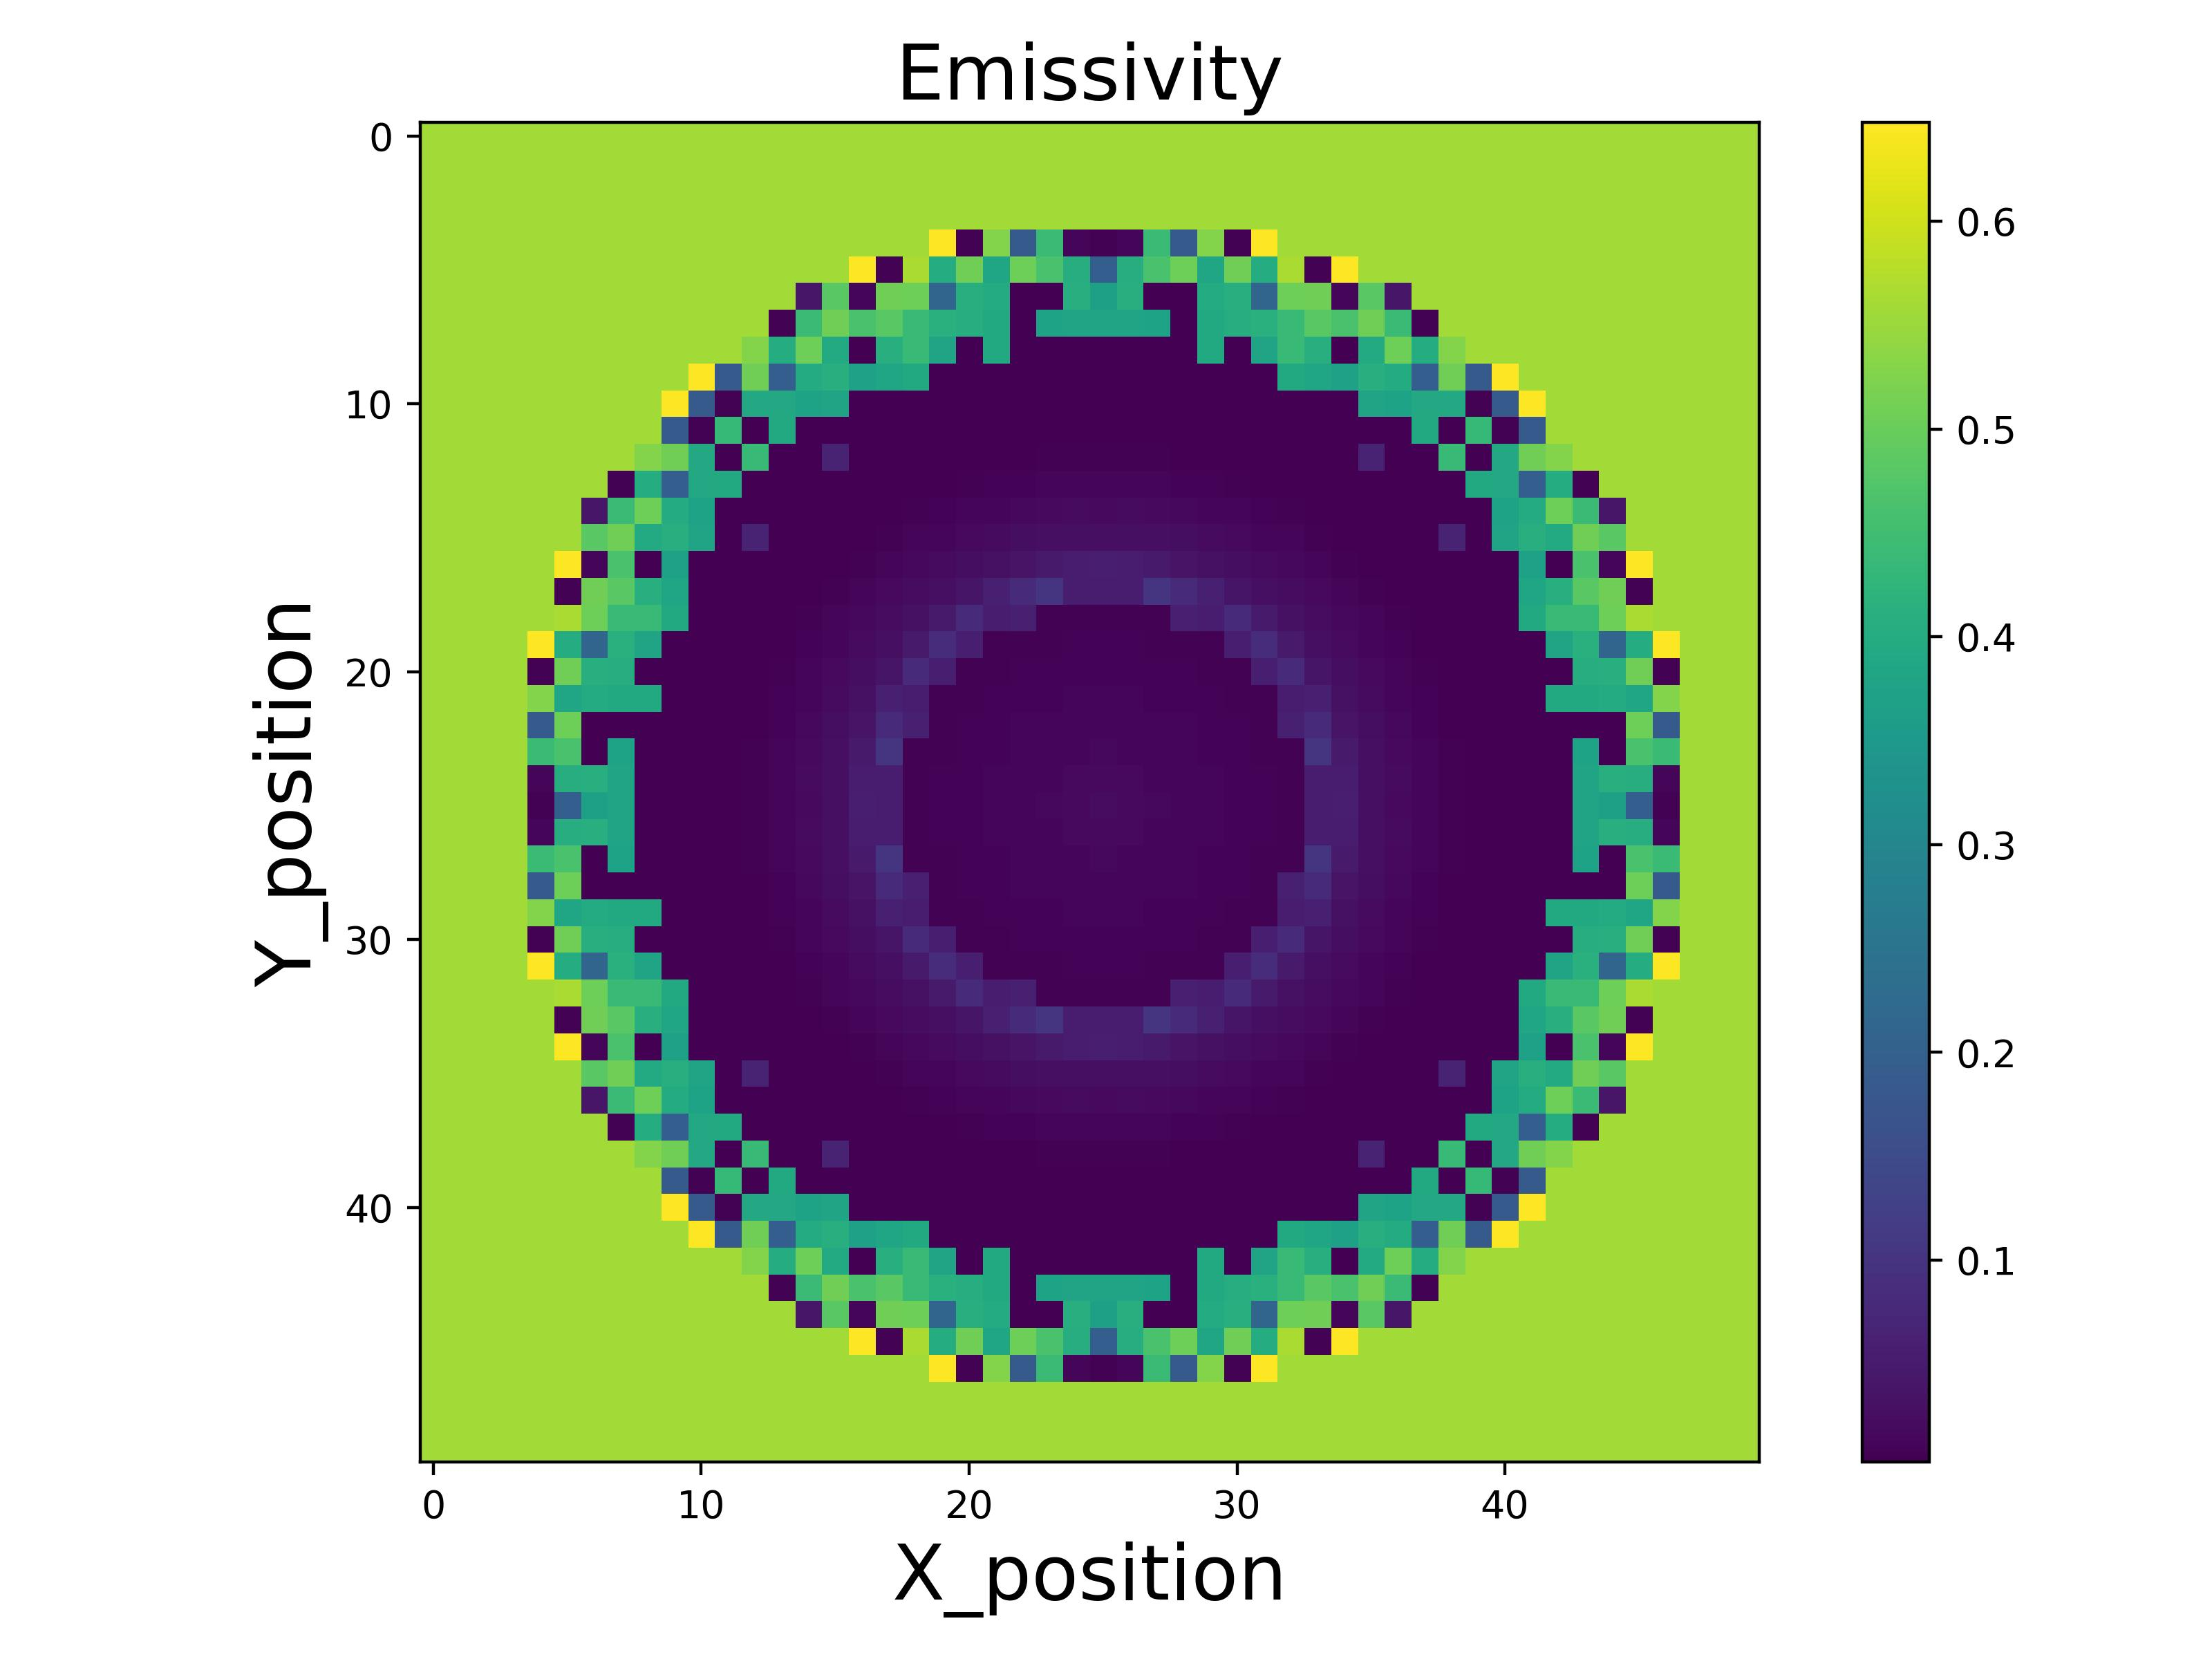
\includegraphics[width=\textwidth]{figures/raw_data/32/linear/emi_cal.jpg}
            \subcaption{Model 8}
        \end{subfigure}
        \begin{subfigure}{0.325\textwidth}
            \centering
            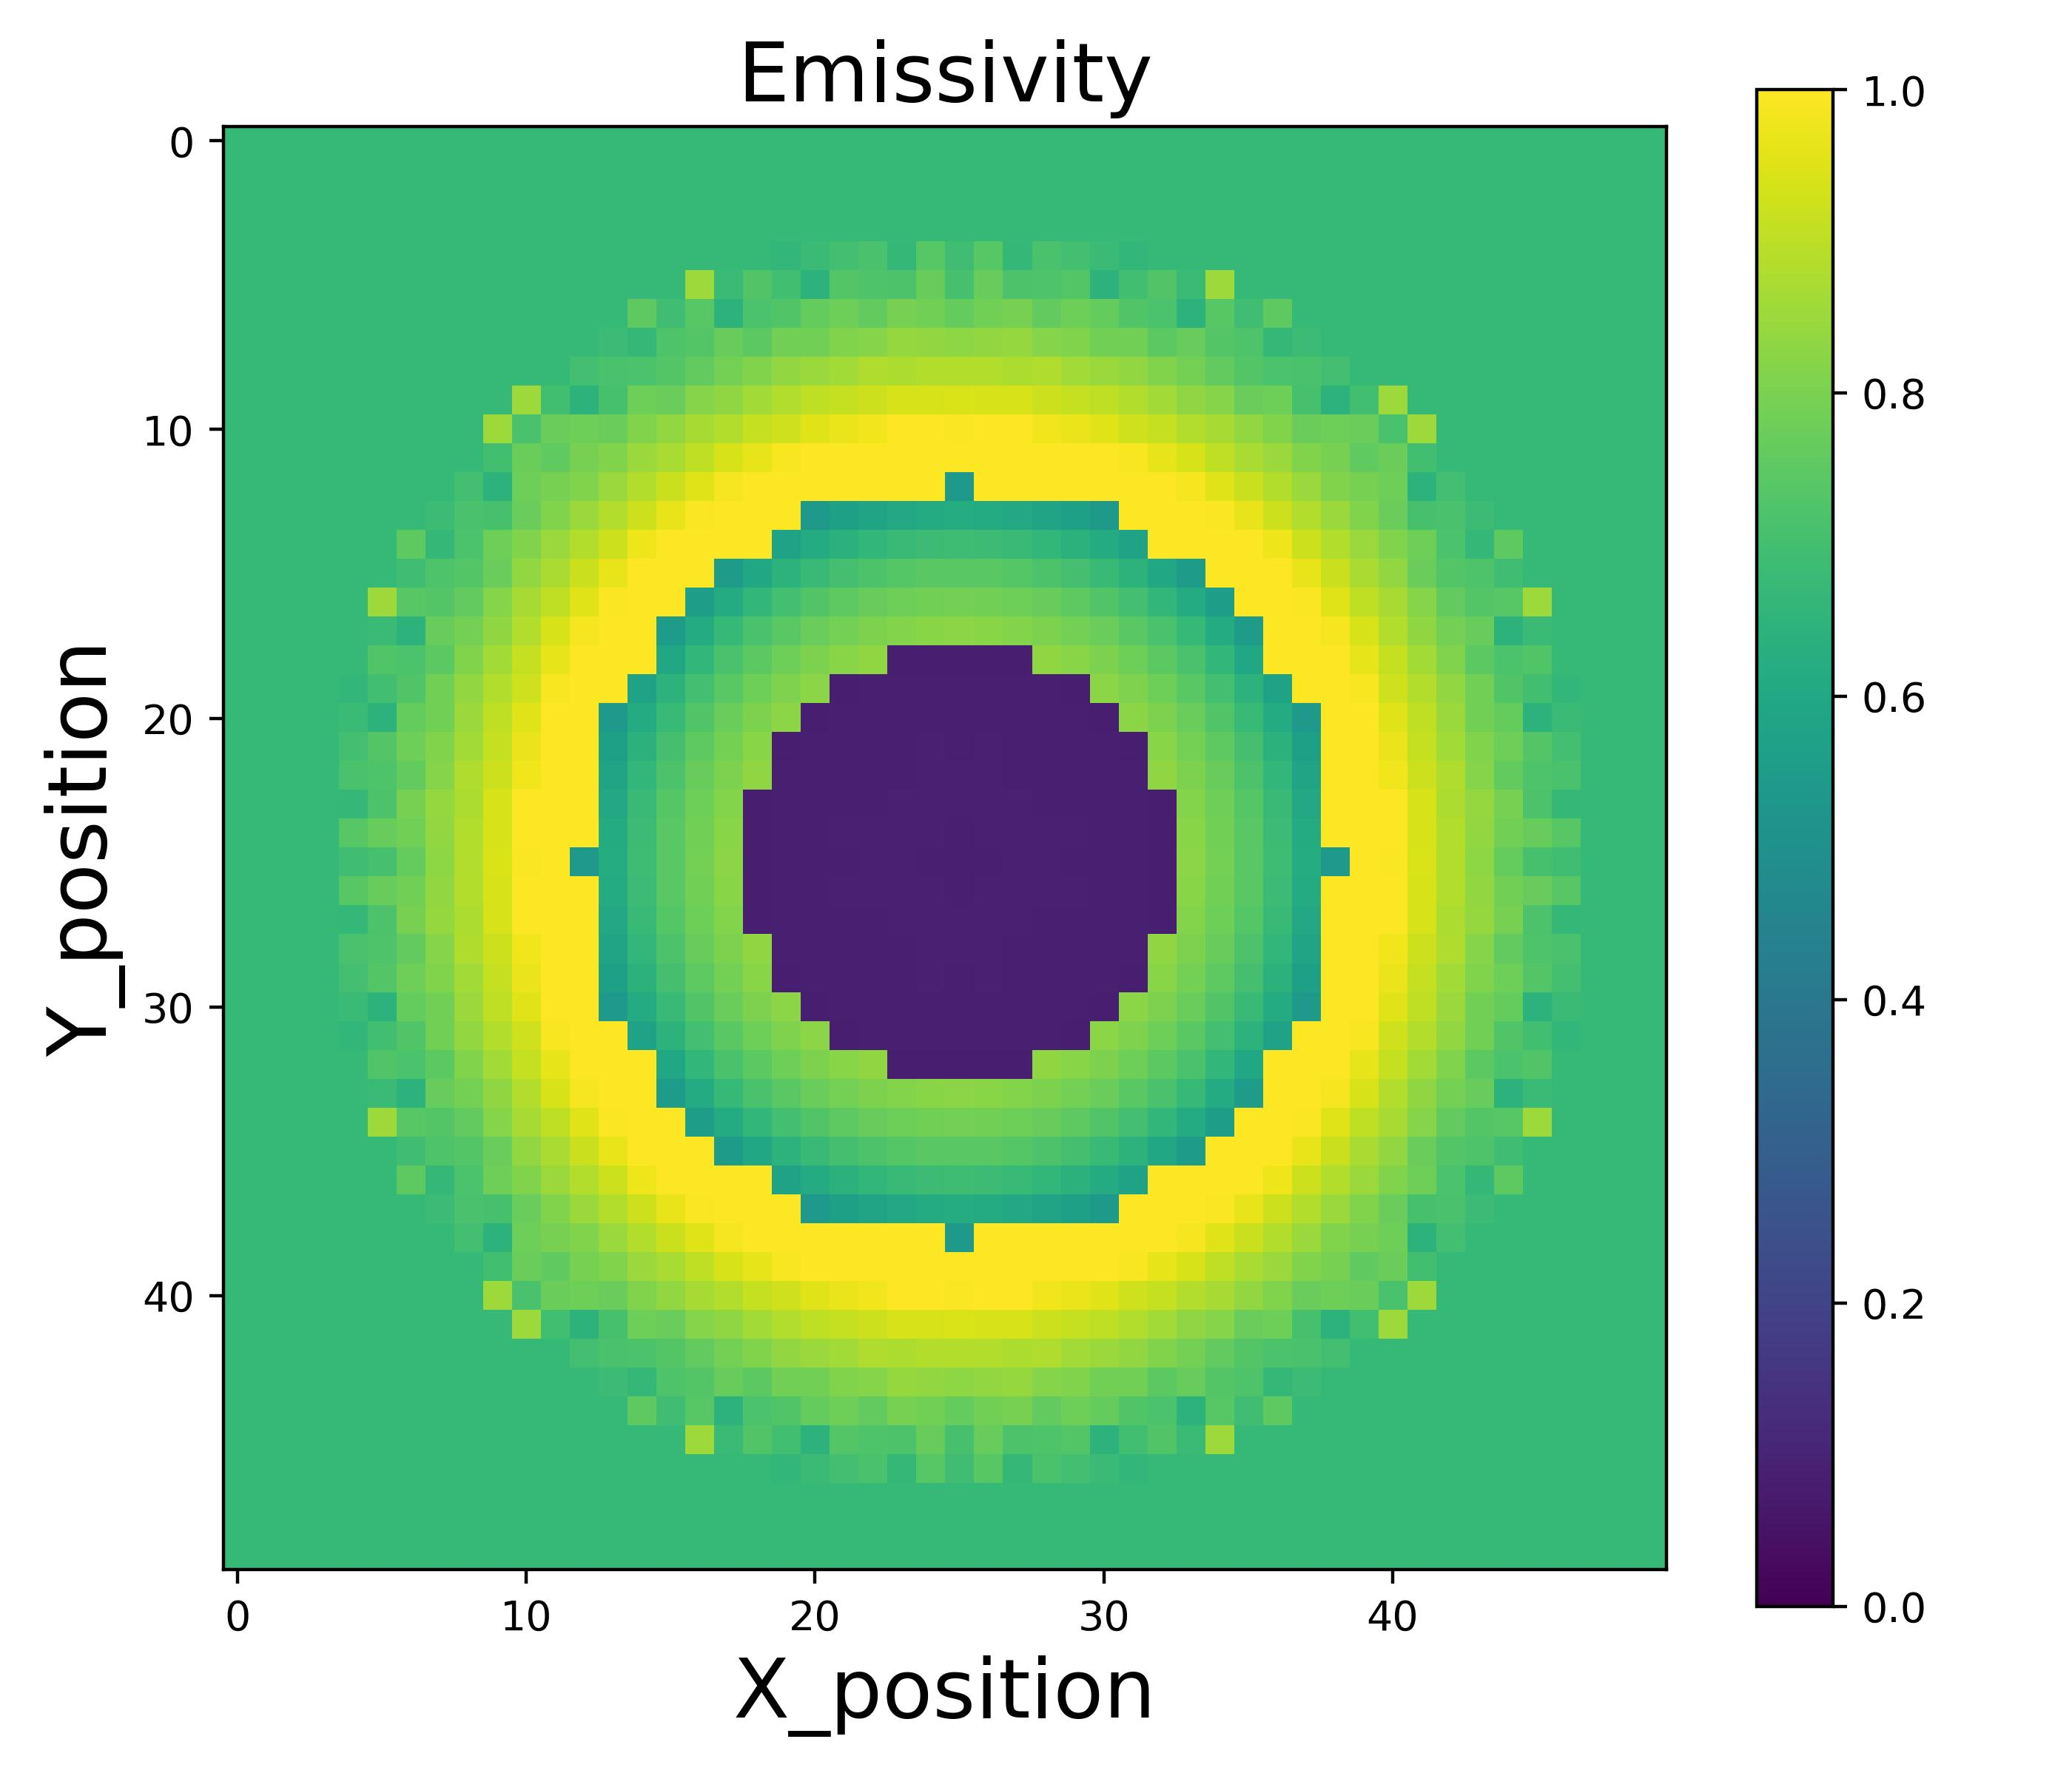
\includegraphics[width=\textwidth]{figures/raw_data/33/linear/emi_cal.jpg}
            \subcaption{Model 9}
        \end{subfigure}
    \end{minipage}
    \caption{Emissivity calculation results of linear model}  
\end{figure}


\newpage
\subsection{Linear square model}
\begin{figure}[h]
    \centering
    \begin{minipage}{\textwidth}
        \centering
        \begin{subfigure}{0.325\textwidth}
            \centering
            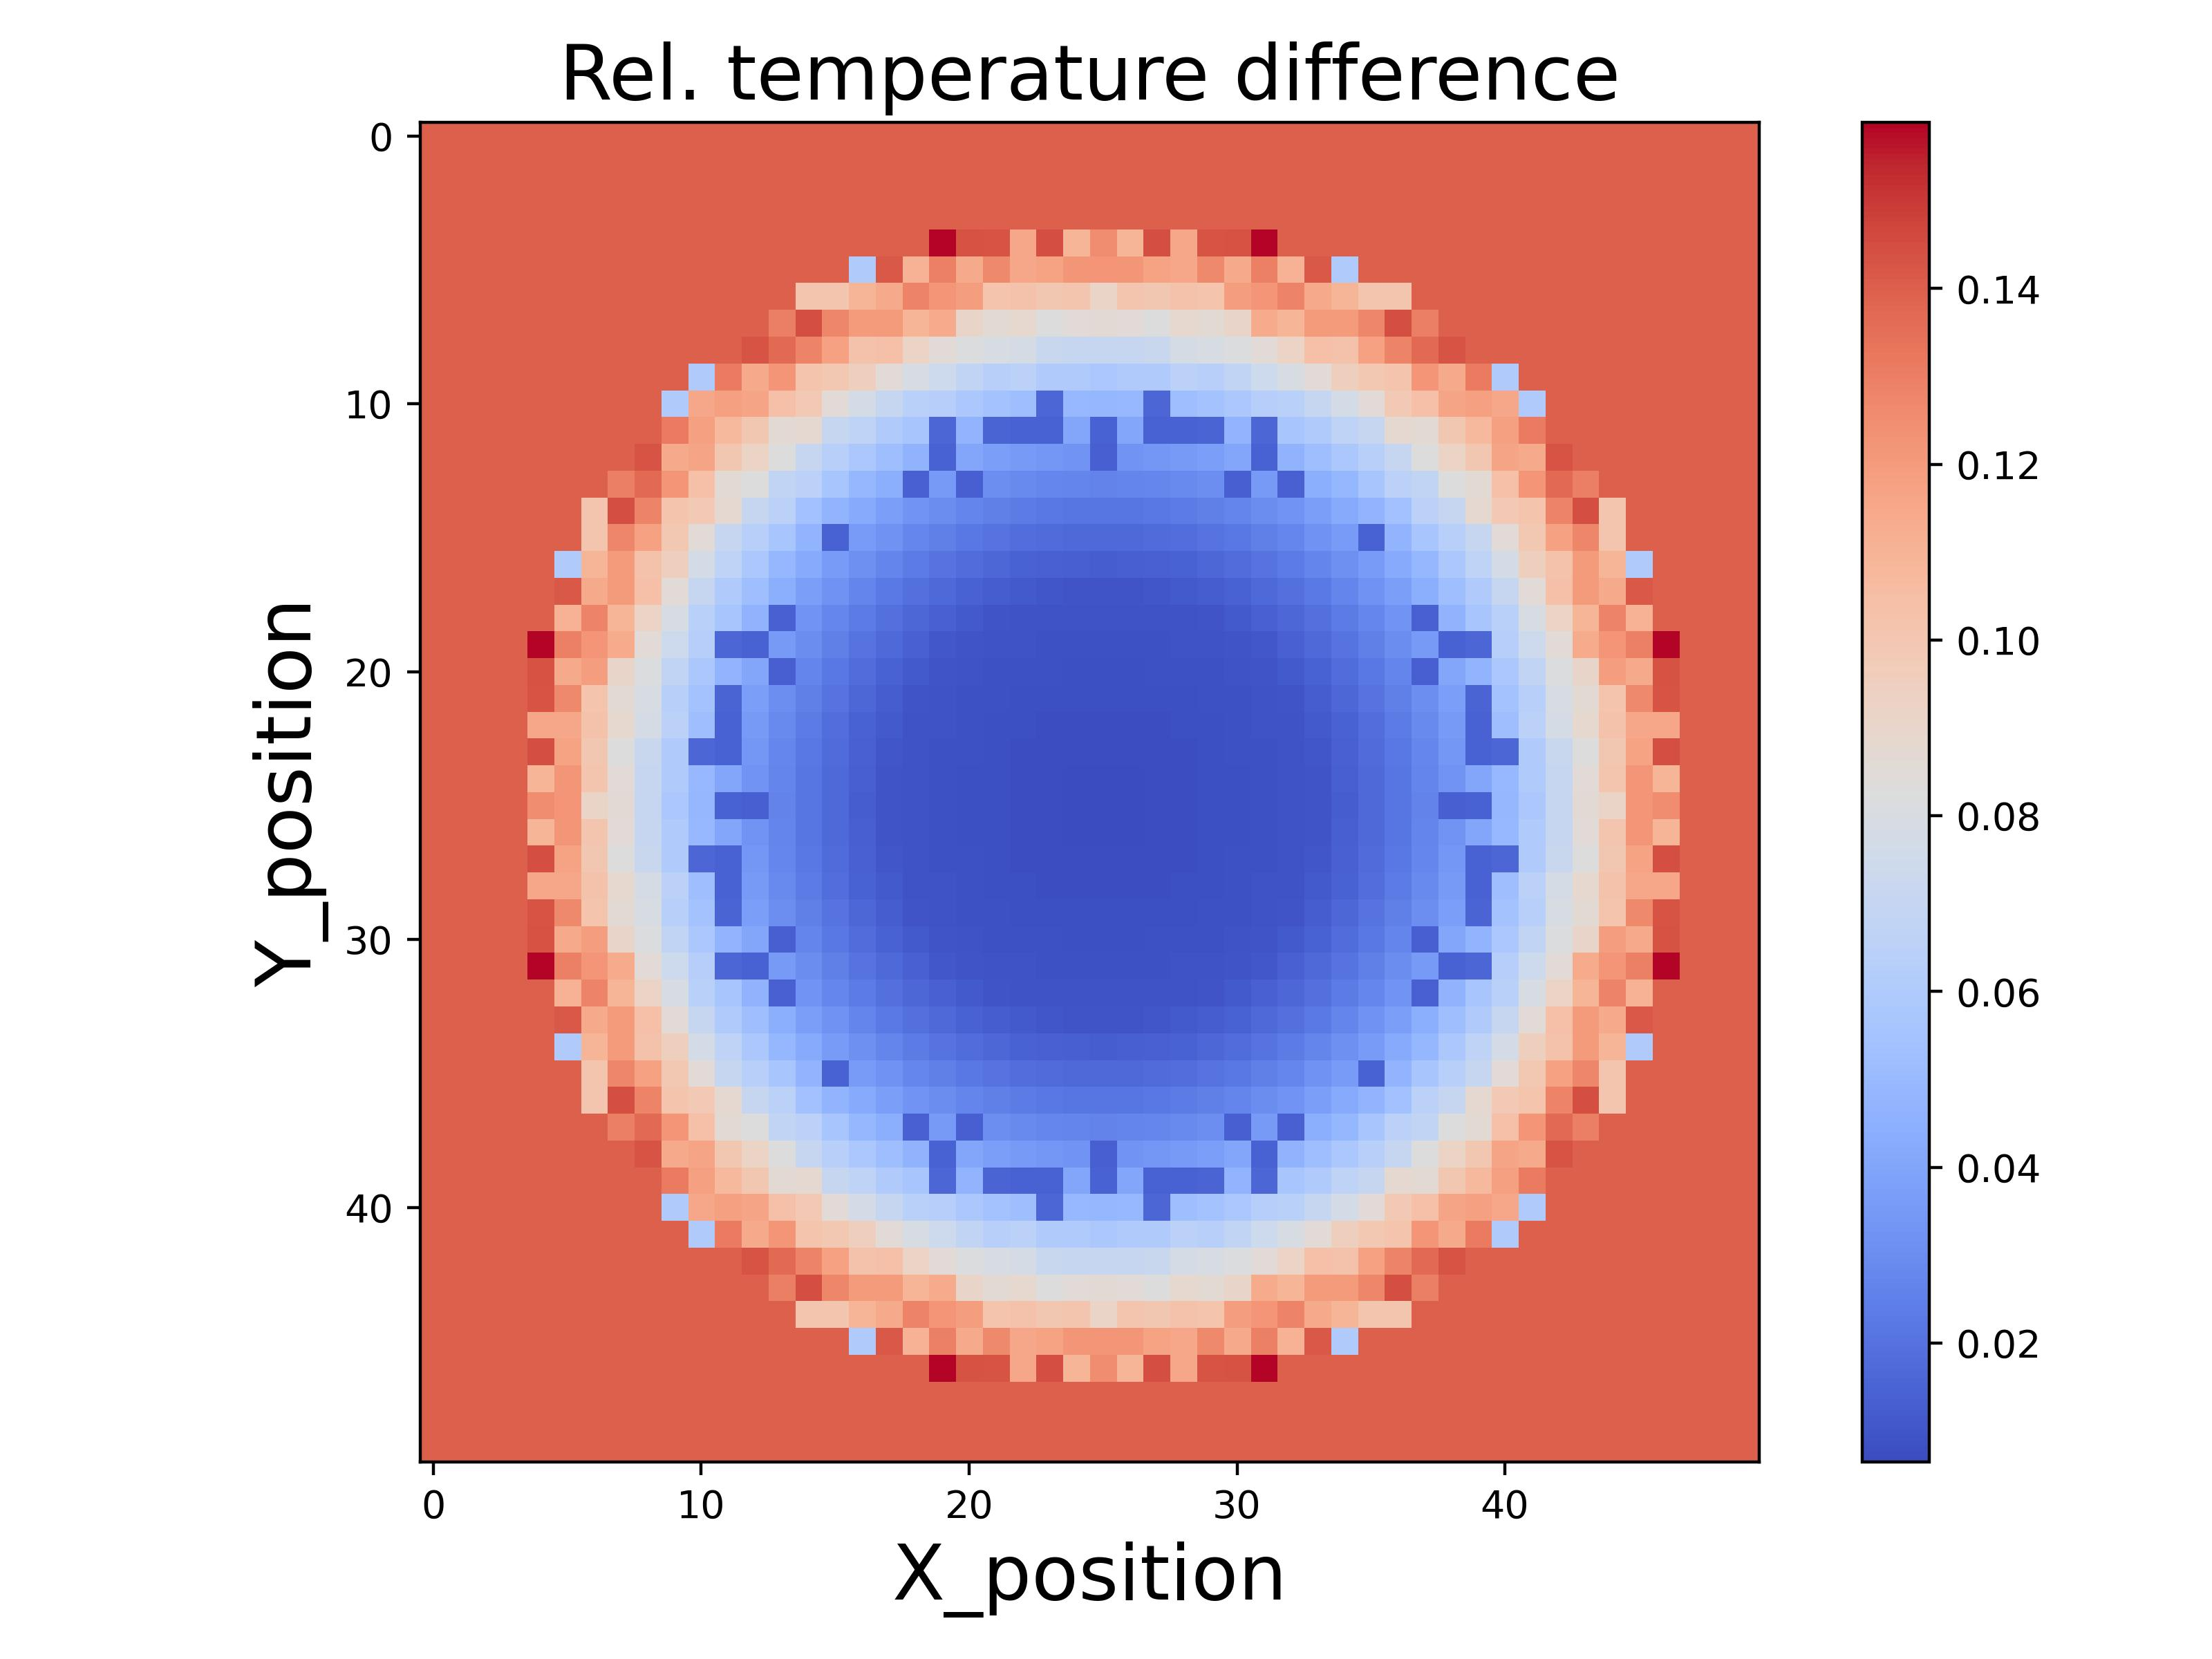
\includegraphics[width=\textwidth]{figures/raw_data/0/lin_square/T_bias.jpg}
            \subcaption{Black body material}
        \end{subfigure}
        \begin{subfigure}{0.325\textwidth}
            \centering
            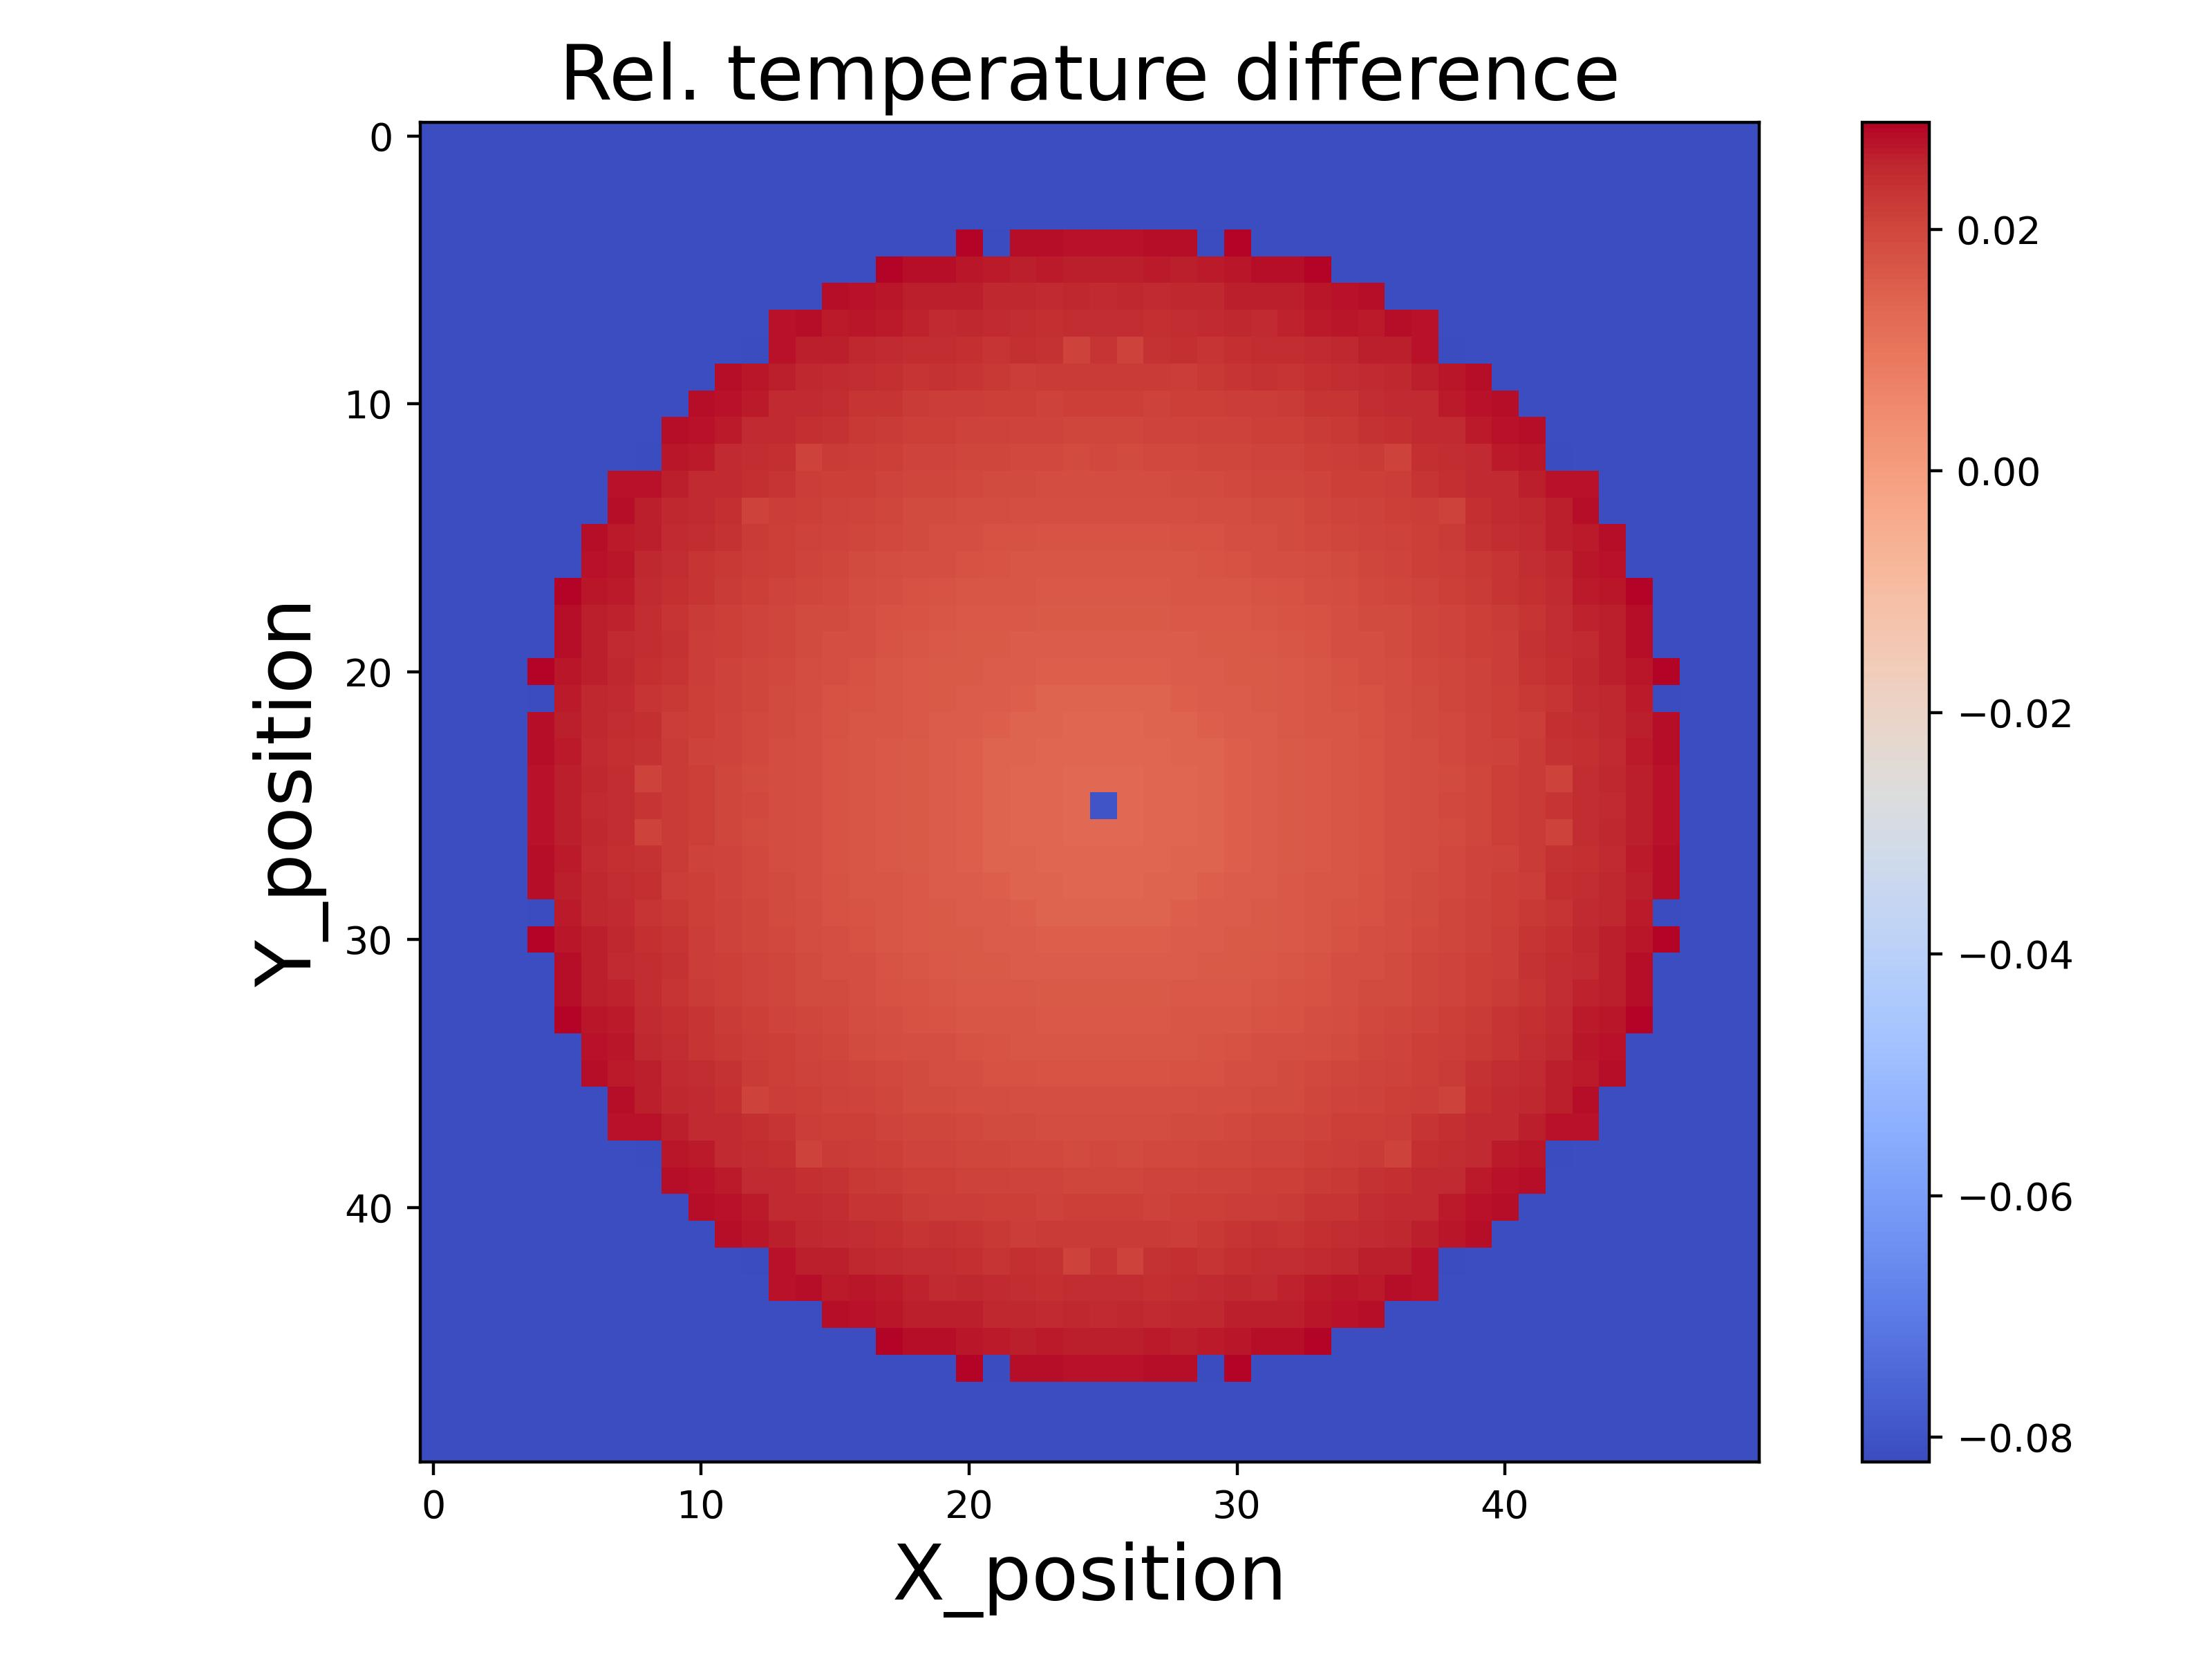
\includegraphics[width=\textwidth]{figures/raw_data/5/lin_square/T_bias.jpg}
            \subcaption{Real iron data}
        \end{subfigure}
        \begin{subfigure}{0.325\textwidth}
            \centering
            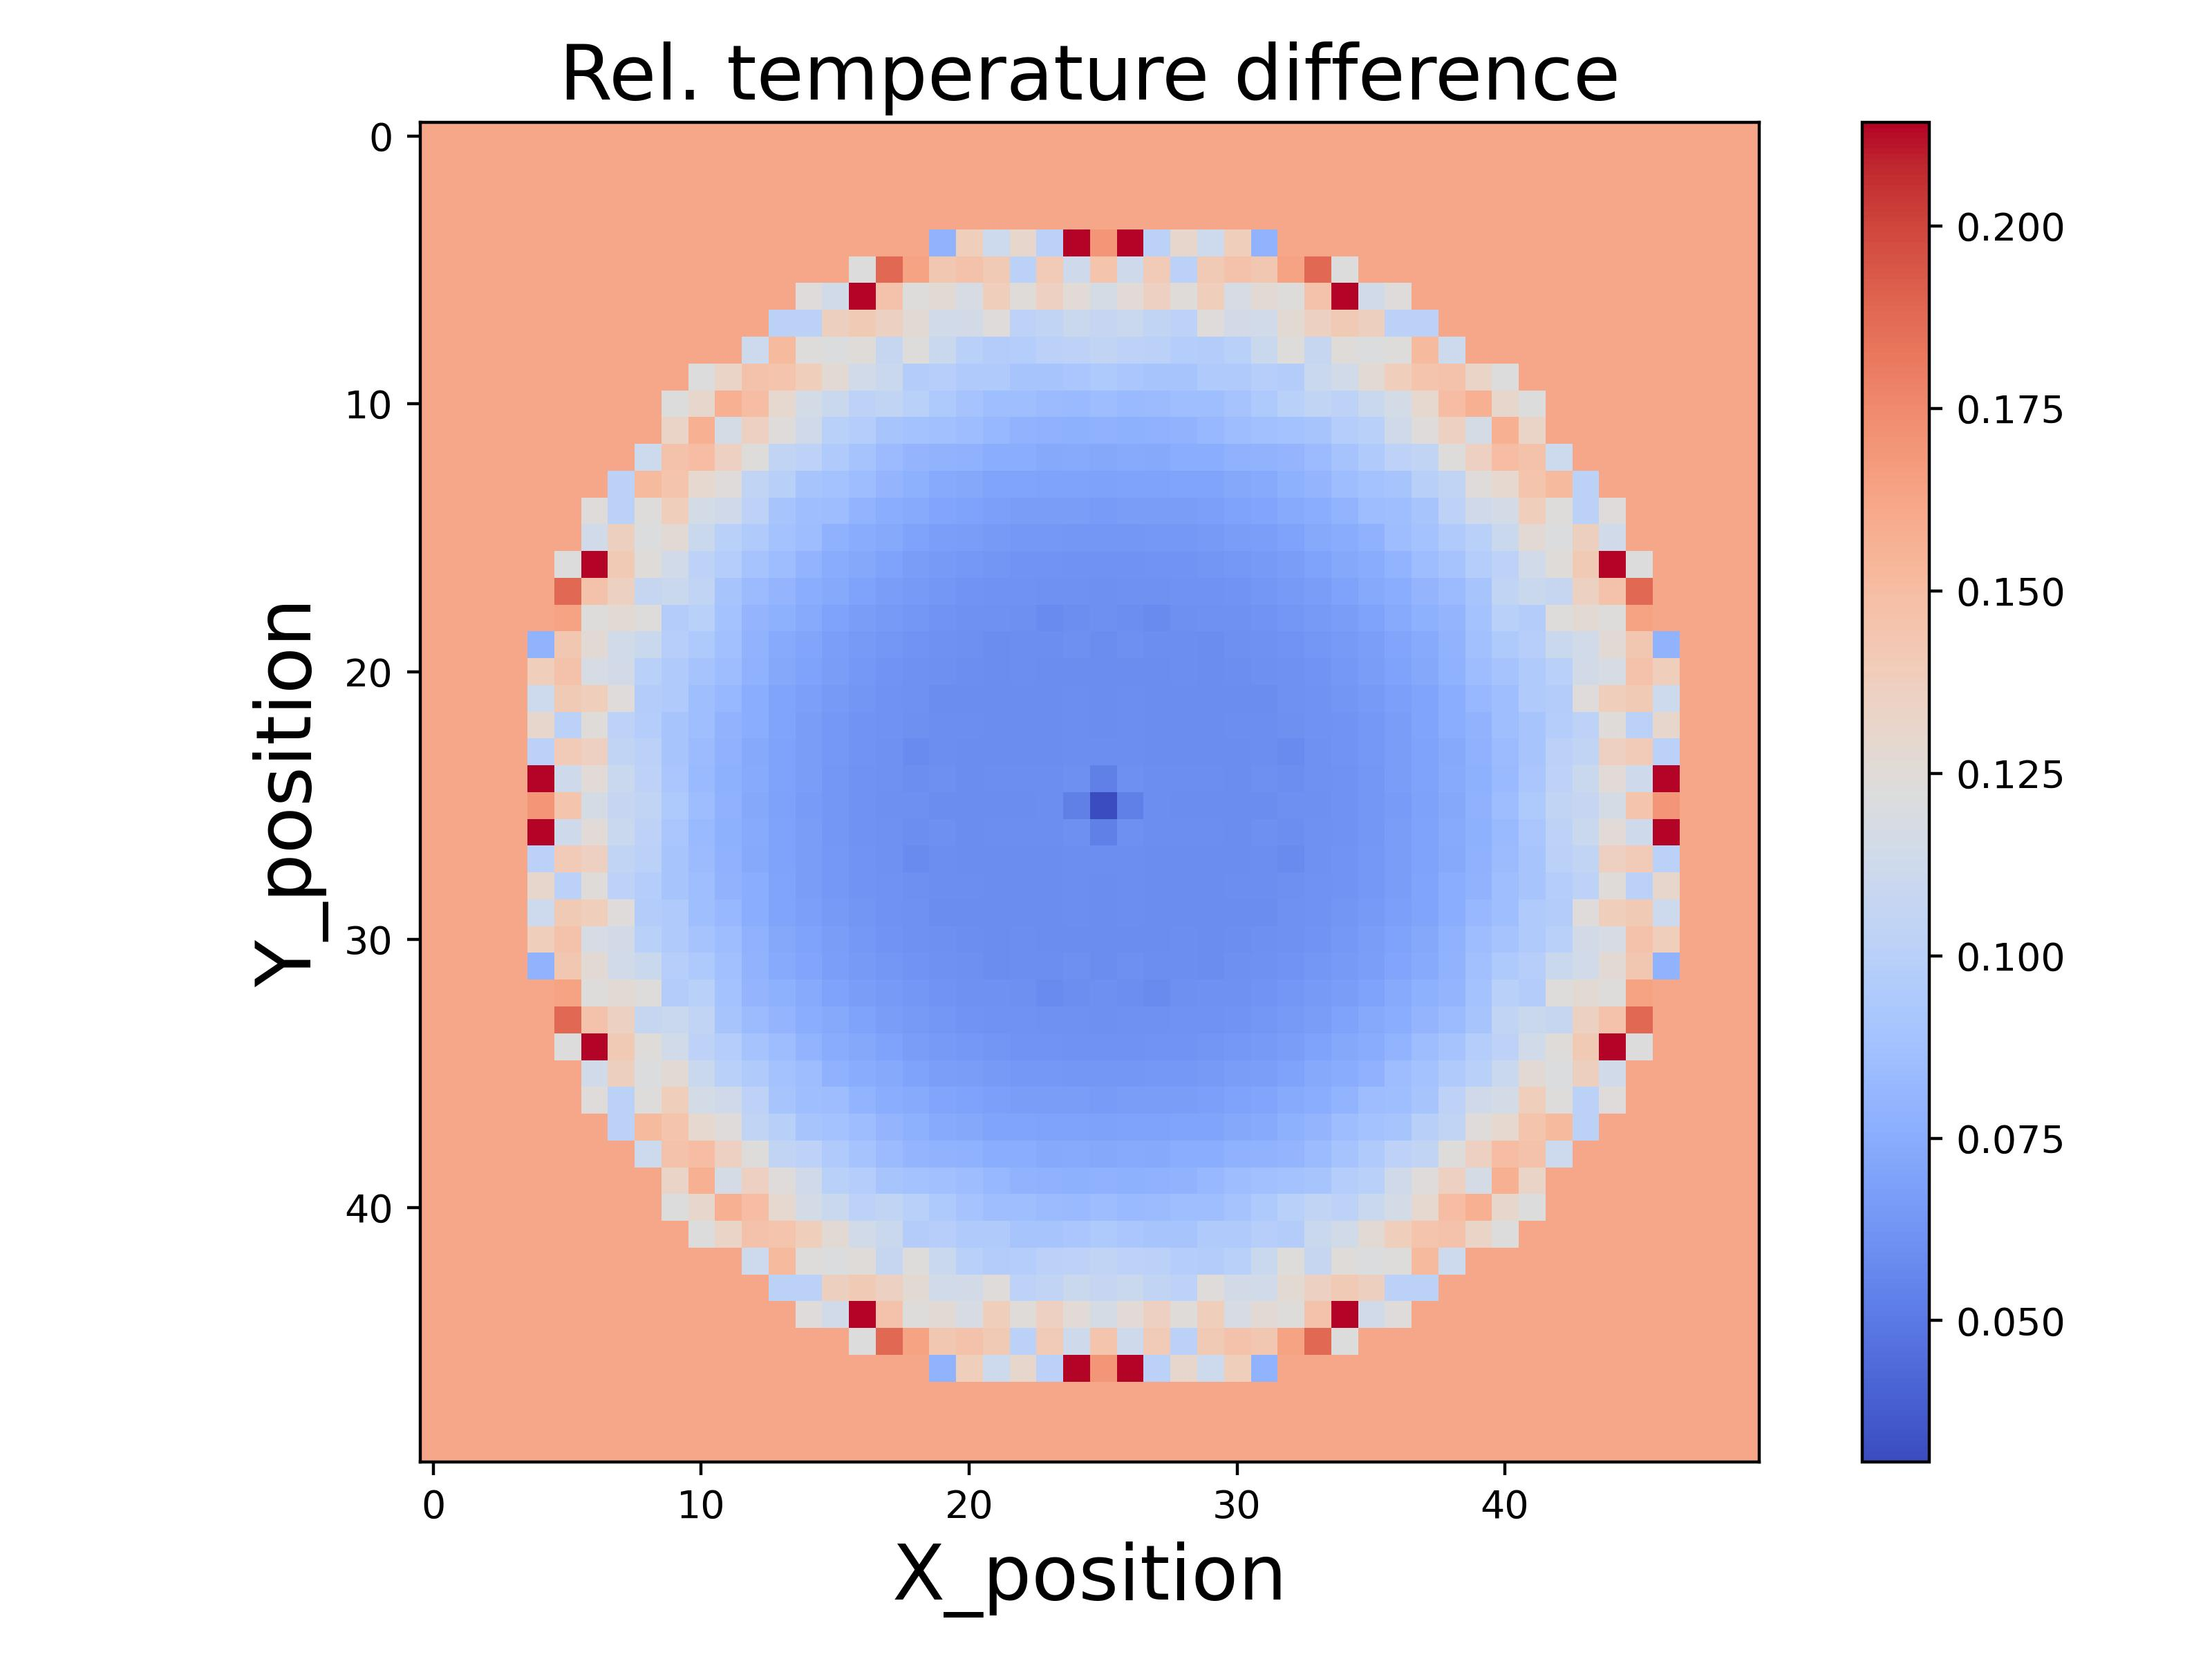
\includegraphics[width=\textwidth]{figures/raw_data/21/lin_square/T_bias.jpg}
            \subcaption{Model 1}
        \end{subfigure}
    \end{minipage}\\
    \begin{minipage}{\textwidth}
        \centering
        \begin{subfigure}{0.325\textwidth}
            \centering
            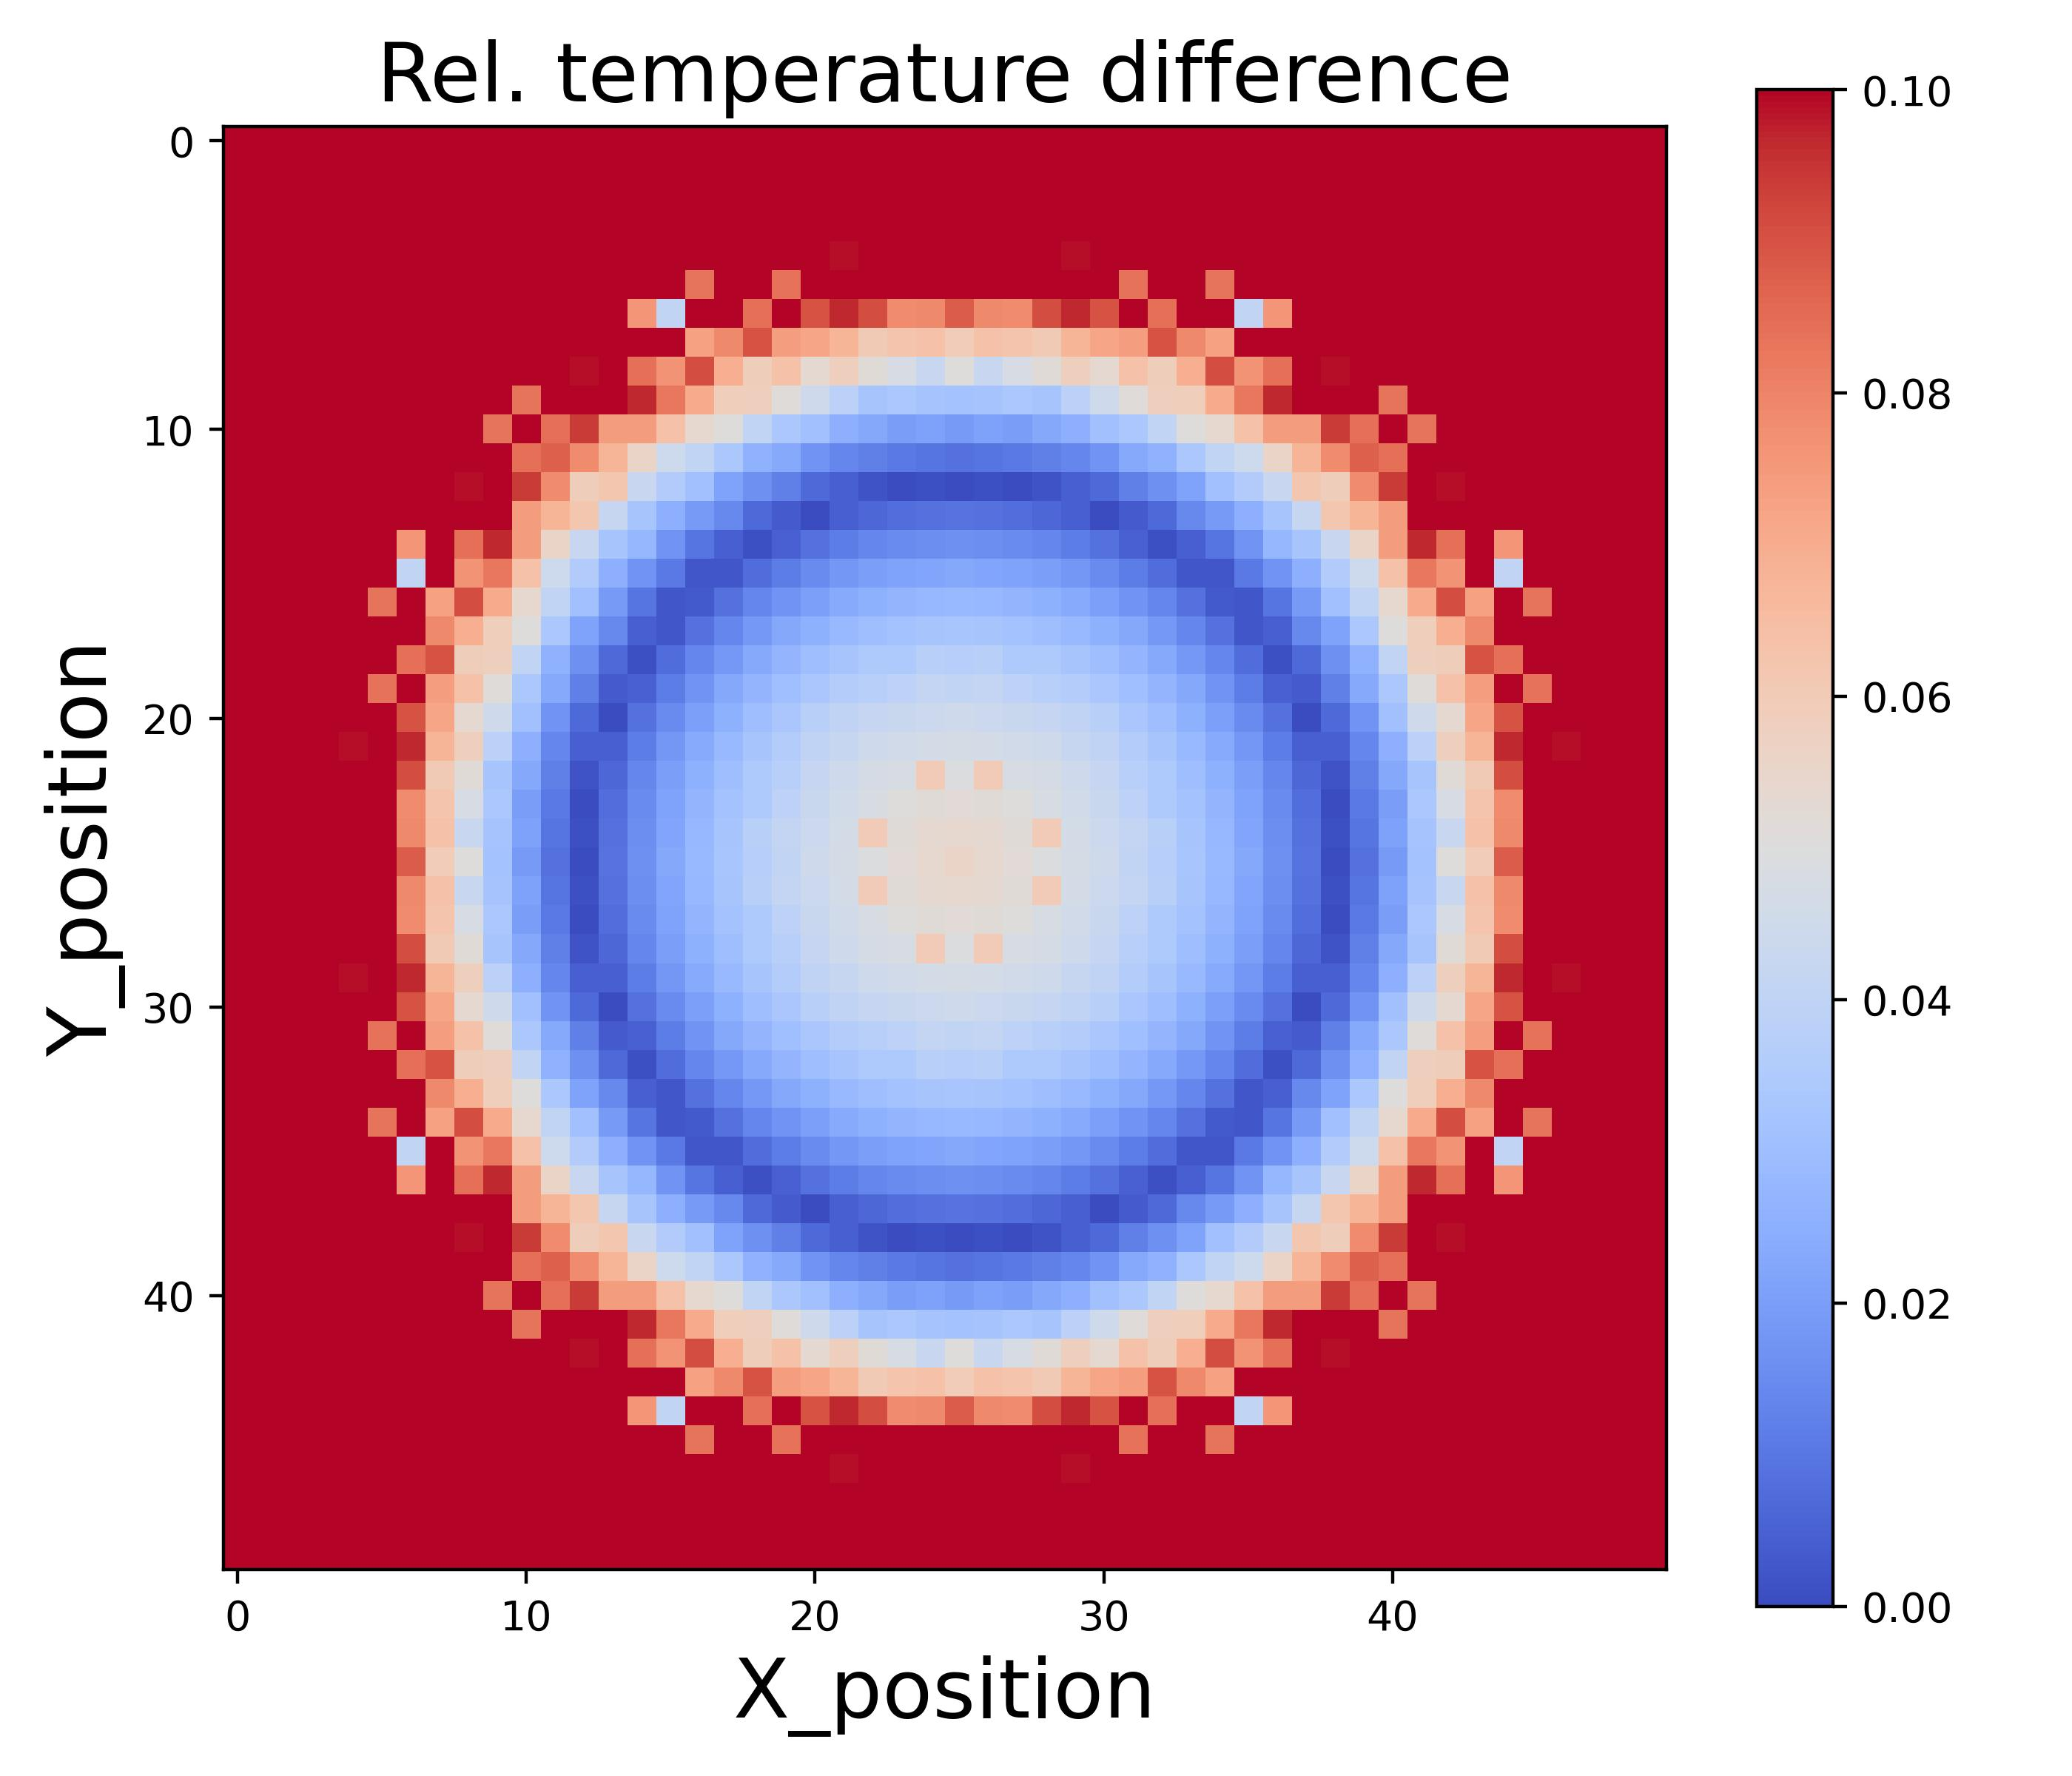
\includegraphics[width=\textwidth]{figures/raw_data/22/lin_square/T_bias.jpg}
            \subcaption{Model 2}
        \end{subfigure}
        \begin{subfigure}{0.325\textwidth}
            \centering
            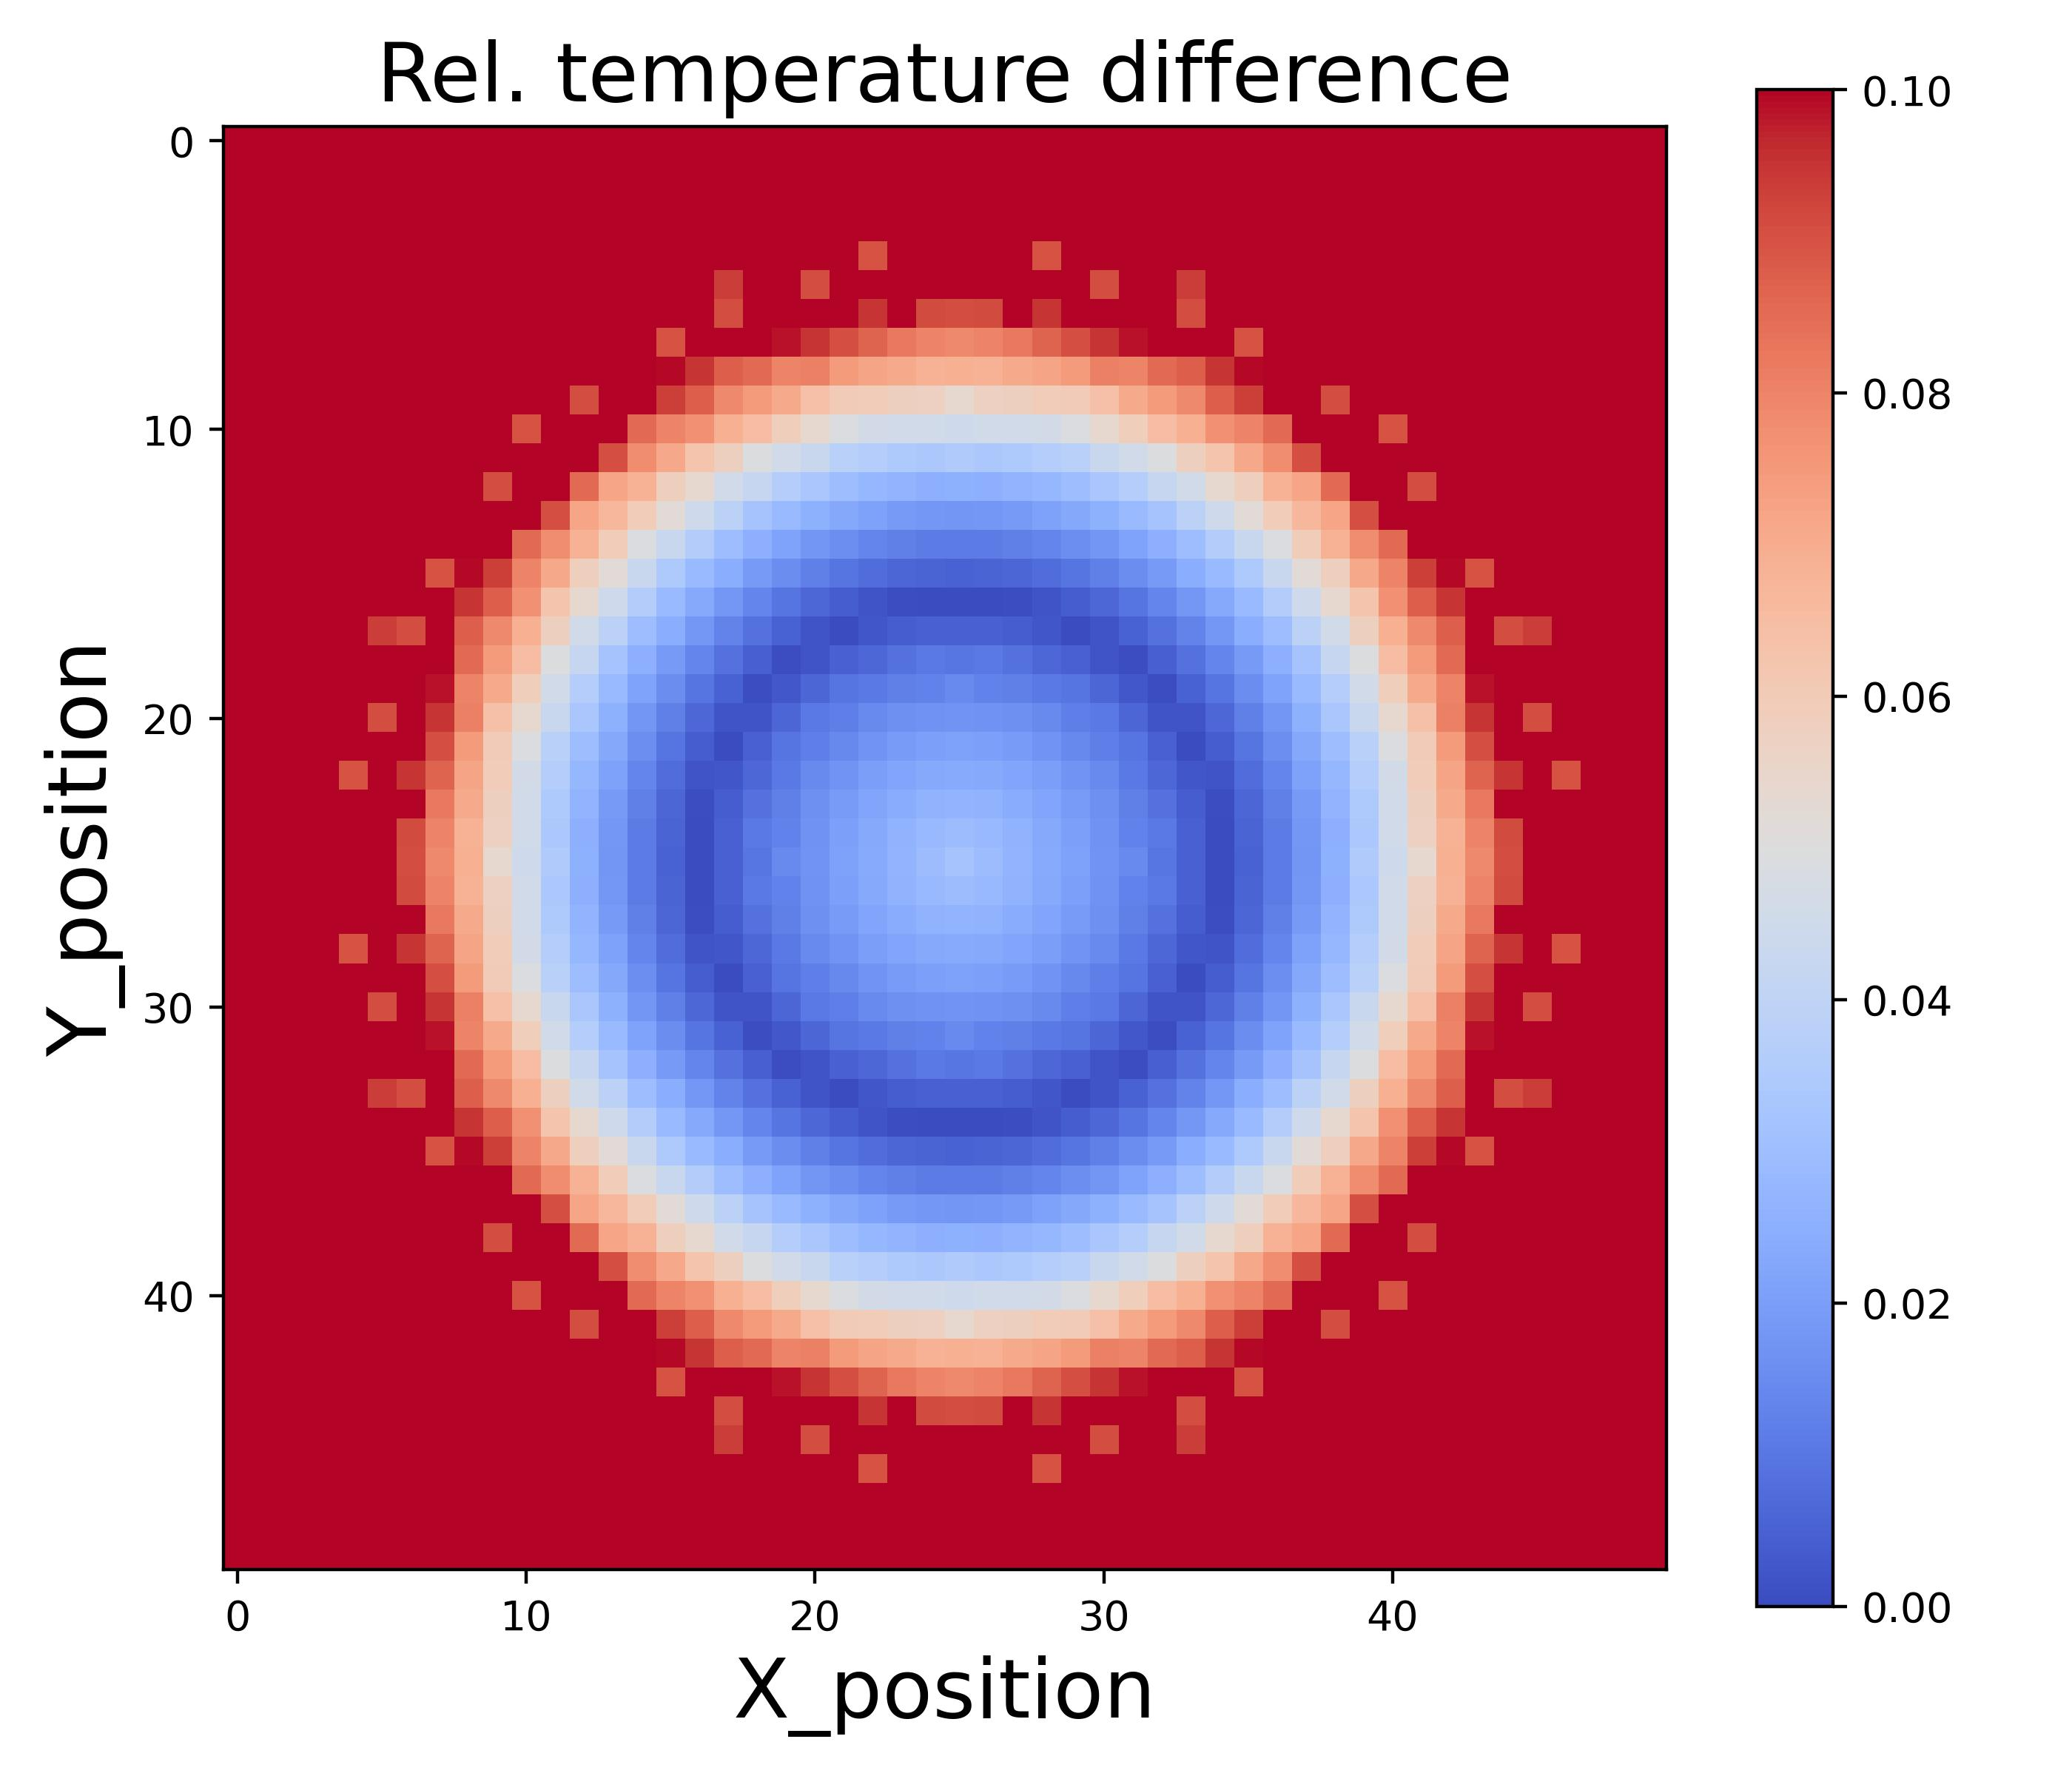
\includegraphics[width=\textwidth]{figures/raw_data/23/lin_square/T_bias.jpg}
            \subcaption{Model 3}
        \end{subfigure}
        \begin{subfigure}{0.325\textwidth}
            \centering
            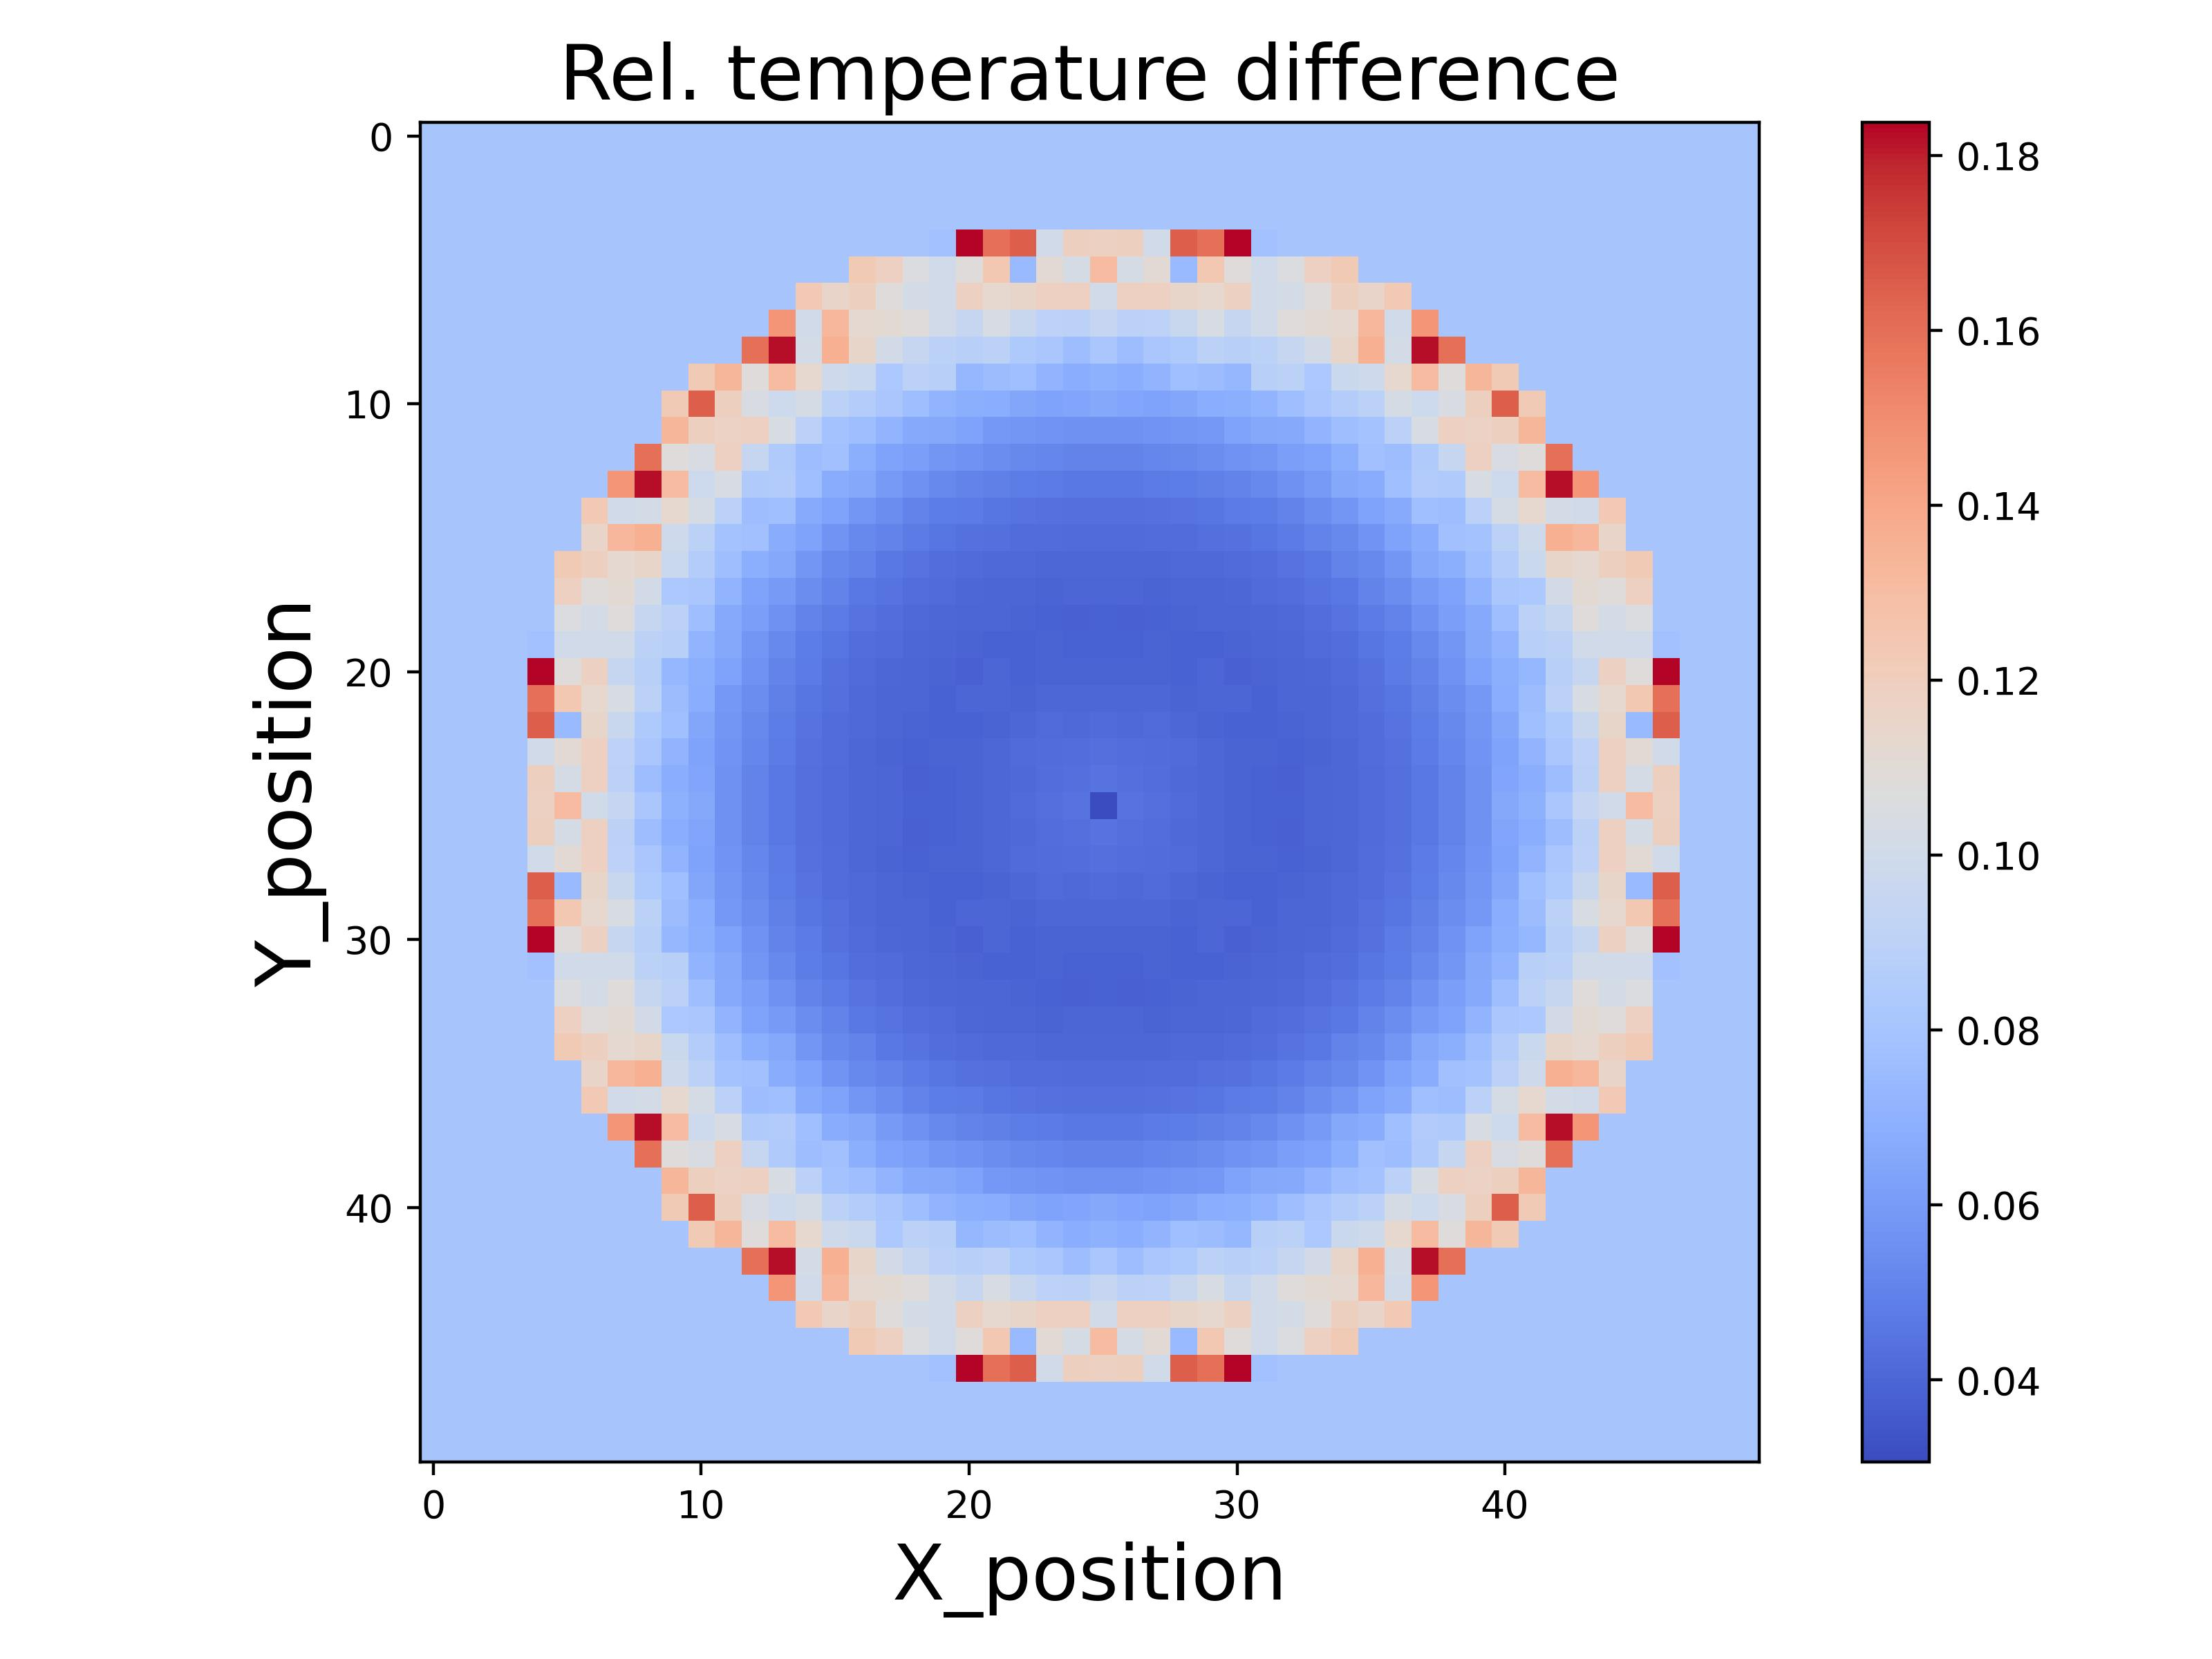
\includegraphics[width=\textwidth]{figures/raw_data/24/lin_square/T_bias.jpg}
            \subcaption{Model 4}
        \end{subfigure}
    \end{minipage}\\
    \begin{minipage}{\textwidth}
        \centering
        \begin{subfigure}{0.325\textwidth}
            \centering
            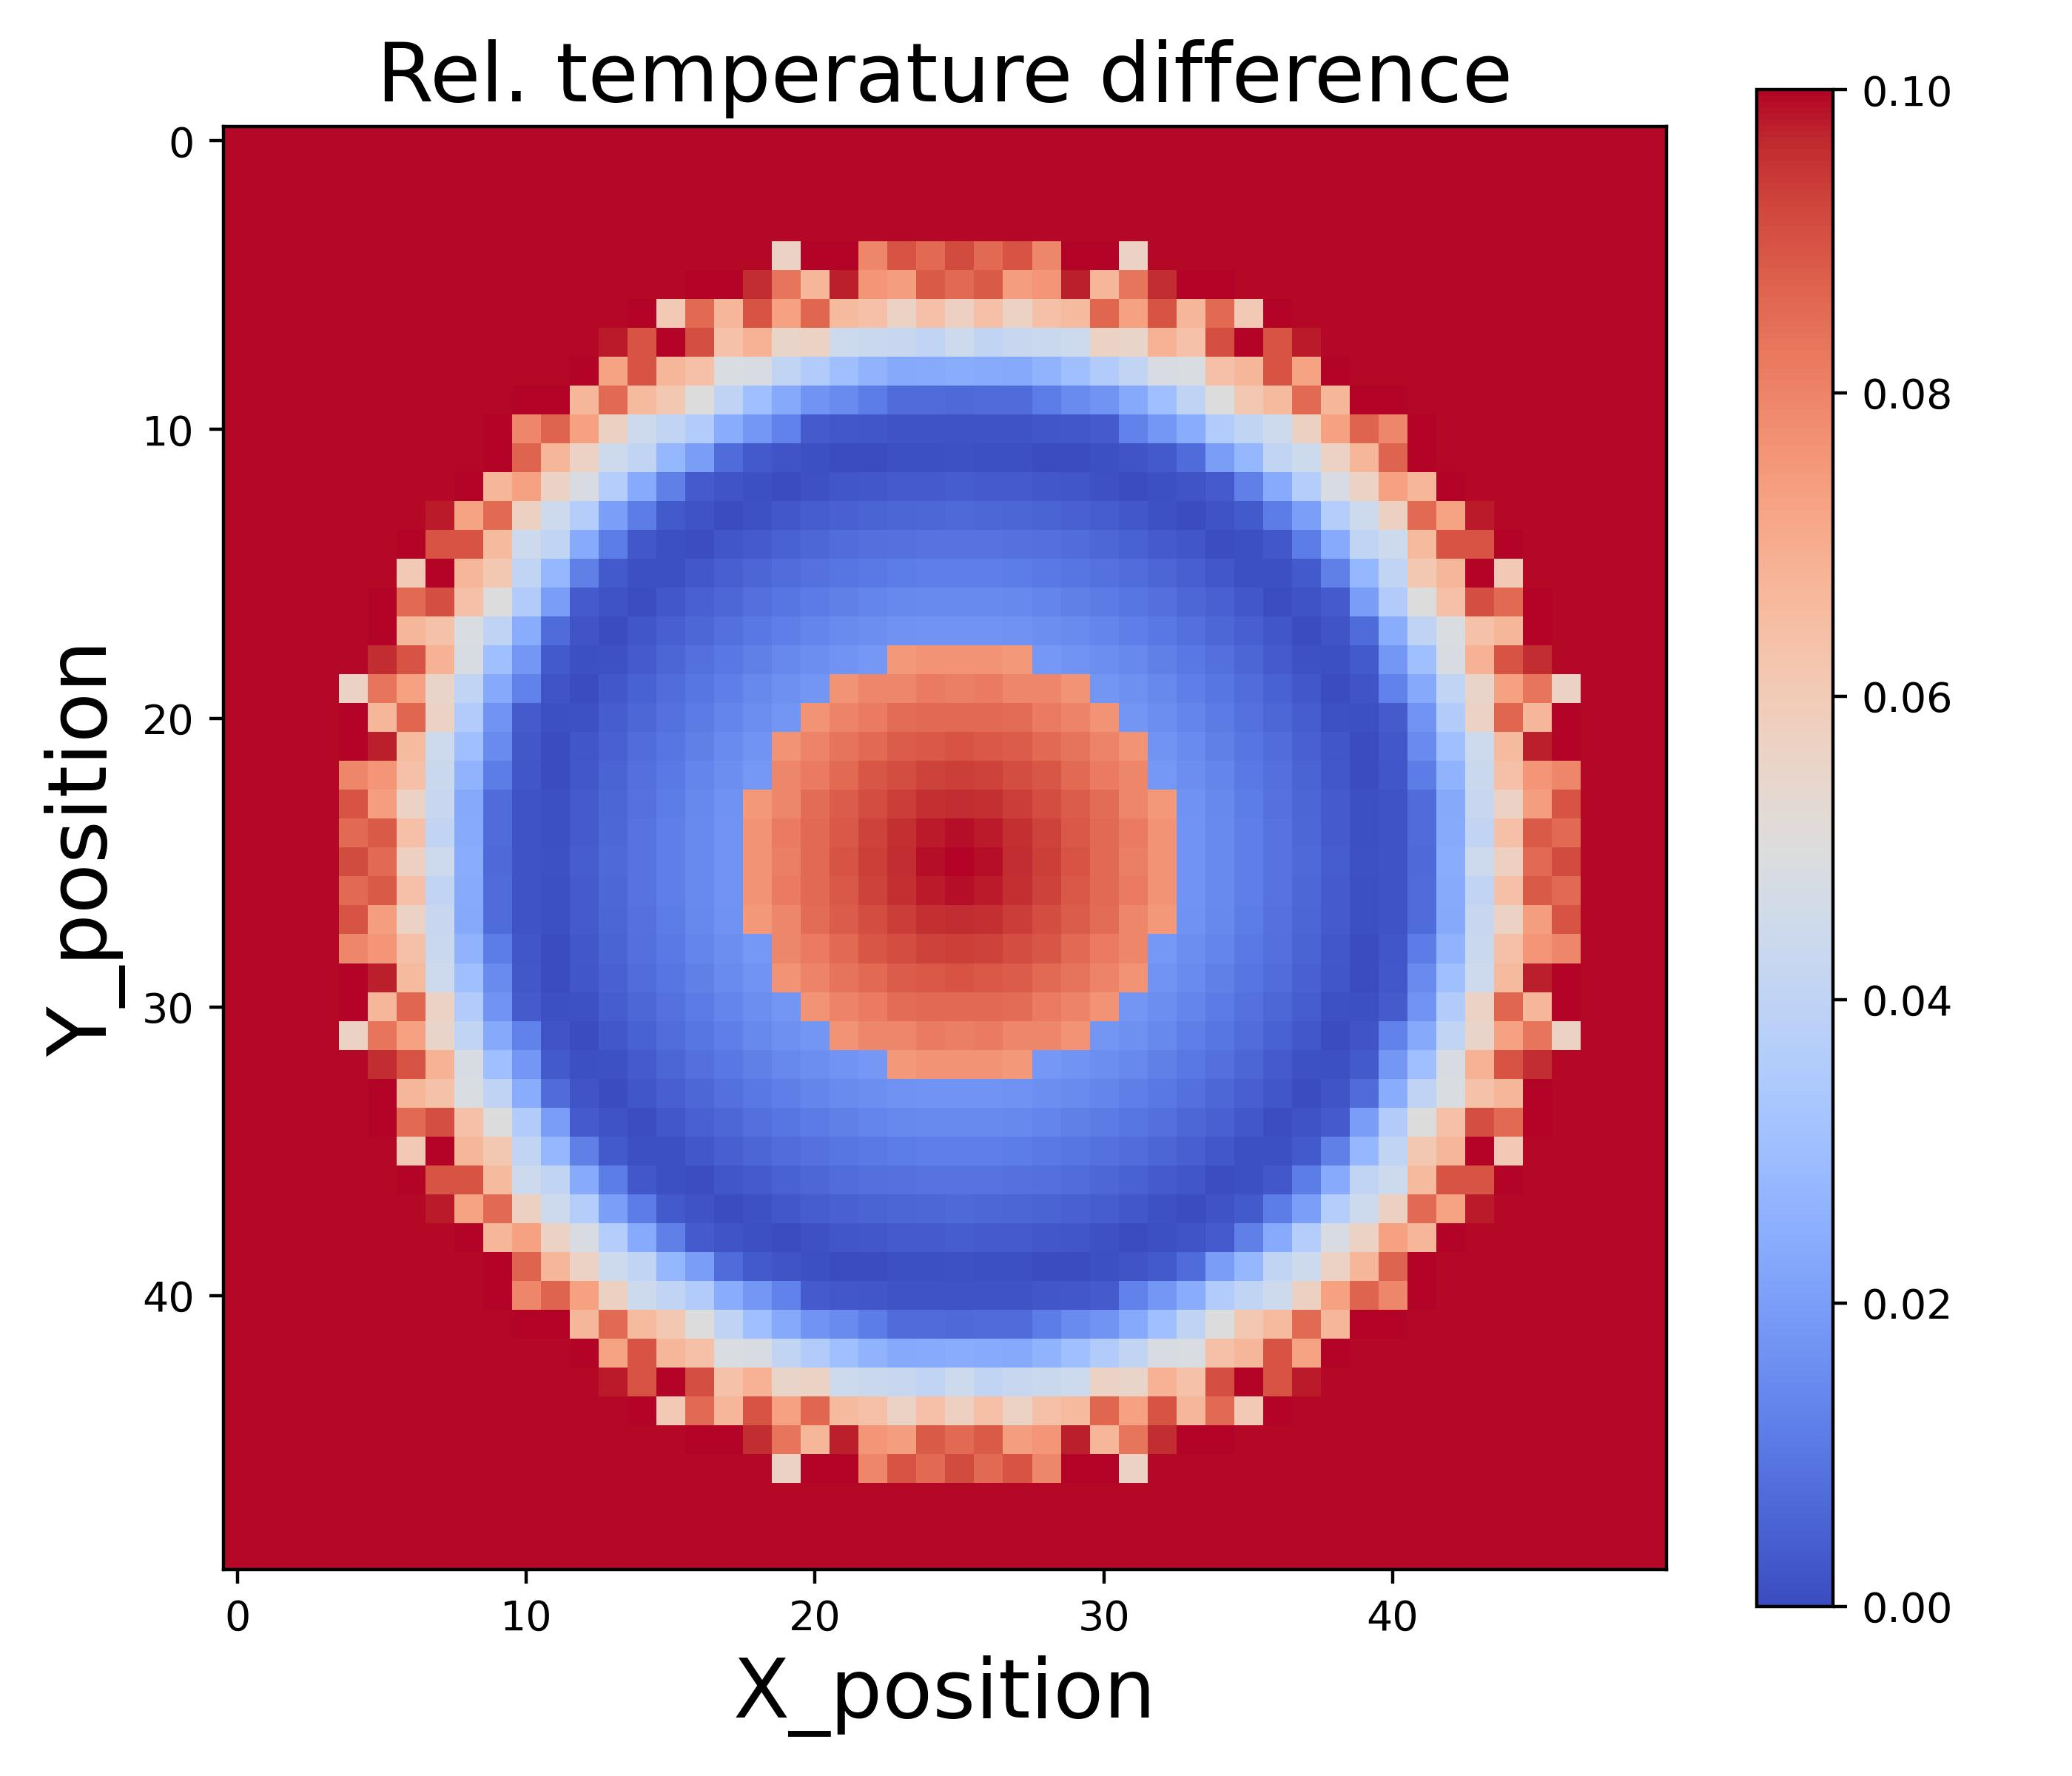
\includegraphics[width=\textwidth]{figures/raw_data/25/lin_square/T_bias.jpg}
            \subcaption{Model 5}
        \end{subfigure}
        \begin{subfigure}{0.325\textwidth}
            \centering
            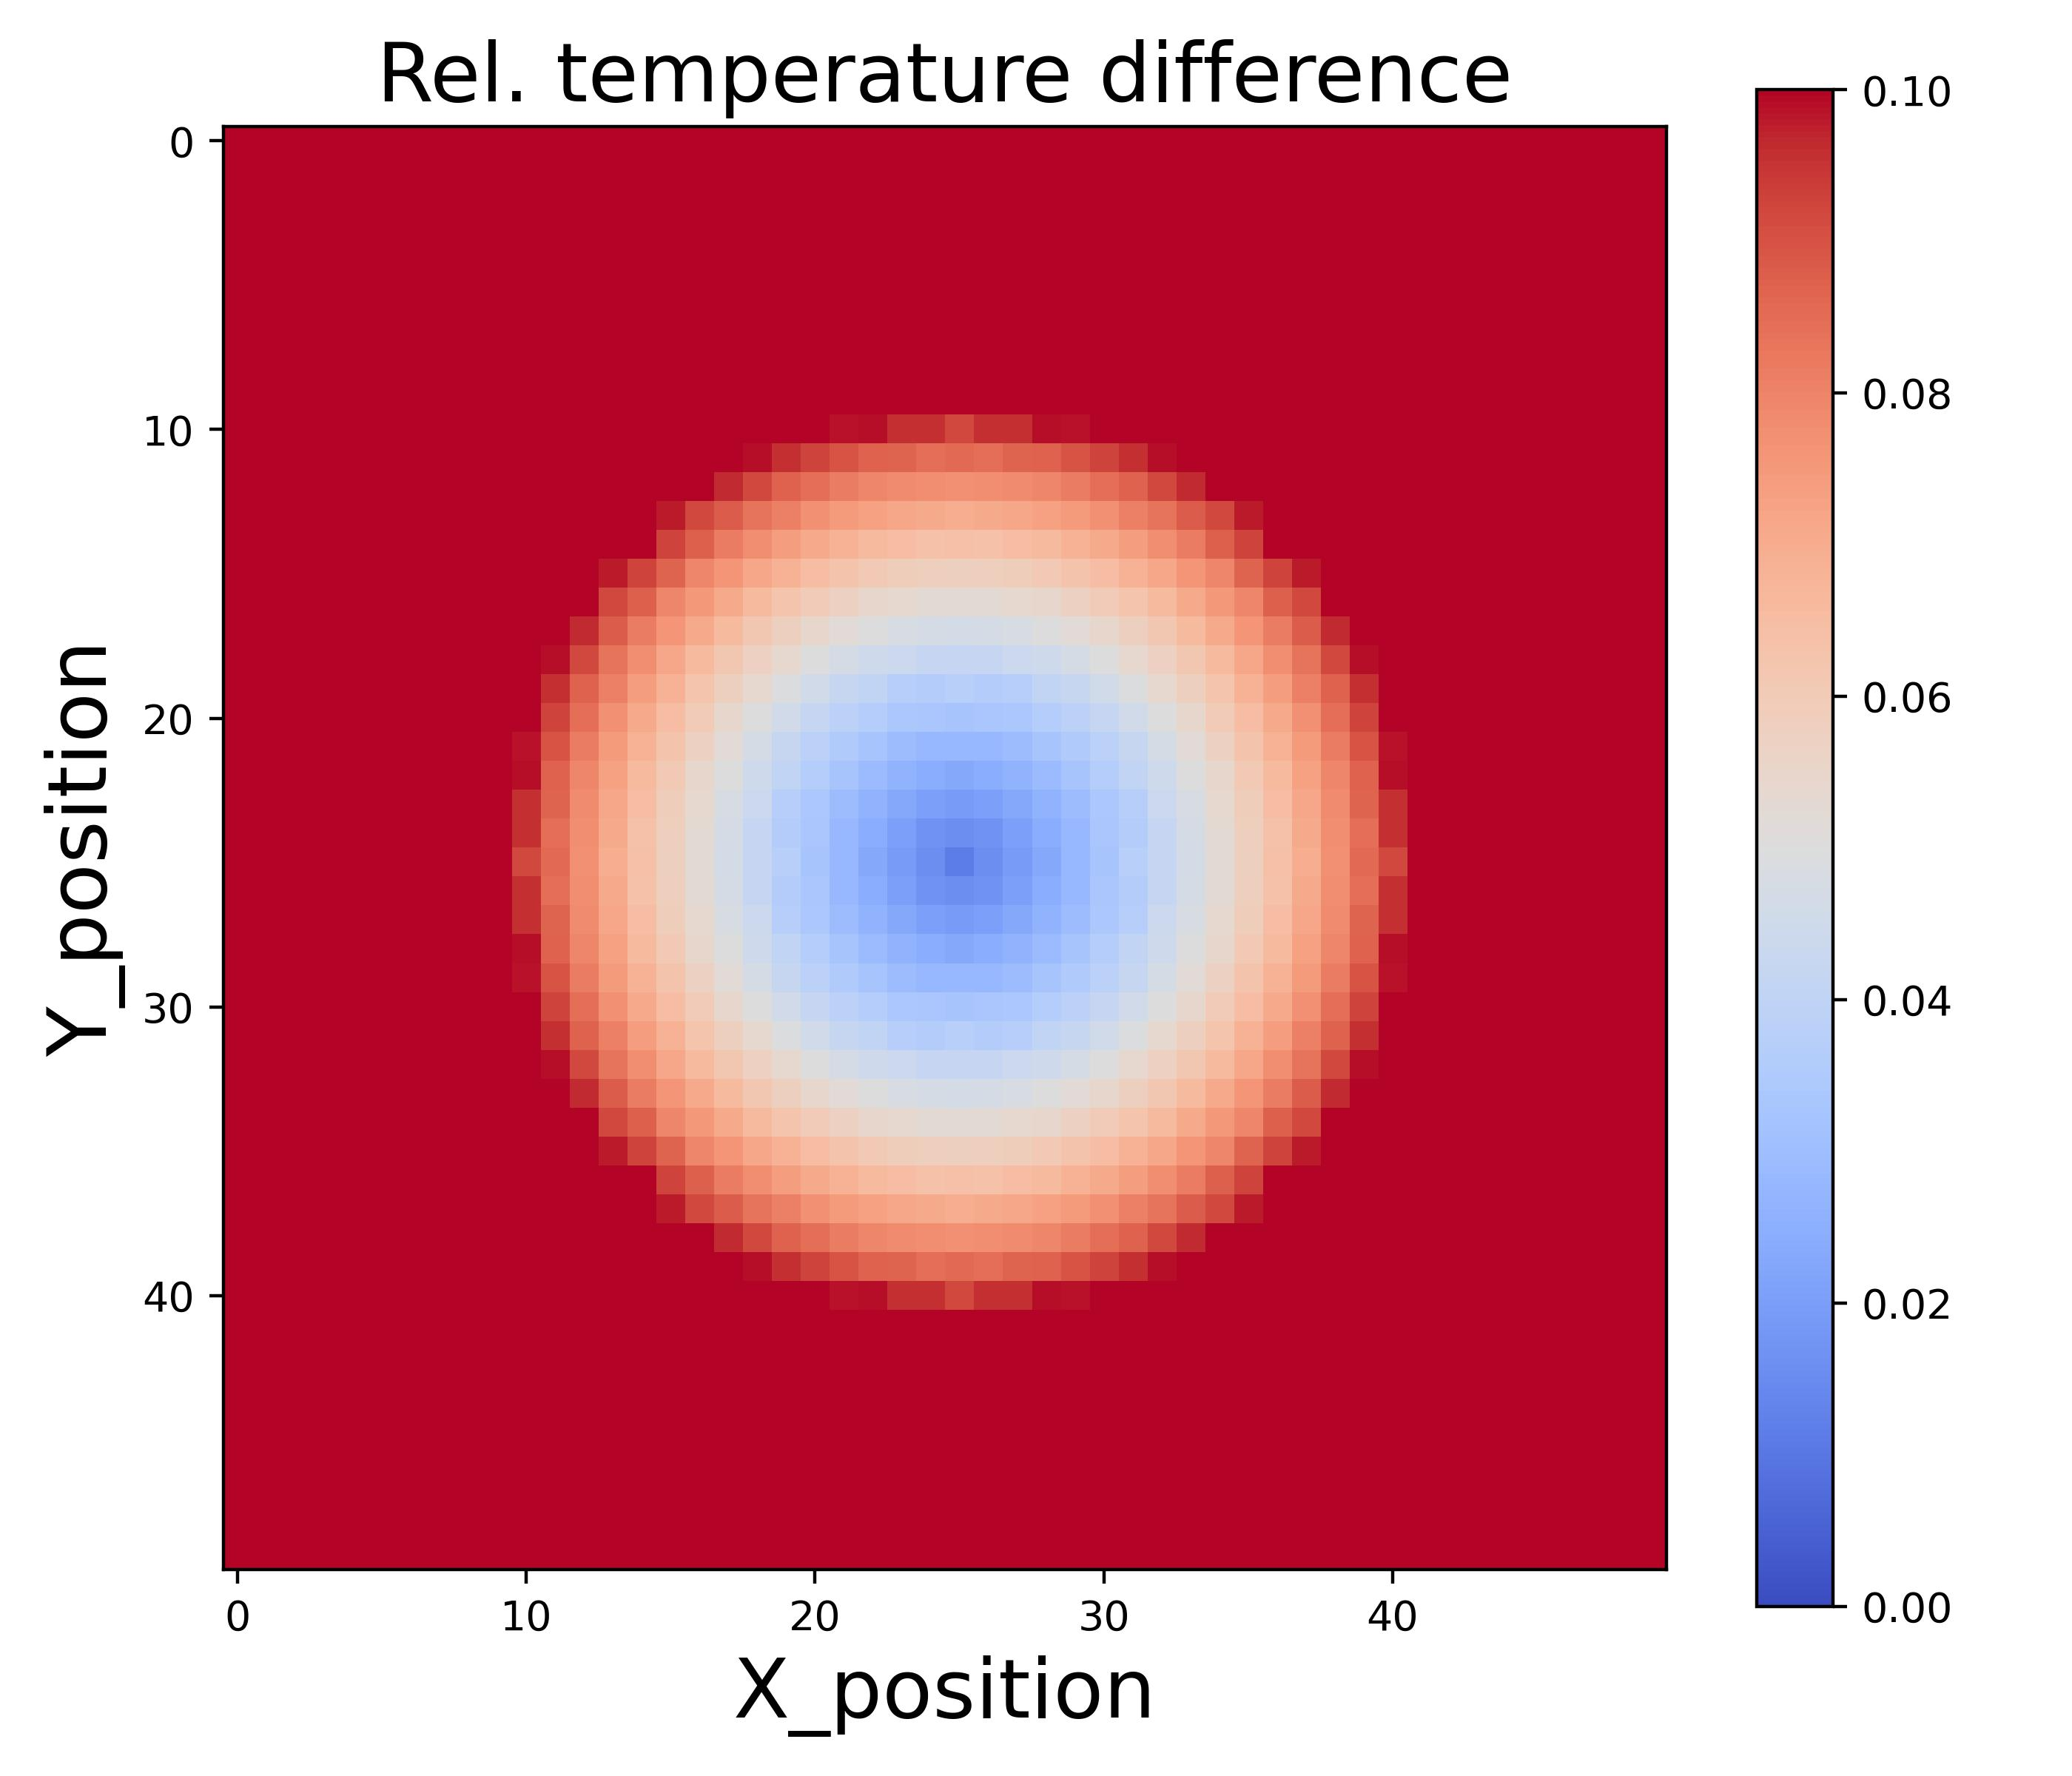
\includegraphics[width=\textwidth]{figures/raw_data/26/lin_square/T_bias.jpg}
            \subcaption{Model 6}
        \end{subfigure}
        \begin{subfigure}{0.325\textwidth}
            \centering
            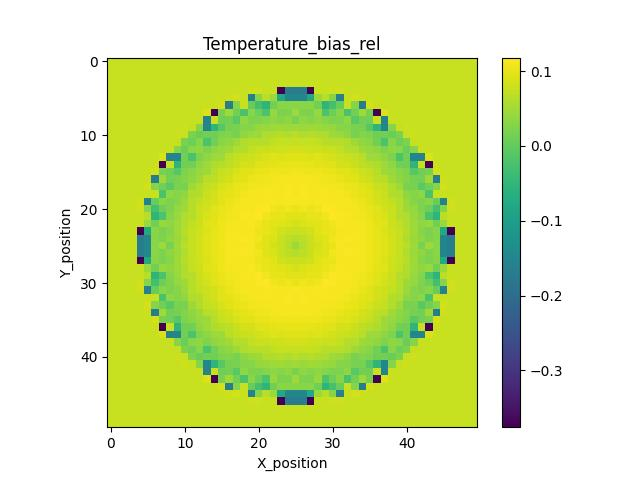
\includegraphics[width=\textwidth]{figures/raw_data/31/lin_square/T_bias.jpg}
            \subcaption{Model 7}
        \end{subfigure}
    \end{minipage}\\
    \begin{minipage}{\textwidth}
        \centering
        \begin{subfigure}{0.325\textwidth}
            \centering
            \includegraphics[width=\textwidth]{figures/raw_data/32/lin_square/T_bias.jpg}
            \subcaption{Model 8}
        \end{subfigure}
        \begin{subfigure}{0.325\textwidth}
            \centering
            \includegraphics[width=\textwidth]{figures/raw_data/33/lin_square/T_bias.jpg}
            \subcaption{Model 9}
        \end{subfigure}
    \end{minipage}
    \caption{Temperature calculation results of linear square model}  
\end{figure}
\begin{figure}[p]
    \centering
    \begin{minipage}{\textwidth}
        \centering
        \begin{subfigure}{0.325\textwidth}
            \centering
            \includegraphics[width=\textwidth]{figures/raw_data/0/lin_square/emi_cal.jpg}
            \subcaption{Black body material}
        \end{subfigure}
        \begin{subfigure}{0.325\textwidth}
            \centering
            \includegraphics[width=\textwidth]{figures/raw_data/5/lin_square/emi_cal.jpg}
            \subcaption{Real iron data}
        \end{subfigure}
        \begin{subfigure}{0.325\textwidth}
            \centering
            \includegraphics[width=\textwidth]{figures/raw_data/21/lin_square/emi_cal.jpg}
            \subcaption{Model 1}
        \end{subfigure}
    \end{minipage}\\
    \begin{minipage}{\textwidth}
        \centering
        \begin{subfigure}{0.325\textwidth}
            \centering
            \includegraphics[width=\textwidth]{figures/raw_data/22/lin_square/emi_cal.jpg}
            \subcaption{Model 2}
        \end{subfigure}
        \begin{subfigure}{0.325\textwidth}
            \centering
            \includegraphics[width=\textwidth]{figures/raw_data/23/lin_square/emi_cal.jpg}
            \subcaption{Model 3}
        \end{subfigure}
        \begin{subfigure}{0.325\textwidth}
            \centering
            \includegraphics[width=\textwidth]{figures/raw_data/24/lin_square/emi_cal.jpg}
            \subcaption{Model 4}
        \end{subfigure}
    \end{minipage}\\
    \begin{minipage}{\textwidth}
        \centering
        \begin{subfigure}{0.325\textwidth}
            \centering
            \includegraphics[width=\textwidth]{figures/raw_data/25/lin_square/emi_cal.jpg}
            \subcaption{Model 5}
        \end{subfigure}
        \begin{subfigure}{0.325\textwidth}
            \centering
            \includegraphics[width=\textwidth]{figures/raw_data/26/lin_square/emi_cal.jpg}
            \subcaption{Model 6}
        \end{subfigure}
        \begin{subfigure}{0.325\textwidth}
            \centering
            \includegraphics[width=\textwidth]{figures/raw_data/31/lin_square/emi_cal.jpg}
            \subcaption{Model 7}
        \end{subfigure}
    \end{minipage}\\
    \begin{minipage}{\textwidth}
        \centering
        \begin{subfigure}{0.325\textwidth}
            \centering
            \includegraphics[width=\textwidth]{figures/raw_data/32/lin_square/emi_cal.jpg}
            \subcaption{Model 8}
        \end{subfigure}
        \begin{subfigure}{0.325\textwidth}
            \centering
            \includegraphics[width=\textwidth]{figures/raw_data/33/lin_square/emi_cal.jpg}
            \subcaption{Model 9}
        \end{subfigure}
    \end{minipage}
    \caption{Emissivity calculation results of linear square model}  
\end{figure}


\newpage
\subsection{Quadratic model}
\begin{figure}[h]
    \centering
    \begin{minipage}{\textwidth}
        \centering
        \begin{subfigure}{0.325\textwidth}
            \centering
            \includegraphics[width=\textwidth]{figures/raw_data/0/quad/T_bias.jpg}
            \subcaption{Black body material}
        \end{subfigure}
        \begin{subfigure}{0.325\textwidth}
            \centering
            \includegraphics[width=\textwidth]{figures/raw_data/5/quad/T_bias.jpg}
            \subcaption{Real iron data}
        \end{subfigure}
        \begin{subfigure}{0.325\textwidth}
            \centering
            \includegraphics[width=\textwidth]{figures/raw_data/21/quad/T_bias.jpg}
            \subcaption{Model 1}
        \end{subfigure}
    \end{minipage}\\
    \begin{minipage}{\textwidth}
        \centering
        \begin{subfigure}{0.325\textwidth}
            \centering
            \includegraphics[width=\textwidth]{figures/raw_data/22/quad/T_bias.jpg}
            \subcaption{Model 2}
        \end{subfigure}
        \begin{subfigure}{0.325\textwidth}
            \centering
            \includegraphics[width=\textwidth]{figures/raw_data/23/quad/T_bias.jpg}
            \subcaption{Model 3}
        \end{subfigure}
        \begin{subfigure}{0.325\textwidth}
            \centering
            \includegraphics[width=\textwidth]{figures/raw_data/24/quad/T_bias.jpg}
            \subcaption{Model 4}
        \end{subfigure}
    \end{minipage}\\
    \begin{minipage}{\textwidth}
        \centering
        \begin{subfigure}{0.325\textwidth}
            \centering
            \includegraphics[width=\textwidth]{figures/raw_data/25/quad/T_bias.jpg}
            \subcaption{Model 5}
        \end{subfigure}
        \begin{subfigure}{0.325\textwidth}
            \centering
            \includegraphics[width=\textwidth]{figures/raw_data/26/quad/T_bias.jpg}
            \subcaption{Model 6}
        \end{subfigure}
        \begin{subfigure}{0.325\textwidth}
            \centering
            \includegraphics[width=\textwidth]{figures/raw_data/31/quad/T_bias.jpg}
            \subcaption{Model 7}
        \end{subfigure}
    \end{minipage}\\
    \begin{minipage}{\textwidth}
        \centering
        \begin{subfigure}{0.325\textwidth}
            \centering
            \includegraphics[width=\textwidth]{figures/raw_data/32/quad/T_bias.jpg}
            \subcaption{Model 8}
        \end{subfigure}
        \begin{subfigure}{0.325\textwidth}
            \centering
            \includegraphics[width=\textwidth]{figures/raw_data/33/quad/T_bias.jpg}
            \subcaption{Model 9}
        \end{subfigure}
    \end{minipage}
    \caption{Temperature calculation results of quadratic model}  
\end{figure}
\begin{figure}[p]
    \centering
    \begin{minipage}{\textwidth}
        \centering
        \begin{subfigure}{0.325\textwidth}
            \centering
            \includegraphics[width=\textwidth]{figures/raw_data/0/quad/emi_cal.jpg}
            \subcaption{Black body material}
        \end{subfigure}
        \begin{subfigure}{0.325\textwidth}
            \centering
            \includegraphics[width=\textwidth]{figures/raw_data/5/quad/emi_cal.jpg}
            \subcaption{Real iron data}
        \end{subfigure}
        \begin{subfigure}{0.325\textwidth}
            \centering
            \includegraphics[width=\textwidth]{figures/raw_data/21/quad/emi_cal.jpg}
            \subcaption{Model 1}
        \end{subfigure}
    \end{minipage}\\
    \begin{minipage}{\textwidth}
        \centering
        \begin{subfigure}{0.325\textwidth}
            \centering
            \includegraphics[width=\textwidth]{figures/raw_data/22/quad/emi_cal.jpg}
            \subcaption{Model 2}
        \end{subfigure}
        \begin{subfigure}{0.325\textwidth}
            \centering
            \includegraphics[width=\textwidth]{figures/raw_data/23/quad/emi_cal.jpg}
            \subcaption{Model 3}
        \end{subfigure}
        \begin{subfigure}{0.325\textwidth}
            \centering
            \includegraphics[width=\textwidth]{figures/raw_data/24/quad/emi_cal.jpg}
            \subcaption{Model 4}
        \end{subfigure}
    \end{minipage}\\
    \begin{minipage}{\textwidth}
        \centering
        \begin{subfigure}{0.325\textwidth}
            \centering
            \includegraphics[width=\textwidth]{figures/raw_data/25/quad/emi_cal.jpg}
            \subcaption{Model 5}
        \end{subfigure}
        \begin{subfigure}{0.325\textwidth}
            \centering
            \includegraphics[width=\textwidth]{figures/raw_data/26/quad/emi_cal.jpg}
            \subcaption{Model 6}
        \end{subfigure}
        \begin{subfigure}{0.325\textwidth}
            \centering
            \includegraphics[width=\textwidth]{figures/raw_data/31/quad/emi_cal.jpg}
            \subcaption{Model 7}
        \end{subfigure}
    \end{minipage}\\
    \begin{minipage}{\textwidth}
        \centering
        \begin{subfigure}{0.325\textwidth}
            \centering
            \includegraphics[width=\textwidth]{figures/raw_data/32/quad/emi_cal.jpg}
            \subcaption{Model 8}
        \end{subfigure}
        \begin{subfigure}{0.325\textwidth}
            \centering
            \includegraphics[width=\textwidth]{figures/raw_data/33/quad/emi_cal.jpg}
            \subcaption{Model 9}
        \end{subfigure}
    \end{minipage}
    \caption{Emissivity calculation results of quadratic model}  
\end{figure}


\newpage
\subsection{Exponential model}
\begin{figure}[h]
    \centering
    \begin{minipage}{\textwidth}
        \centering
        \begin{subfigure}{0.325\textwidth}
            \centering
            \includegraphics[width=\textwidth]{figures/raw_data/0/exp/T_bias.jpg}
            \subcaption{Black body material}
        \end{subfigure}
        \begin{subfigure}{0.325\textwidth}
            \centering
            \includegraphics[width=\textwidth]{figures/raw_data/5/exp/T_bias.jpg}
            \subcaption{Real iron data}
        \end{subfigure}
        \begin{subfigure}{0.325\textwidth}
            \centering
            \includegraphics[width=\textwidth]{figures/raw_data/21/exp/T_bias.jpg}
            \subcaption{Model 1}
        \end{subfigure}
    \end{minipage}\\
    \begin{minipage}{\textwidth}
        \centering
        \begin{subfigure}{0.325\textwidth}
            \centering
            \includegraphics[width=\textwidth]{figures/raw_data/22/exp/T_bias.jpg}
            \subcaption{Model 2}
        \end{subfigure}
        \begin{subfigure}{0.325\textwidth}
            \centering
            \includegraphics[width=\textwidth]{figures/raw_data/23/exp/T_bias.jpg}
            \subcaption{Model 3}
        \end{subfigure}
        \begin{subfigure}{0.325\textwidth}
            \centering
            \includegraphics[width=\textwidth]{figures/raw_data/24/exp/T_bias.jpg}
            \subcaption{Model 4}
        \end{subfigure}
    \end{minipage}\\
    \begin{minipage}{\textwidth}
        \centering
        \begin{subfigure}{0.325\textwidth}
            \centering
            \includegraphics[width=\textwidth]{figures/raw_data/25/exp/T_bias.jpg}
            \subcaption{Model 5}
        \end{subfigure}
        \begin{subfigure}{0.325\textwidth}
            \centering
            \includegraphics[width=\textwidth]{figures/raw_data/26/exp/T_bias.jpg}
            \subcaption{Model 6}
        \end{subfigure}
        \begin{subfigure}{0.325\textwidth}
            \centering
            \includegraphics[width=\textwidth]{figures/raw_data/31/exp/T_bias.jpg}
            \subcaption{Model 7}
        \end{subfigure}
    \end{minipage}\\
    \begin{minipage}{\textwidth}
        \centering
        \begin{subfigure}{0.325\textwidth}
            \centering
            \includegraphics[width=\textwidth]{figures/raw_data/32/exp/T_bias.jpg}
            \subcaption{Model 8}
        \end{subfigure}
        \begin{subfigure}{0.325\textwidth}
            \centering
            \includegraphics[width=\textwidth]{figures/raw_data/33/exp/T_bias.jpg}
            \subcaption{Model 9}
        \end{subfigure}
    \end{minipage}
    \caption{Temperature calculation results of exponential model}  
\end{figure}
\begin{figure}[p]
    \centering
    \begin{minipage}{\textwidth}
        \centering
        \begin{subfigure}{0.325\textwidth}
            \centering
            \includegraphics[width=\textwidth]{figures/raw_data/0/exp/emi_cal.jpg}
            \subcaption{Black body material}
        \end{subfigure}
        \begin{subfigure}{0.325\textwidth}
            \centering
            \includegraphics[width=\textwidth]{figures/raw_data/5/exp/emi_cal.jpg}
            \subcaption{Real iron data}
        \end{subfigure}
        \begin{subfigure}{0.325\textwidth}
            \centering
            \includegraphics[width=\textwidth]{figures/raw_data/21/exp/emi_cal.jpg}
            \subcaption{Model 1}
        \end{subfigure}
    \end{minipage}\\
    \begin{minipage}{\textwidth}
        \centering
        \begin{subfigure}{0.325\textwidth}
            \centering
            \includegraphics[width=\textwidth]{figures/raw_data/22/exp/emi_cal.jpg}
            \subcaption{Model 2}
        \end{subfigure}
        \begin{subfigure}{0.325\textwidth}
            \centering
            \includegraphics[width=\textwidth]{figures/raw_data/23/exp/emi_cal.jpg}
            \subcaption{Model 3}
        \end{subfigure}
        \begin{subfigure}{0.325\textwidth}
            \centering
            \includegraphics[width=\textwidth]{figures/raw_data/24/exp/emi_cal.jpg}
            \subcaption{Model 4}
        \end{subfigure}
    \end{minipage}\\
    \begin{minipage}{\textwidth}
        \centering
        \begin{subfigure}{0.325\textwidth}
            \centering
            \includegraphics[width=\textwidth]{figures/raw_data/25/exp/emi_cal.jpg}
            \subcaption{Model 5}
        \end{subfigure}
        \begin{subfigure}{0.325\textwidth}
            \centering
            \includegraphics[width=\textwidth]{figures/raw_data/26/exp/emi_cal.jpg}
            \subcaption{Model 6}
        \end{subfigure}
        \begin{subfigure}{0.325\textwidth}
            \centering
            \includegraphics[width=\textwidth]{figures/raw_data/31/exp/emi_cal.jpg}
            \subcaption{Model 7}
        \end{subfigure}
    \end{minipage}\\
    \begin{minipage}{\textwidth}
        \centering
        \begin{subfigure}{0.325\textwidth}
            \centering
            \includegraphics[width=\textwidth]{figures/raw_data/32/exp/emi_cal.jpg}
            \subcaption{Model 8}
        \end{subfigure}
        \begin{subfigure}{0.325\textwidth}
            \centering
            \includegraphics[width=\textwidth]{figures/raw_data/33/exp/emi_cal.jpg}
            \subcaption{Model 9}
        \end{subfigure}
    \end{minipage}
    \caption{Emissivity calculation results of exponential model}  
\end{figure}


\newpage
\subsection{Mixed model}
\begin{figure}[h]
    \centering
    \begin{minipage}{\textwidth}
        \centering
        \begin{subfigure}{0.325\textwidth}
            \centering
            \includegraphics[width=\textwidth]{figures/raw_data/0/mix/T_bias.jpg}
            \subcaption{Black body material}
        \end{subfigure}
        \begin{subfigure}{0.325\textwidth}
            \centering
            \includegraphics[width=\textwidth]{figures/raw_data/5/mix/T_bias.jpg}
            \subcaption{Real iron data}
        \end{subfigure}
        \begin{subfigure}{0.325\textwidth}
            \centering
            \includegraphics[width=\textwidth]{figures/raw_data/21/mix/T_bias.jpg}
            \subcaption{Model 1}
        \end{subfigure}
    \end{minipage}\\
    \begin{minipage}{\textwidth}
        \centering
        \begin{subfigure}{0.325\textwidth}
            \centering
            \includegraphics[width=\textwidth]{figures/raw_data/22/mix/T_bias.jpg}
            \subcaption{Model 2}
        \end{subfigure}
        \begin{subfigure}{0.325\textwidth}
            \centering
            \includegraphics[width=\textwidth]{figures/raw_data/23/mix/T_bias.jpg}
            \subcaption{Model 3}
        \end{subfigure}
        \begin{subfigure}{0.325\textwidth}
            \centering
            \includegraphics[width=\textwidth]{figures/raw_data/24/mix/T_bias.jpg}
            \subcaption{Model 4}
        \end{subfigure}
    \end{minipage}\\
    \begin{minipage}{\textwidth}
        \centering
        \begin{subfigure}{0.325\textwidth}
            \centering
            \includegraphics[width=\textwidth]{figures/raw_data/25/mix/T_bias.jpg}
            \subcaption{Model 5}
        \end{subfigure}
        \begin{subfigure}{0.325\textwidth}
            \centering
            \includegraphics[width=\textwidth]{figures/raw_data/26/mix/T_bias.jpg}
            \subcaption{Model 6}
        \end{subfigure}
        \begin{subfigure}{0.325\textwidth}
            \centering
            \includegraphics[width=\textwidth]{figures/raw_data/31/mix/T_bias.jpg}
            \subcaption{Model 7}
        \end{subfigure}
    \end{minipage}\\
    \begin{minipage}{\textwidth}
        \centering
        \begin{subfigure}{0.325\textwidth}
            \centering
            \includegraphics[width=\textwidth]{figures/raw_data/32/mix/T_bias.jpg}
            \subcaption{Model 8}
        \end{subfigure}
        \begin{subfigure}{0.325\textwidth}
            \centering
            \includegraphics[width=\textwidth]{figures/raw_data/33/mix/T_bias.jpg}
            \subcaption{Model 9}
        \end{subfigure}
    \end{minipage}
    \caption{Temperature calculation results of mixed model}  
\end{figure}
\begin{figure}[p]
    \centering
    \begin{minipage}{\textwidth}
        \centering
        \begin{subfigure}{0.325\textwidth}
            \centering
            \includegraphics[width=\textwidth]{figures/raw_data/0/mix/emi_cal.jpg}
            \subcaption{Black body material}
        \end{subfigure}
        \begin{subfigure}{0.325\textwidth}
            \centering
            \includegraphics[width=\textwidth]{figures/raw_data/5/mix/emi_cal.jpg}
            \subcaption{Real iron data}
        \end{subfigure}
        \begin{subfigure}{0.325\textwidth}
            \centering
            \includegraphics[width=\textwidth]{figures/raw_data/21/mix/emi_cal.jpg}
            \subcaption{Model 1}
        \end{subfigure}
    \end{minipage}\\
    \begin{minipage}{\textwidth}
        \centering
        \begin{subfigure}{0.325\textwidth}
            \centering
            \includegraphics[width=\textwidth]{figures/raw_data/22/mix/emi_cal.jpg}
            \subcaption{Model 2}
        \end{subfigure}
        \begin{subfigure}{0.325\textwidth}
            \centering
            \includegraphics[width=\textwidth]{figures/raw_data/23/mix/emi_cal.jpg}
            \subcaption{Model 3}
        \end{subfigure}
        \begin{subfigure}{0.325\textwidth}
            \centering
            \includegraphics[width=\textwidth]{figures/raw_data/24/mix/emi_cal.jpg}
            \subcaption{Model 4}
        \end{subfigure}
    \end{minipage}\\
    \begin{minipage}{\textwidth}
        \centering
        \begin{subfigure}{0.325\textwidth}
            \centering
            \includegraphics[width=\textwidth]{figures/raw_data/25/mix/emi_cal.jpg}
            \subcaption{Model 5}
        \end{subfigure}
        \begin{subfigure}{0.325\textwidth}
            \centering
            \includegraphics[width=\textwidth]{figures/raw_data/26/mix/emi_cal.jpg}
            \subcaption{Model 6}
        \end{subfigure}
        \begin{subfigure}{0.325\textwidth}
            \centering
            \includegraphics[width=\textwidth]{figures/raw_data/31/mix/emi_cal.jpg}
            \subcaption{Model 7}
        \end{subfigure}
    \end{minipage}\\
    \begin{minipage}{\textwidth}
        \centering
        \begin{subfigure}{0.325\textwidth}
            \centering
            \includegraphics[width=\textwidth]{figures/raw_data/32/mix/emi_cal.jpg}
            \subcaption{Model 8}
        \end{subfigure}
        \begin{subfigure}{0.325\textwidth}
            \centering
            \includegraphics[width=\textwidth]{figures/raw_data/33/mix/emi_cal.jpg}
            \subcaption{Model 9}
        \end{subfigure}
    \end{minipage}
    \caption{Emissivity calculation results of mixed model}  
\end{figure}%
%
% Glossary
% ---------------------
\printnoidxglossary[sort=standard,title={\IWBlangGlossary}]
%
% References
% ----------
\printbibliography[heading=bibintoc, title={\IWBlangBibliography}]%
%
%
% List of Abbreviations
% ---------------------
\printnoidxglossary[type=acronym,sort=standard,title={\IWBlangAcronyms}]
%
%
\end{document}%
%
%
